\chapter{Calorimeter Optimisation Studies}
\label{chap:detopt}

\chapterquote{The simple believes everything, but the prudent gives thought to his steps.}
{Proverbs 14:15}

%========================================================================================
%========================================================================================

\section{Introduction}
\label{sec:optimisationstudies}
This chapter describes the optimisation of the calorimeters used at the linear collider, with focus placed on obtaining the best energy resolution for jets.  Parameters such as the number of layers, cell size and material choices for the calorimeters are investigated.  Several global detector parameters such as the magnetic field strength and the inner radius of the ECal are also studied.  These parameters are not calorimeter specific, but affect the jet energy resolution obtained from particle flow. 

%========================================================================================
%========================================================================================

\section{Electromagnetic Calorimeter Optimisation}
\label{sec:ecal}
The purpose of an electromagnetic calorimeter (ECal) is to measure the energy deposits from electromagnetic showers.  The nominal ILD ECal, summarised in table \ref{table:defaultildecal}, is a silicon-tungsten sampling calorimeter.  It contains 29 readout layers and 24 radiation lengths ($\text{X}_{0}$), which is sufficient to contain all but the highest energy electromagnetic showers.  The absorber thickness of the last nine layers is twice that of the first 20 layers to reduce the number of readout channels and cost of the calorimeter.  The high longitudinal sampling frequency is crucial for the pattern recognition aspect of particle flow calorimetry, especially in the region where particle showers start developing.  

\begin{table}[h!]
\centering
\begin{tabular}{ l l}
\hline
Parameter & Default Value \\
\hline
Cell Size & $5 \times 5\text{ mm}^{2}$ square cells \\
Number of Layers & 29 readout layers \\
Active Material Choice & Silicon or Scintillator  \\
Active Material Thickness & 0.5 mm (Silicon) or 2 mm (Scintillator)  \\
Absorber Material Choice & Tungsten \\
Absorber Material Thickness & 20 layers of 2.1 mm followed by 9 layers of 4.2 mm \\
\hline
\end{tabular}
\caption[The configuration of the silicon and scintillator ECal options for the ILD detector model \cite{Behnke:2013lya}.]{The configuration of the silicon and scintillator ECal options for the ILD detector model \cite{Behnke:2013lya}.}
\label{table:defaultildecal}
\end{table}

The calorimeter performance was simulated for a number of detector models where the following detector parameters were varied:
\begin{itemize}
\item Cell size:  This is a vital aspect of the detector in the particle flow paradigm as smaller cell sizes leads to better separation between nearby showering particles, which helps to minimise the effect of confusion.  Modifying the cell size should have little effect on the intrinsic energy resolution of the detector.  
\item Longitudinal sampling frequency:  The longitudinal sampling frequency in the ECal was varied by changing the number of layers in the ECal while simultaneously changing the thicknesses of the layers such that the total depth, in radiation lengths, was held constant.  Increasing the number of layers in a sampling calorimeter means any particles showering within it are sampled more, which leads to a reduction in the stochastic contribution to the energy resolution.  Therefore, varying the number of layers is expected to change in intrinsic energy resolution of the calorimeter.  
\item Active material choice:  The options under consideration for the active sensor material are silicon or plastic scintillator.  As well as providing different intrinsic energy resolutions the readout mechanics of these two options are significantly different.  There is no clear prior knowledge as to which should provide better performance. 
\end{itemize}

%========================================================================================

\subsection{ECal Cell Size}
\label{sec:ecalcells}
Different detector models were considered where the cell size in the ECal was varied about the nominal value of $5 \times 5 \text{ mm}^{2}$ square cells.  The granularities considered were $3 \times 3 \text{ mm}^{2}$, $5 \times 5 \text{ mm}^{2}$, $7 \times 7 \text{ mm}^{2}$, $10 \times 10 \text{ mm}^{2}$, $15 \times 15 \text{ mm}^{2}$ and $20 \times 20 \text{ mm}^{2}$ square cells for both the silicon and scintillator active material options.  

The energy resolution, using 100~GeV photons, as a function of the ECal cell size is shown in figure \ref{fig:ecalsicellsize100gamma} for the silicon option and in figure \ref{fig:ecalsccellsize100gamma} for the scintillator option.  At this energy, the photons will be largely contained within the ECal and the reported energy resolution reflects solely the performance of the ECal.  For both the silicon and scintillator ECal options the energy resolution does not depend strongly on the ECal cell size.  This is to be expected as there is no change in the number of layers, which is the main factor in determining the energy resolution of a sampling calorimeter.  

The only statistically significant variation observed occurs for the scintillator ECal option.  A degradation in the energy resolution of $\sim10$\% is observed when reducing the ECal cell size from $5 \times 5 \text{ mm}^{2}$ to $3 \times 3 \text{ mm}^{2}$.  The most likely cause is the "dead" region in the active material, which represents the readout multi pixel photon counter (MPPC) \cite{arXiv:1006.3396}.  The MPPC occupies a fixed area of the cell, irrespective of cell size, and so the dead region of the cell fractionally increases as cell size is reduced.  The larger this dead region, the worse the sampling of the electromagnetic showers in the ECal and the worse the resolution.  While this effect will be present in all scintillator ECal options, it will only be significant for the small cell sizes when the dead region is fractionally the largest.    

\begin{figure}[h!]
\centering
\subfloat[]{\label{fig:ecalsicellsize100gamma}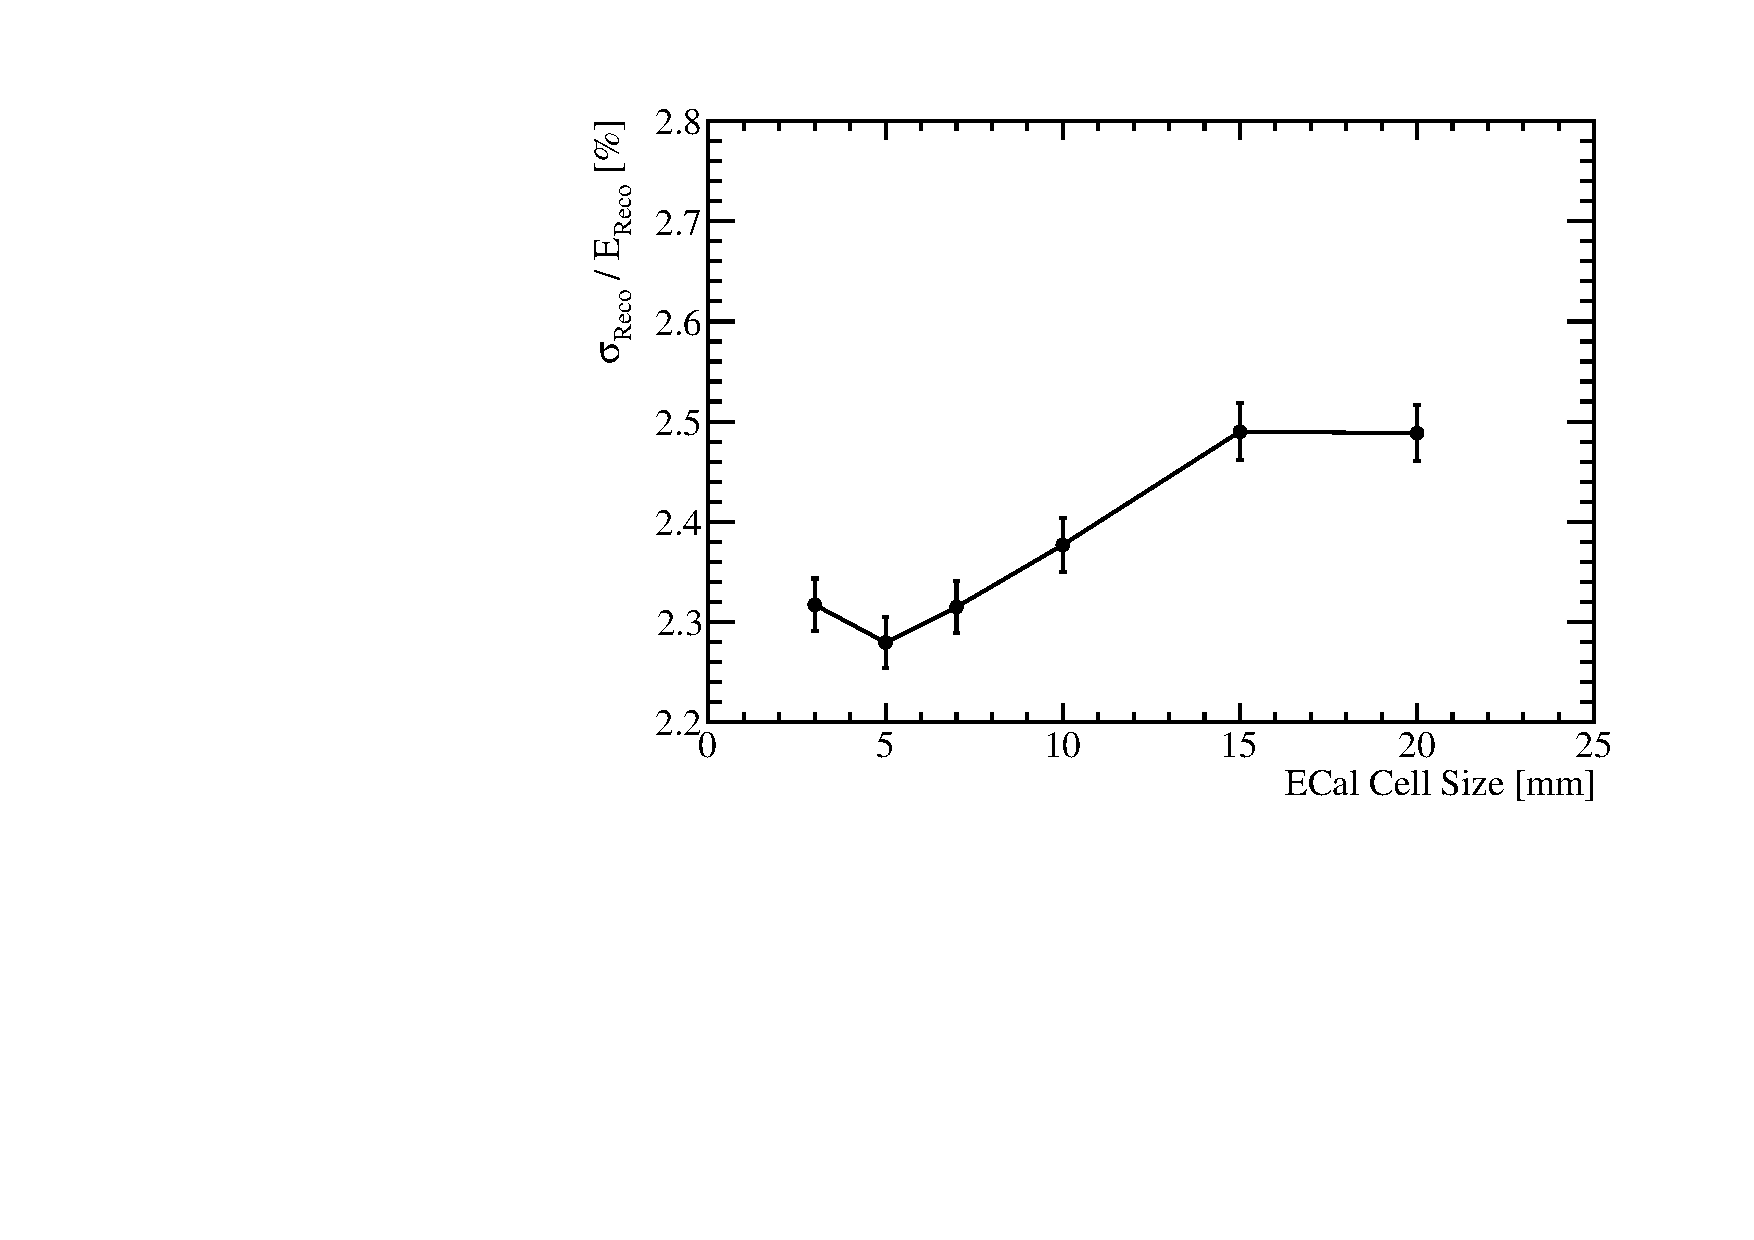
\includegraphics[width=0.5\textwidth]{OptimisationStudies/Plots/EnergyResolution/ER_vs_SiECalCellSize_100GeVPhoton.pdf}}
\subfloat[]{\label{fig:ecalsccellsize100gamma}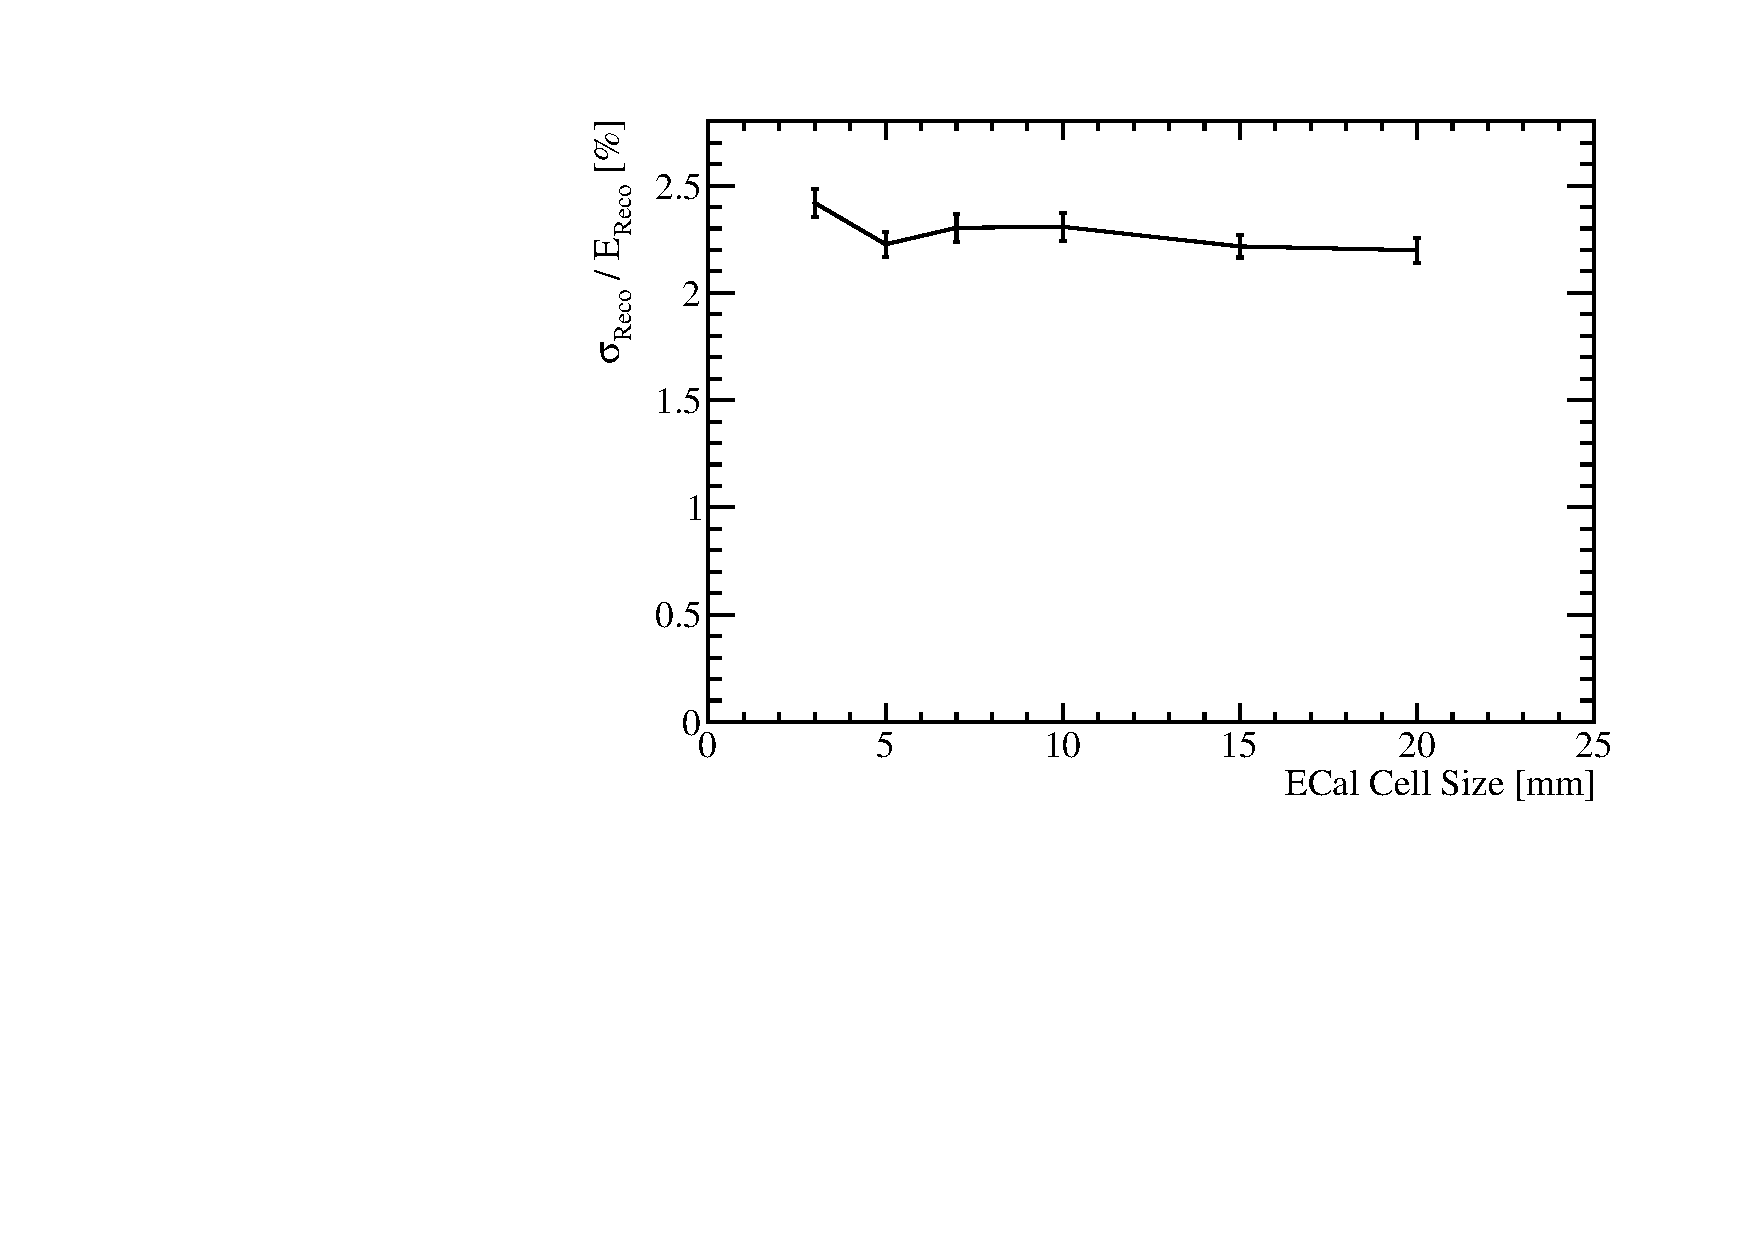
\includegraphics[width=0.5\textwidth]{OptimisationStudies/Plots/EnergyResolution/ER_vs_ScECalCellSize_100GeVPhoton.pdf}}
\caption[The energy resolution as a function of ECal cell size for 100~GeV photons using the nominal ILD detector model with \protect\subref{fig:ecalsicellsize100gamma} the silicon and \protect\subref{fig:ecalsccellsize100gamma} the scintillator ECal option.]{The energy resolution as a function of ECal cell size for 100~GeV photons using the nominal ILD detector model with \protect\subref{fig:ecalsicellsize100gamma} the silicon and \protect\subref{fig:ecalsccellsize100gamma} the scintillator ECal option.}
\label{fig:ecalcellsizegamma}
\end{figure}

The ability to separate nearby electromagnetic particle showers within a calorimeter is limited by the Moli�re radius of the absorber material and the cell size.  The Moli�re radius controls the width of the electromagnetic shower, while the cell size controls how the transverse shower profile is sampled.  By reducing the cell size, it becomes easier to resolve nearby electromagnetic showers, which in turn reduces the effect of confusion.  Therefore, it is expected that the jet energy resolution will be sensitive to the ECal cell size, even though the intrinsic energy resolution is not.  The jet energy resolution as a function of ECal cell size is shown in figure \ref{fig:ecalsicellsize} for the silicon option and figure \ref{fig:ecalsccellsize} for the scintillator option.  There is a strong dependance on the ECal cell size, with smaller cell sizes leading to lower values of the jet energy resolution; the jet energy resolution for 250~GeV jets for both ECal options goes from $\sim 3.0\%$ to $\sim 4.3\%$ when the ECal cell size goes from $3 \times 3 \text{ mm}^{2}$ to $20 \times 20 \text{ mm}^{2}$.  The origin of this trend is best illustrated by considering the intrinsic energy resolution and confusion contributions to the jet energy resolution.  These contributions are shown as a function of ECal cell size for 45 and 250~GeV jets in figure \ref{fig:ecalcellsizebreak}.  It is clear from these contributions that the intrinsic energy resolution of the detector does not change when varying the cell size, which agrees with both prior expectations of calorimeter behaviour and the single particle energy resolution study.  As expected, it can be seen that the trend in jet energy resolution as a function of the ECal cell size is being driven purely by changes to the confusion contribution and, in particular, the confusion caused by the reconstruction of photons.  

\begin{figure}[h!]
\centering
\subfloat[]{\label{fig:ecalsicellsize}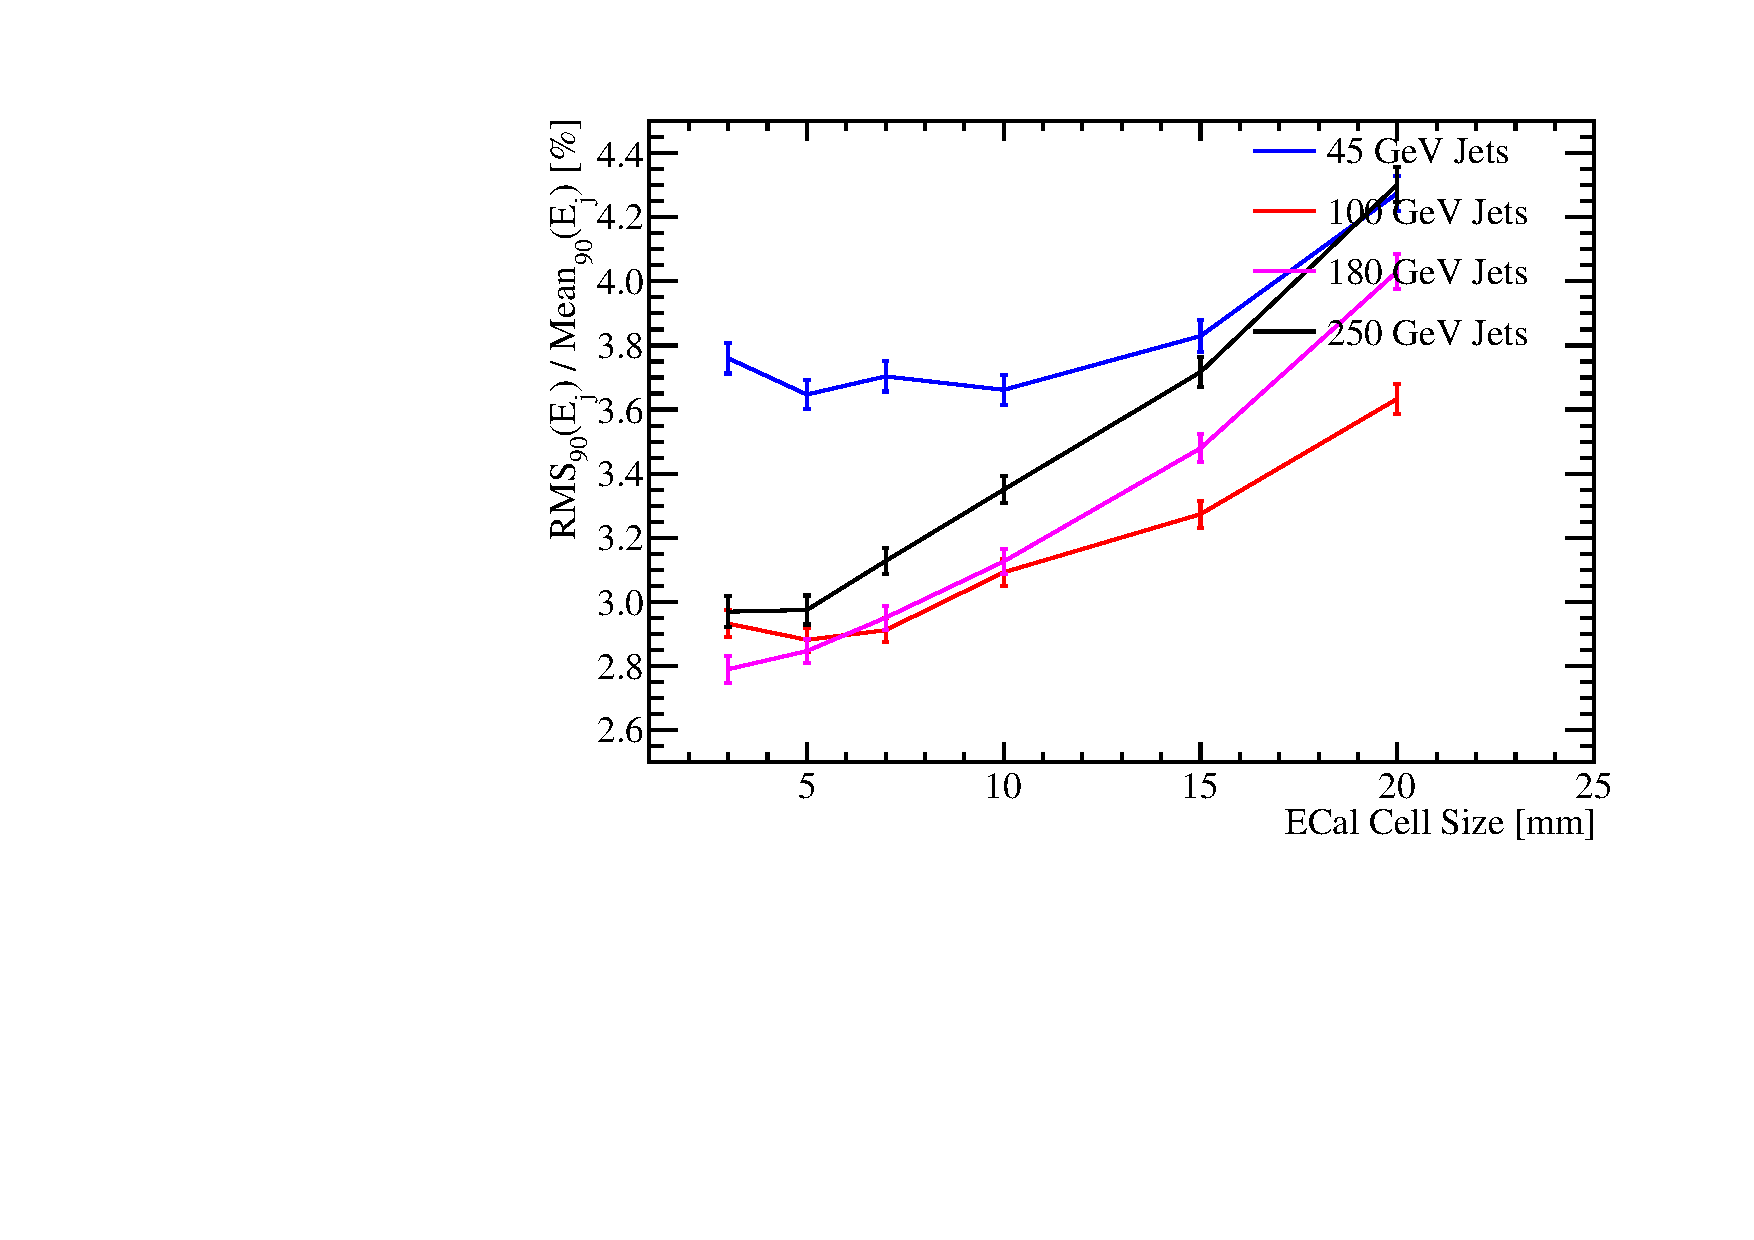
\includegraphics[width=0.5\textwidth]{OptimisationStudies/Plots/JetEnergyResolutions/JER_vs_SiliconECalCellSize.pdf}}
\subfloat[]{\label{fig:ecalsccellsize}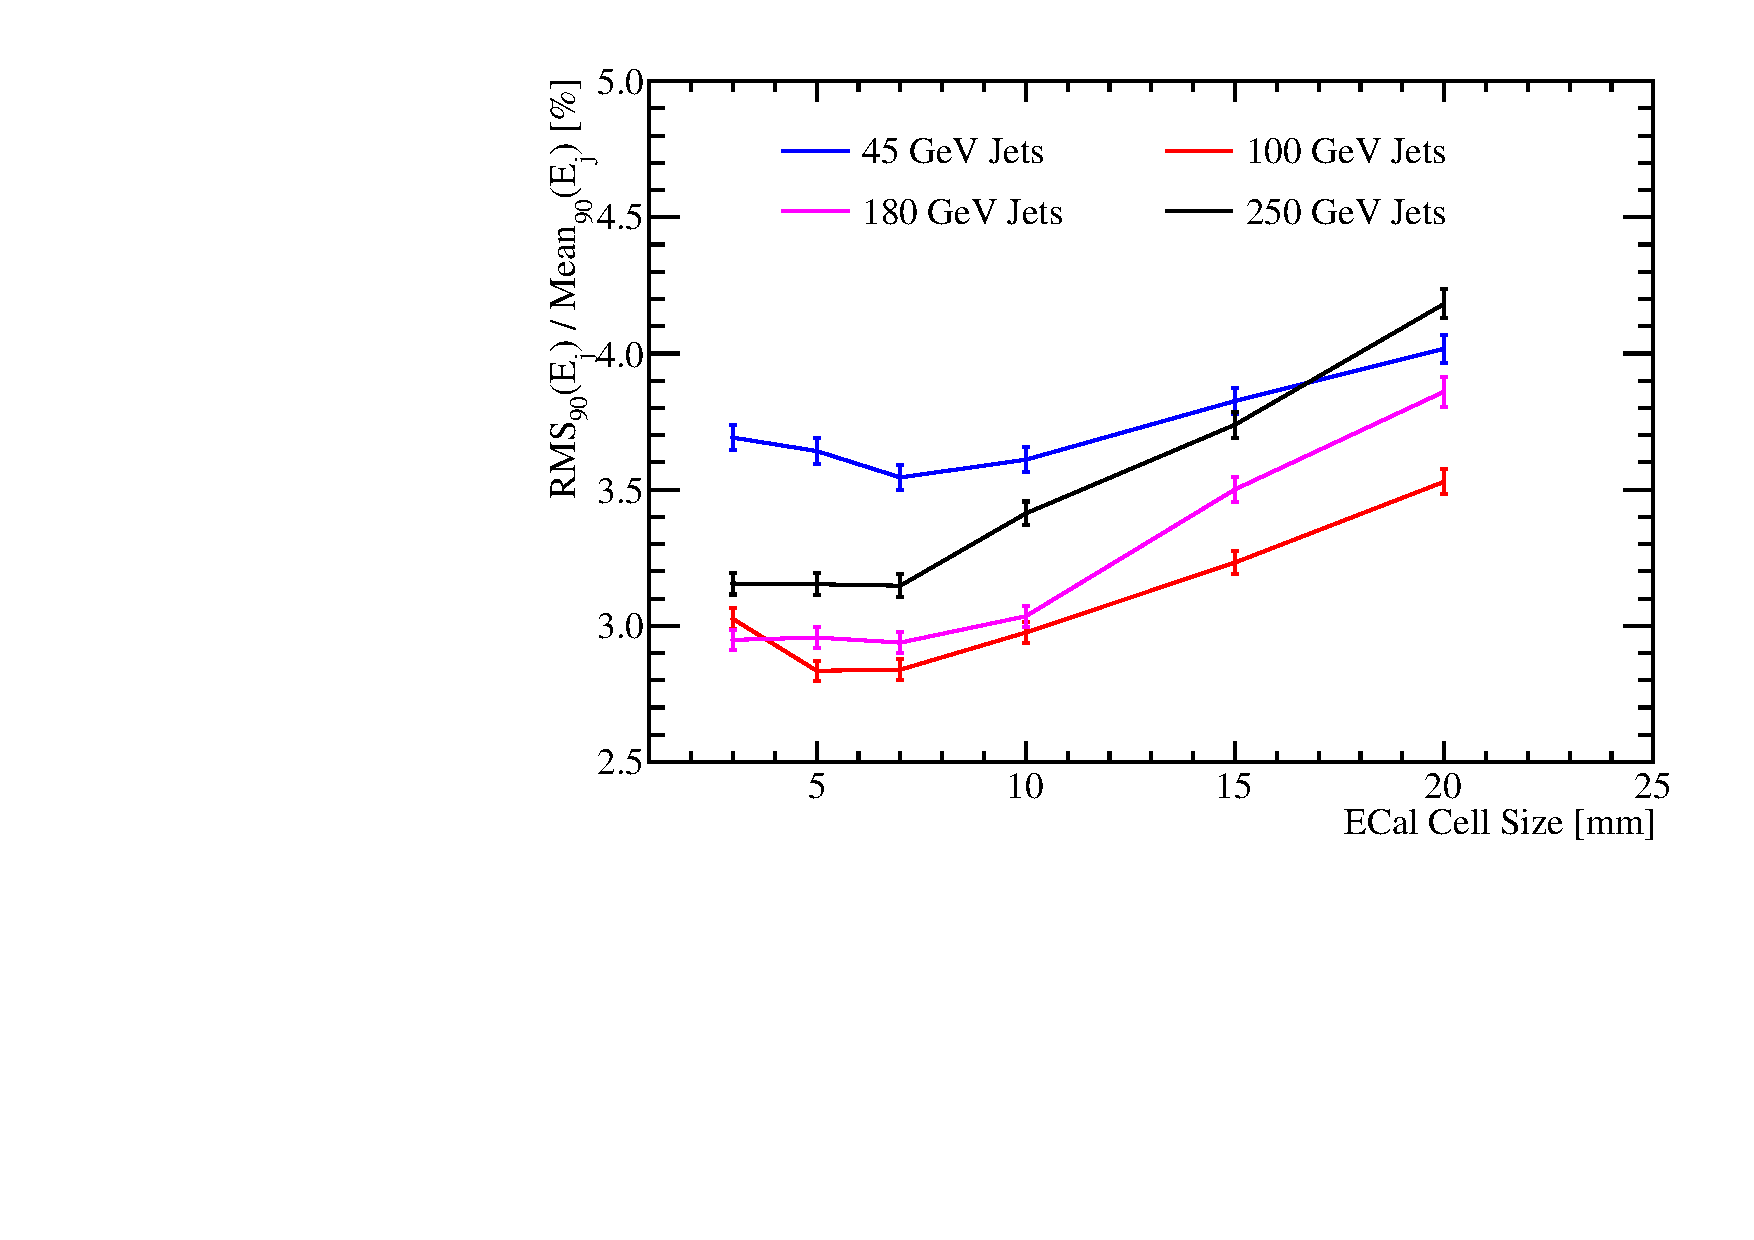
\includegraphics[width=0.5\textwidth]{OptimisationStudies/Plots/JetEnergyResolutions/JER_vs_ScintillatorECalCellSize.pdf}} \hfill
\caption[The fractional jet energy resolution as a function of ECal cell size for various jet energies using the nominal ILD detector model with \protect\subref{fig:ecalsicellsize} the silicon and \protect\subref{fig:ecalsccellsize} the scintillator ECal option.]{The fractional jet energy resolution as a function of ECal cell size for various jet energies using the nominal ILD detector model with \protect\subref{fig:ecalsicellsize} the silicon and \protect\subref{fig:ecalsccellsize} the scintillator ECal option.}
\label{fig:ecalcellsize}
\end{figure}

\begin{figure}[h!]
\centering
\subfloat[]{\label{fig:ecalsicellsize45break}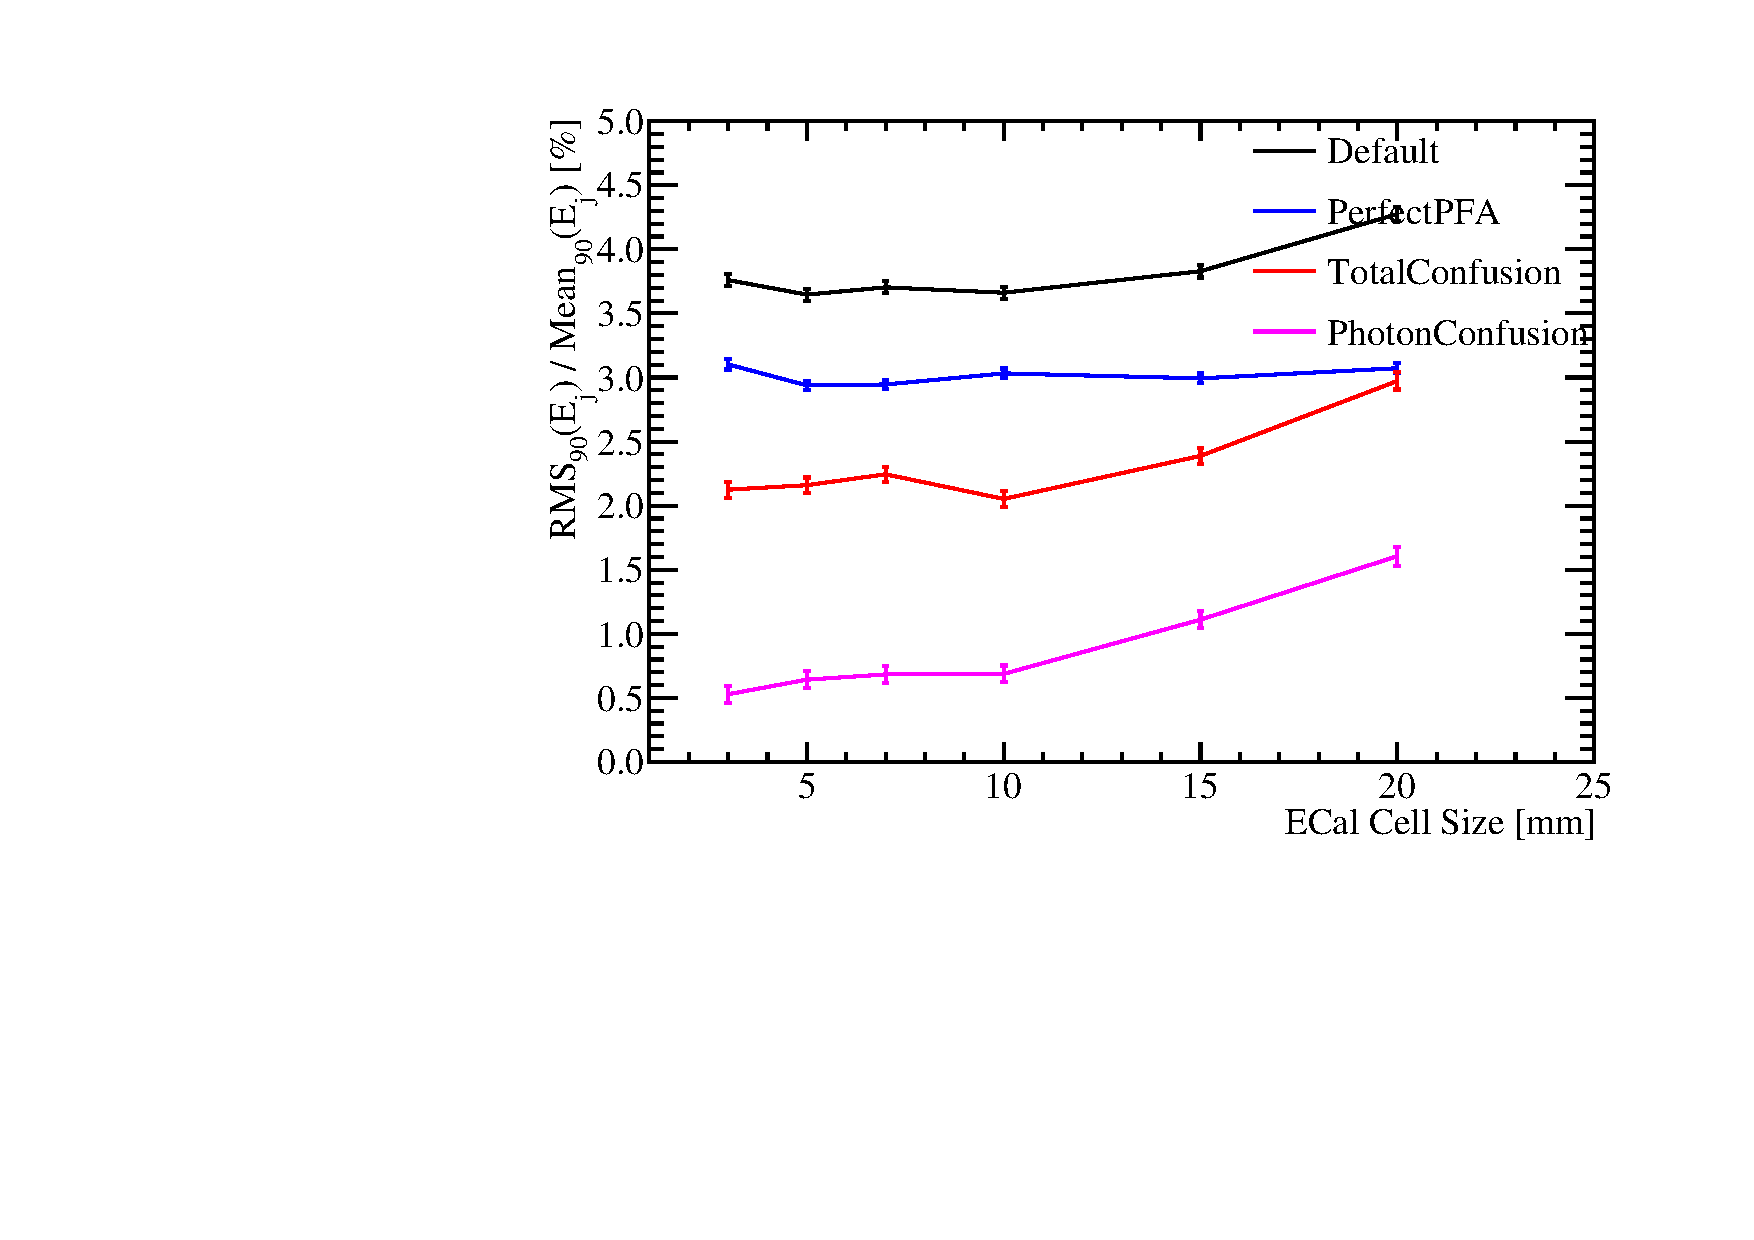
\includegraphics[width=0.5\textwidth]{OptimisationStudies/Plots/JetEnergyResolutions/JER_vs_SiliconECalCellSize_91GeV_DiJet_Breakdown.pdf}}
\subfloat[]{\label{fig:ecalsccellsize45break}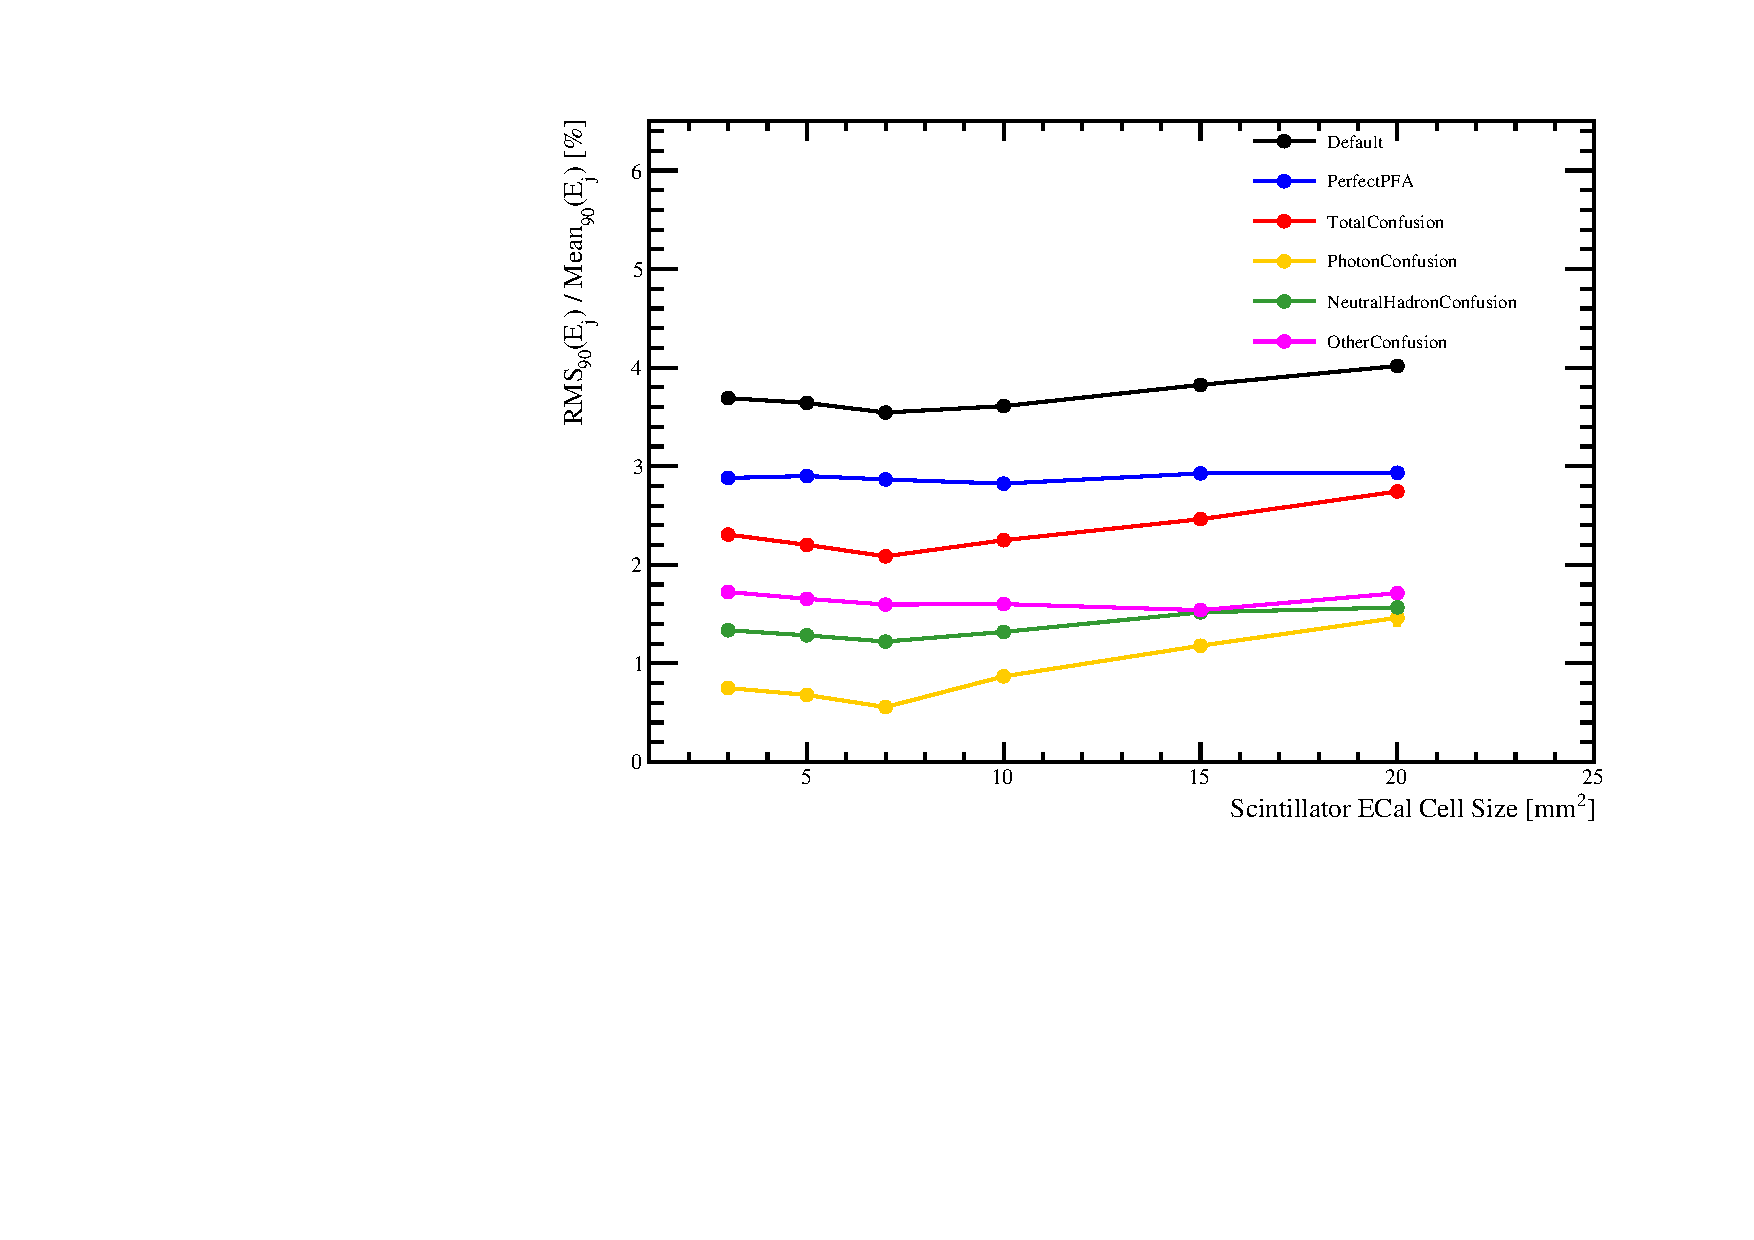
\includegraphics[width=0.5\textwidth]{OptimisationStudies/Plots/JetEnergyResolutions/JER_vs_ScintillatorECalCellSize_91GeV_DiJet_Breakdown.pdf}} \hfill
\subfloat[]{\label{fig:ecalsicellsize250break}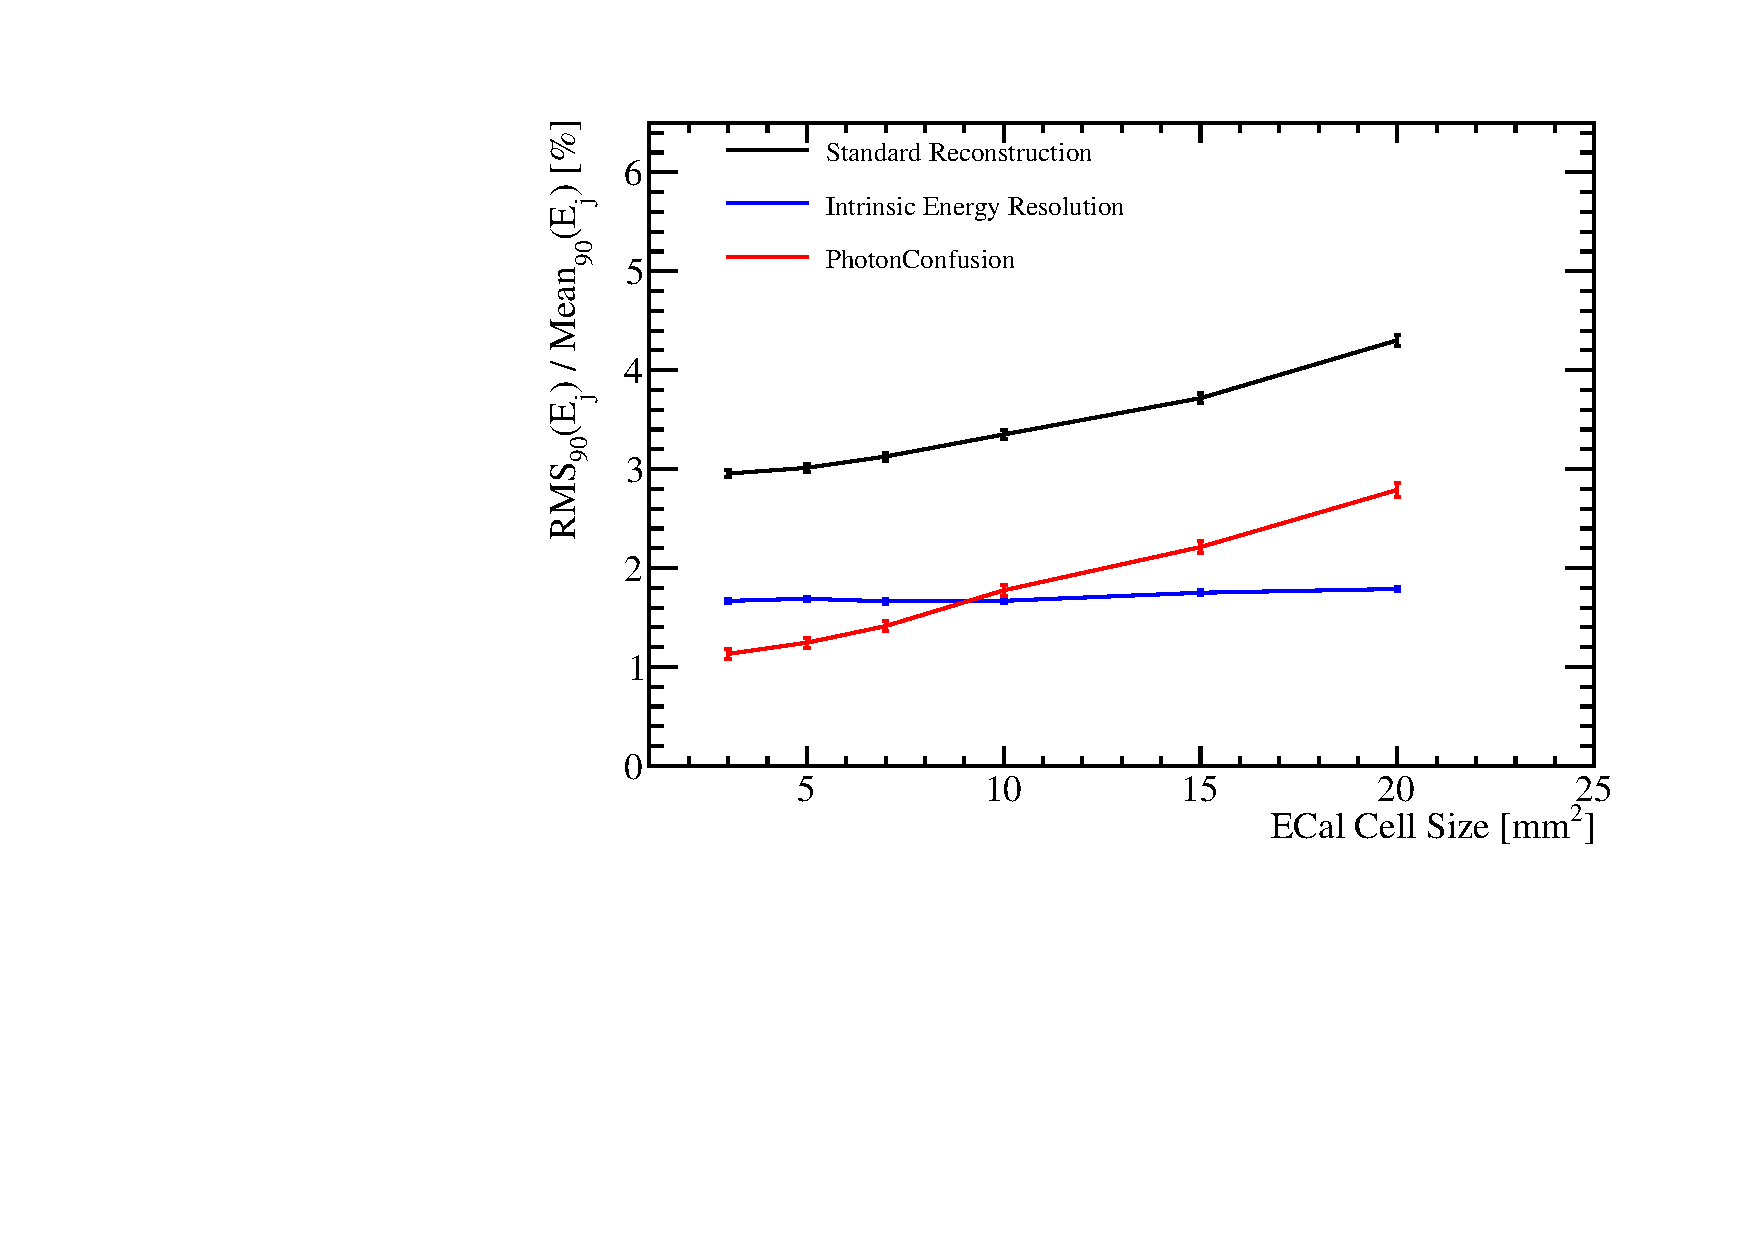
\includegraphics[width=0.5\textwidth]{OptimisationStudies/Plots/JetEnergyResolutions/JER_vs_SiliconECalCellSize_500GeV_DiJet_Breakdown.pdf}}
\subfloat[]{\label{fig:ecalsccellsize250break}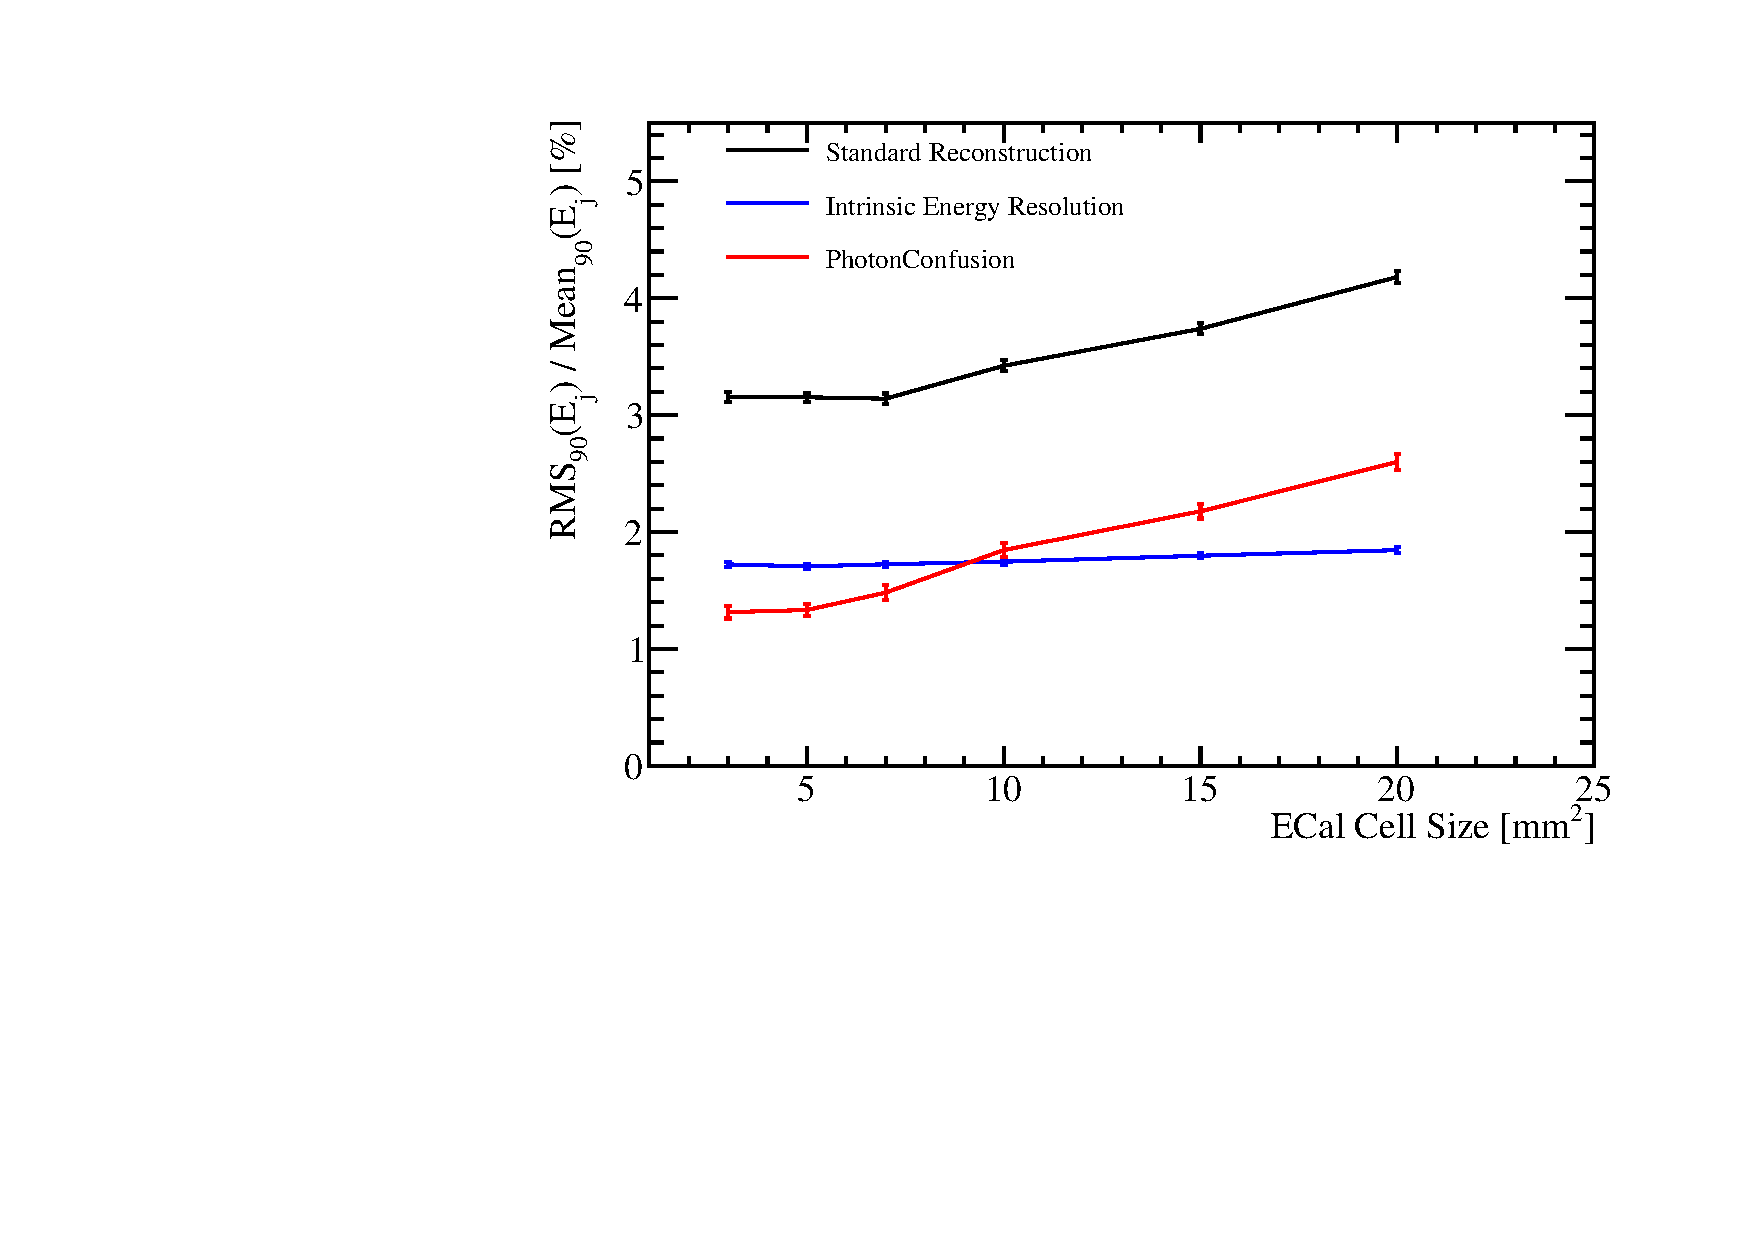
\includegraphics[width=0.5\textwidth]{OptimisationStudies/Plots/JetEnergyResolutions/JER_vs_ScintillatorECalCellSize_500GeV_DiJet_Breakdown.pdf}}
\caption[Contributions to the jet energy resolution shown as function of ECal cell size using the nominal ILD detector model for \protect\subref{fig:ecalsicellsize45break} the silicon ECal option and 45~GeV jets, \protect\subref{fig:ecalsccellsize45break} the scintillator ECal option and 45~GeV jets, \protect\subref{fig:ecalsicellsize250break} the silicon ECal option and 250~GeV jets and \protect\subref{fig:ecalsccellsize250break} the scintillator ECal option and 250~GeV jets.  The black curves correspond to the standard reconstruction, the blue curves to the intrinsic energy resolution contribution to the jet energy resolution, the red curves to the confusion contribution to the jet energy resolution and the magenta curves to the confusion contribution to the jet energy resolution related solely to photon reconstruction.]{Contributions to the jet energy resolution shown as function of ECal cell size using the nominal ILD detector model for \protect\subref{fig:ecalsicellsize45break} the silicon ECal option and 45~GeV jets, \protect\subref{fig:ecalsccellsize45break} the scintillator ECal option and 45~GeV jets, \protect\subref{fig:ecalsicellsize250break} the silicon ECal option and 250~GeV jets and \protect\subref{fig:ecalsccellsize250break} the scintillator ECal option and 250~GeV jets.  The black curves correspond to the standard reconstruction, the blue curves to the intrinsic energy resolution contribution to the jet energy resolution, the red curves to the confusion contribution to the jet energy resolution and the magenta curves to the confusion contribution to the jet energy resolution related solely to photon reconstruction}
\label{fig:ecalcellsizebreak}
\end{figure}

It is clear that the ECal cell size is extremely important for jet energy measurements, although it has little bearing on the intrinsic energy resolution of the ECal.  Separation of the hadronic decays of the W and Z bosons, i.e. $\sigma_{E}/E \lesssim 3.8\%$ \cite{arXiv:0907.3577}, can be achieved across the jet energy range considered here using a maximum ECal cell size of $15 \times 15 \text{ mm}^{2}$.  However, as reducing the ECal cell size further continues to benefit the jet energy resolution, minimising the ECal cell size is desirable.

%========================================================================================

\subsection{ECal Longitudinal Sampling Frequency} 
\label{sec:ecalnlayers}
The detector performance was simulated where the number of layers in the ECal was varied, while keeping the total material budget ($\text{X}_{0}$) approximately constant.  This study was performed for both the silicon and scintillator active material options.  In all cases tungsten was used for the ECal absorber material and the active layer thicknesses were not changed from those used in the nominal ILD ECal summarised in table \ref{table:defaultildecal}.  The different ECal layouts considered are summarised in table \ref{table:nlayersecaloption}.  

\begin{table}[h!]
\centering
\begin{tabular}{ r r r r r r}
\hline
Total Number & $N_{Layers}$ & Absorber & $N_{Layers}$ & Absorber & Total  \\
of Layers & Region 1 & Thickness & Region 2 & Thickness & Thickness \\
$N_{\text{Layers ECal}}$ & & Region 1 [mm] & &  Region 2 [mm] &  [$\text{X}_{0}$] \\
\hline
30 & 20 & 2.10 & 9 & 4.20 & 22.77 \\
26 & 17 & 2.40 & 8 & 4.80 & 22.60 \\
20 & 13 & 3.15 & 6 & 6.30 & 22.47 \\
16 & 10 & 4.00 & 5 & 8.00 & 22.31\\
\hline
\end{tabular}
\caption[The longitudinal structure of the ECal models considered in the optimisation study.  The radiation length of tungsten absorber is 3.504~mm \cite{Olive:2016xmw}.  Note that a presampler layer contributes one extra layer to the cumulative number of layers.]{The longitudinal structure of the ECal models considered in the optimisation study.  The radiation length of tungsten absorber is 3.504~mm \cite{Olive:2016xmw}.  Note that a presampler layer contributes one extra layer to the cumulative number of layers.}
\label{table:nlayersecaloption}
\end{table}

The energy resolution, for 100~GeV photons, as a function of the number of layers in the ECal is shown in figure \ref{fig:ecalsinlayers100gamma} for the silicon option and in figure \ref{fig:ecalscnlayers100gamma} for the scintillator option.  When the number of layers is increased $\sigma_{E}$/$E$ decreases, which is expected because the energy resolution for a sampling calorimeter is $\propto$ 1/$\sqrt{E \times N_{Layers}}$, where $E$ is the reconstructed energy and $N_{Layers}$ is the number of layers in the calorimeter.

\begin{figure}[h!]
\centering
\subfloat[]{\label{fig:ecalsinlayers100gamma}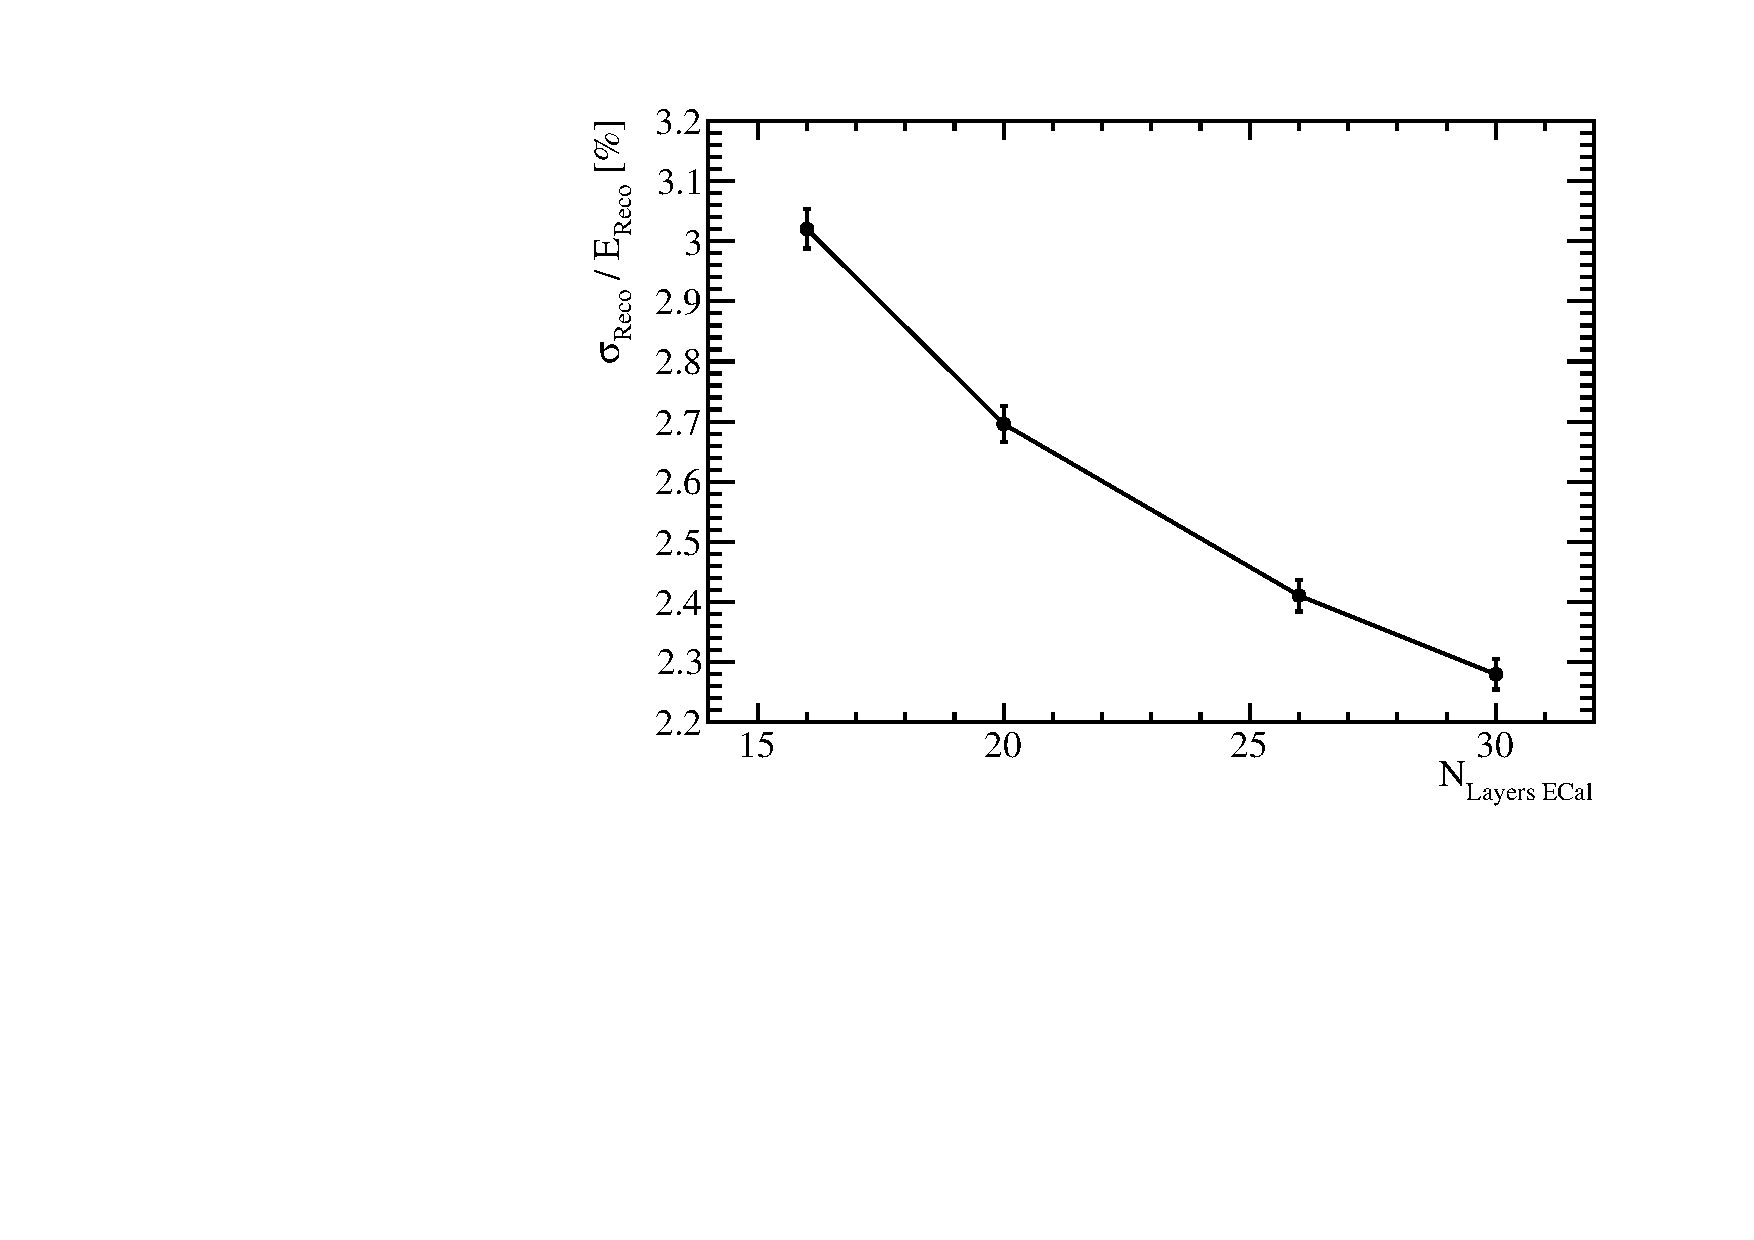
\includegraphics[width=0.5\textwidth]{OptimisationStudies/Plots/EnergyResolution/ER_vs_SiECalNLayers_100GeVPhoton.pdf}}
\subfloat[]{\label{fig:ecalscnlayers100gamma}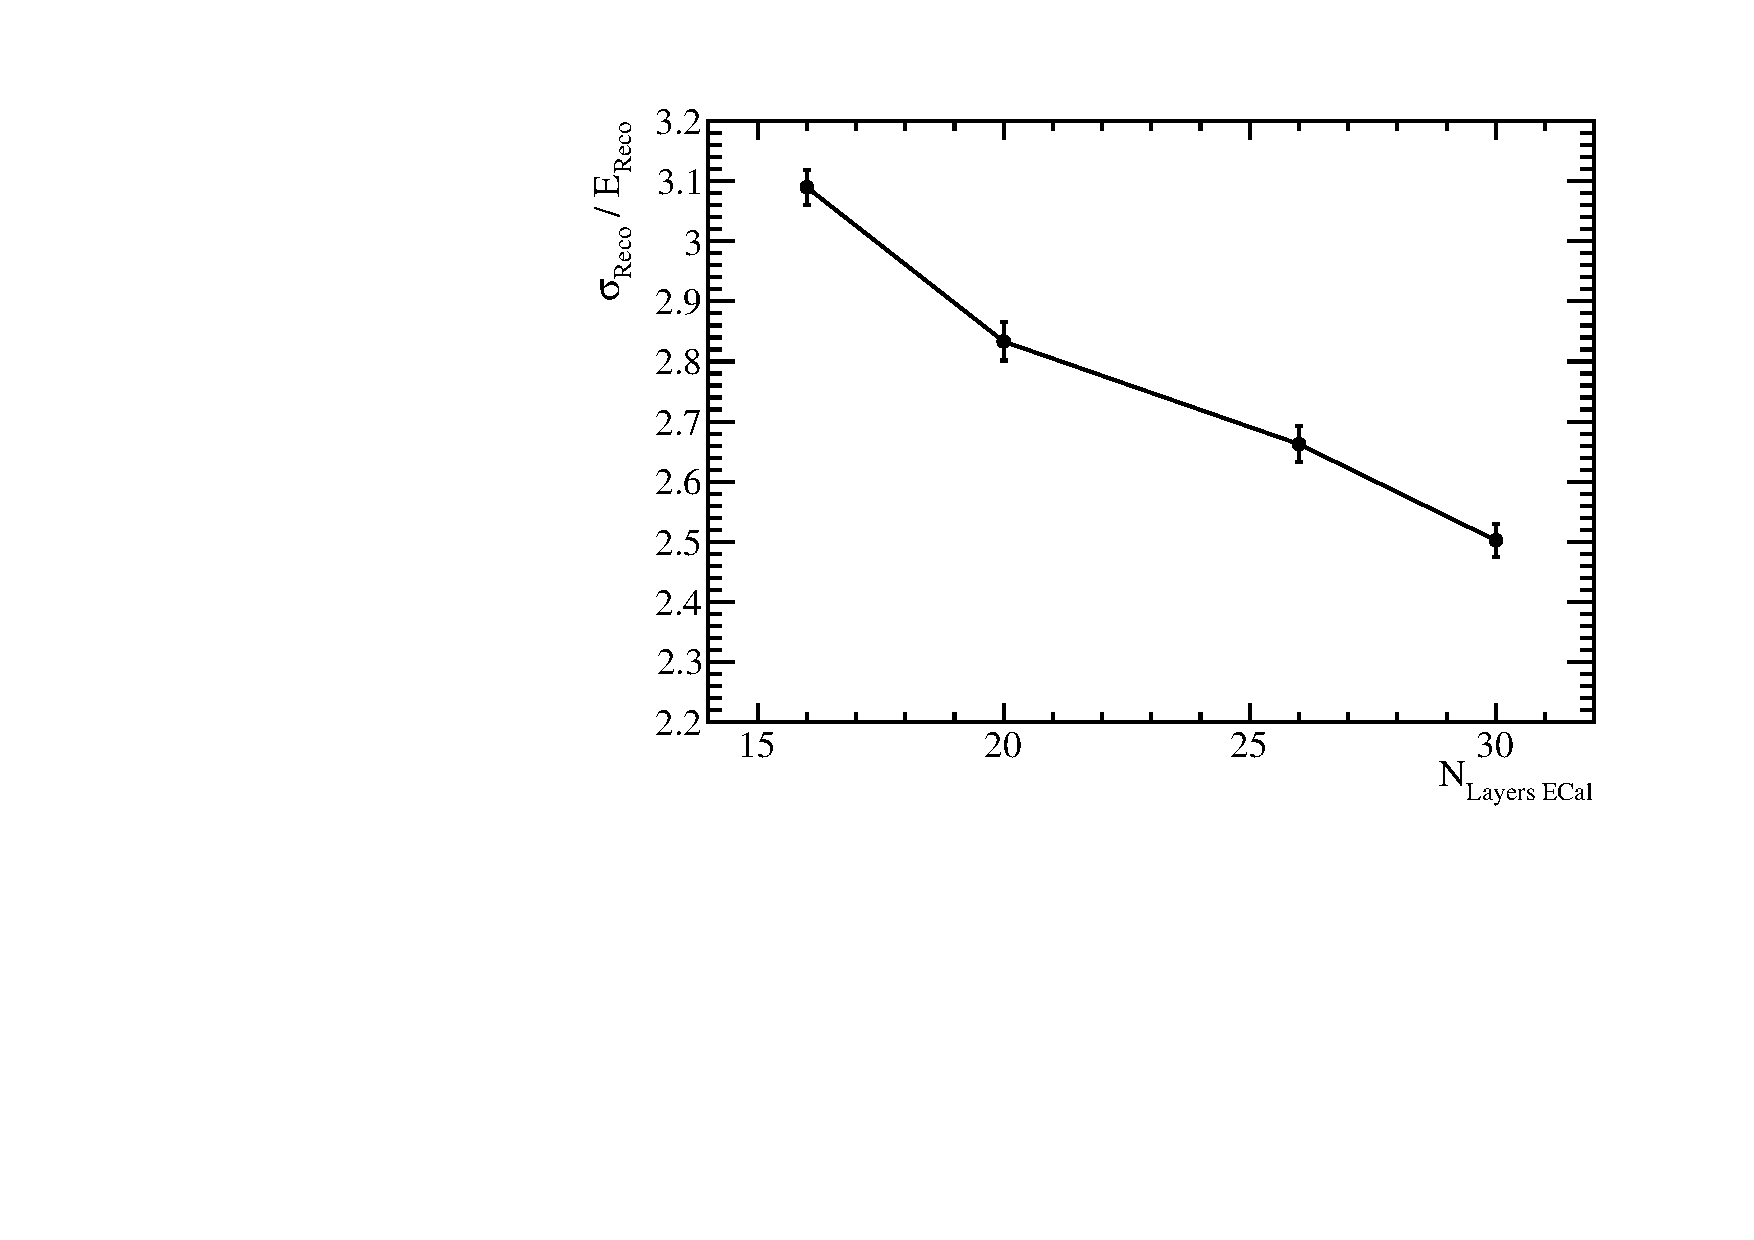
\includegraphics[width=0.5\textwidth]{OptimisationStudies/Plots/EnergyResolution/ER_vs_ScECalNLayers_100GeVPhoton.pdf}}
\caption[The energy resolution as a function of number of layers in the ECal for 100~GeV photons using the nominal ILD detector model with \protect\subref{fig:ecalsinlayers100gamma} the silicon and \protect\subref{fig:ecalscnlayers100gamma} the scintillator ECal option.]{The energy resolution as a function of number of layers in the ECal for 100~GeV photons using the nominal ILD detector model with \protect\subref{fig:ecalsinlayers100gamma} the silicon and \protect\subref{fig:ecalscnlayers100gamma} the scintillator ECal option.}
\label{fig:ecalnlayersgamma}
\end{figure}

When the number of layers in the ECal is increased, the intrinsic energy resolution benefits; the intrinsic energy resolution of the ECal improves by $\sim 25\%$ in both ECal options when increasing the number of layers from 16 to 30.  This has the knock-on effect of reducing the confusion contribution to the jet energy resolution, which can be seen in figures \ref{fig:ecalsinlayers} and \ref{fig:ecalscnlayers} for the silicon and scintillator ECal options\textcolor{blue}{,} respectively.  In both cases, the jet energy resolution was found to improve when the number of layers in the ECal was increased; the jet energy resolution goes from $\sim 4.4$ to $\sim 3.6\%$ for the silicon option and from $\sim 4.1$ to $\sim 3.6\%$ for the scintillator option when increasing the number of layers from 16 to 30.  The magnitude of the change in jet energy resolution is dependent upon the jet energy, with a stronger dependancy being observed for low energy jets.  This is expected from the stochastic contribution to the energy resolution for a sampling calorimeter.  For high jet energies, changing the number of layers in the ECal does not significantly affect the jet energy resolution because the jet energy resolution is dominated by confusion.  For low jet energies, the stochastic contribution to the energy resolution is bigger making it possible to resolve the changes to it when varying the number of layers in the ECal.  

The decomposition of the jet energy resolution into the intrinsic energy resolution and confusion contributions for 45 and 250~GeV jets are shown, for both the silicon and scintillator ECal options, in figure \ref{fig:ecalnlayersbreak}.  As expected, the improvement to the intrinsic energy resolution seen when increasing the number of layers in the ECal leads to the knock-on effect of lowering the confusion.  However, significantly the magnitude of the change to the intrinsic energy resolution and confusion contributions to the jet energy resolution when varying the number of layers in the ECal are comparable in size.  This shows that pattern recognition is as important for detector performance in the particle flow paradigm \textcolor{blue}{as} intrinsic energy resolution.  

\begin{figure}[h!]
\centering
\subfloat[]{\label{fig:ecalsinlayers}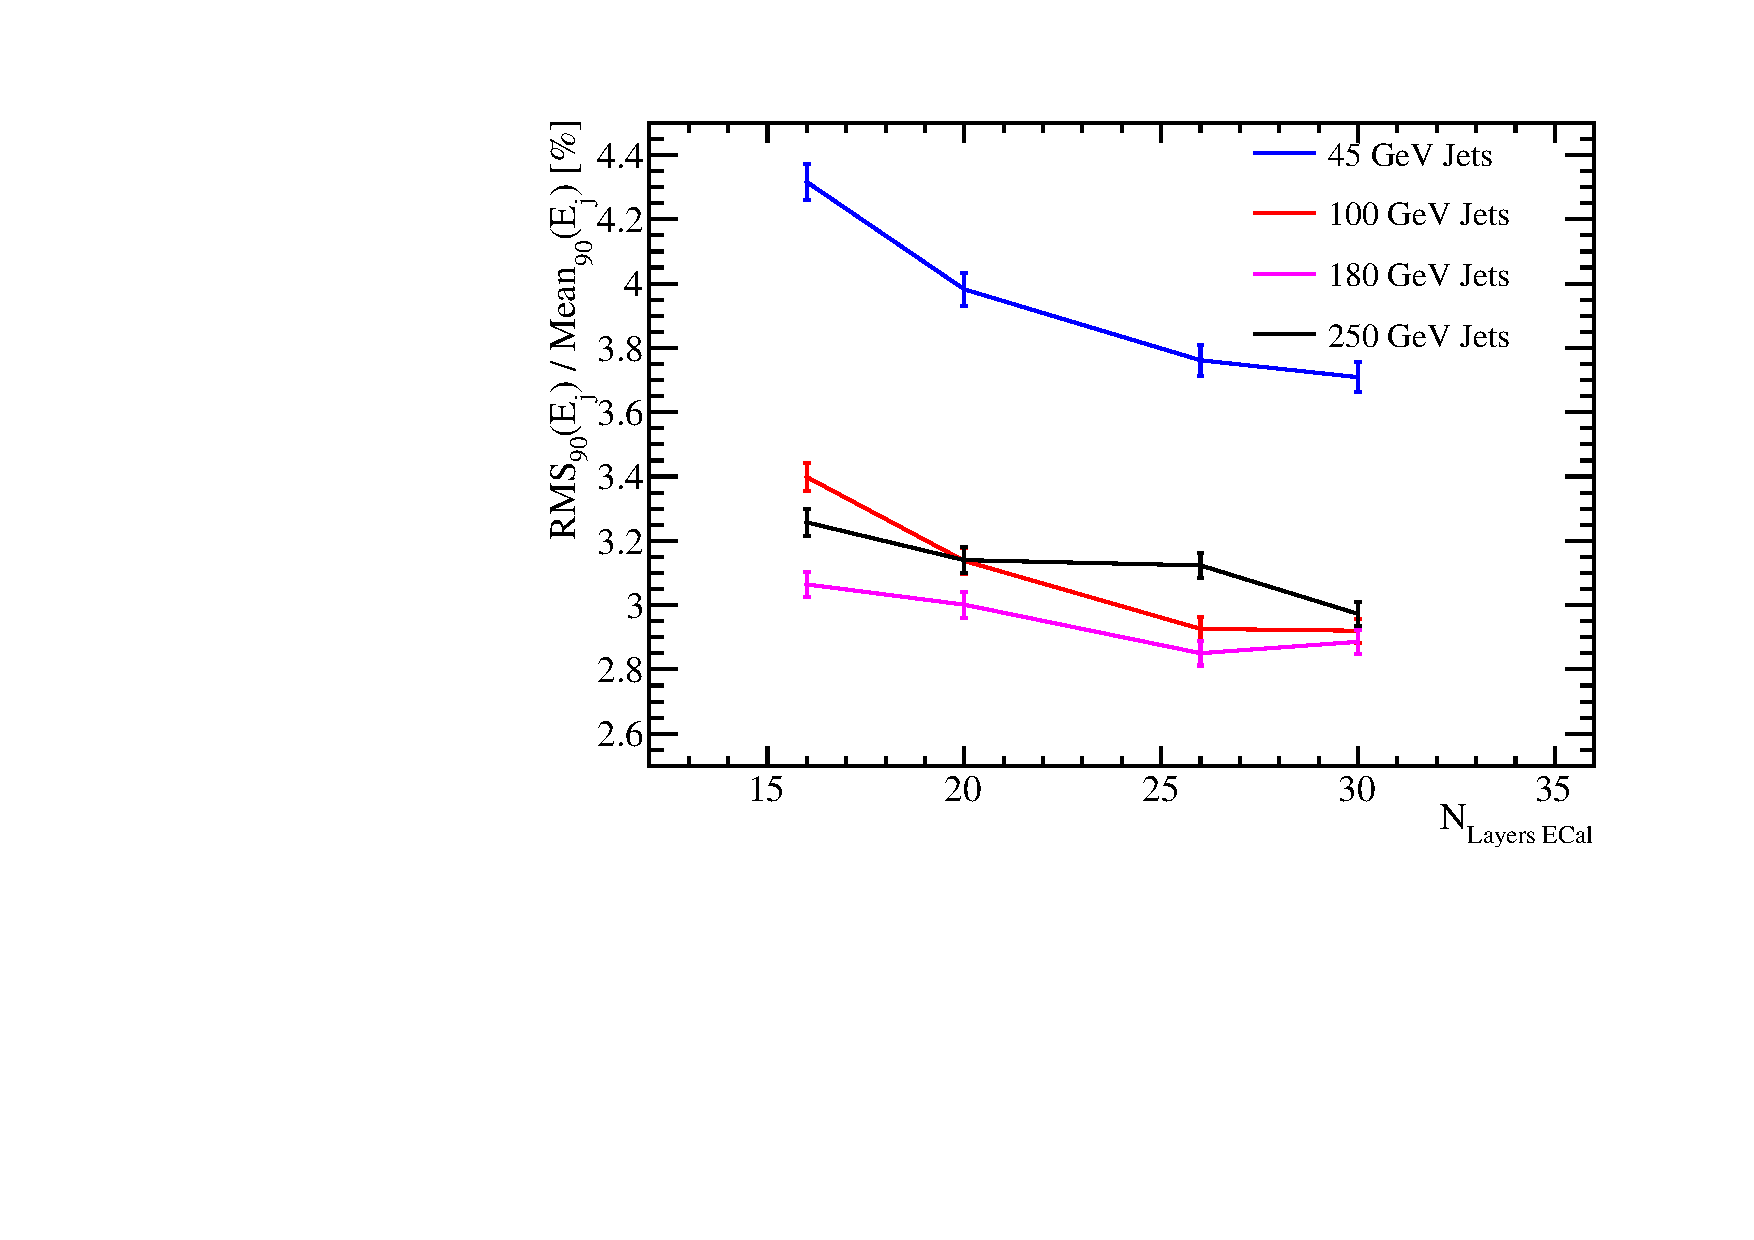
\includegraphics[width=0.5\textwidth]{OptimisationStudies/Plots/JetEnergyResolutions/JER_vs_SiliconECalNumberofLayers.pdf}}
\subfloat[]{\label{fig:ecalscnlayers}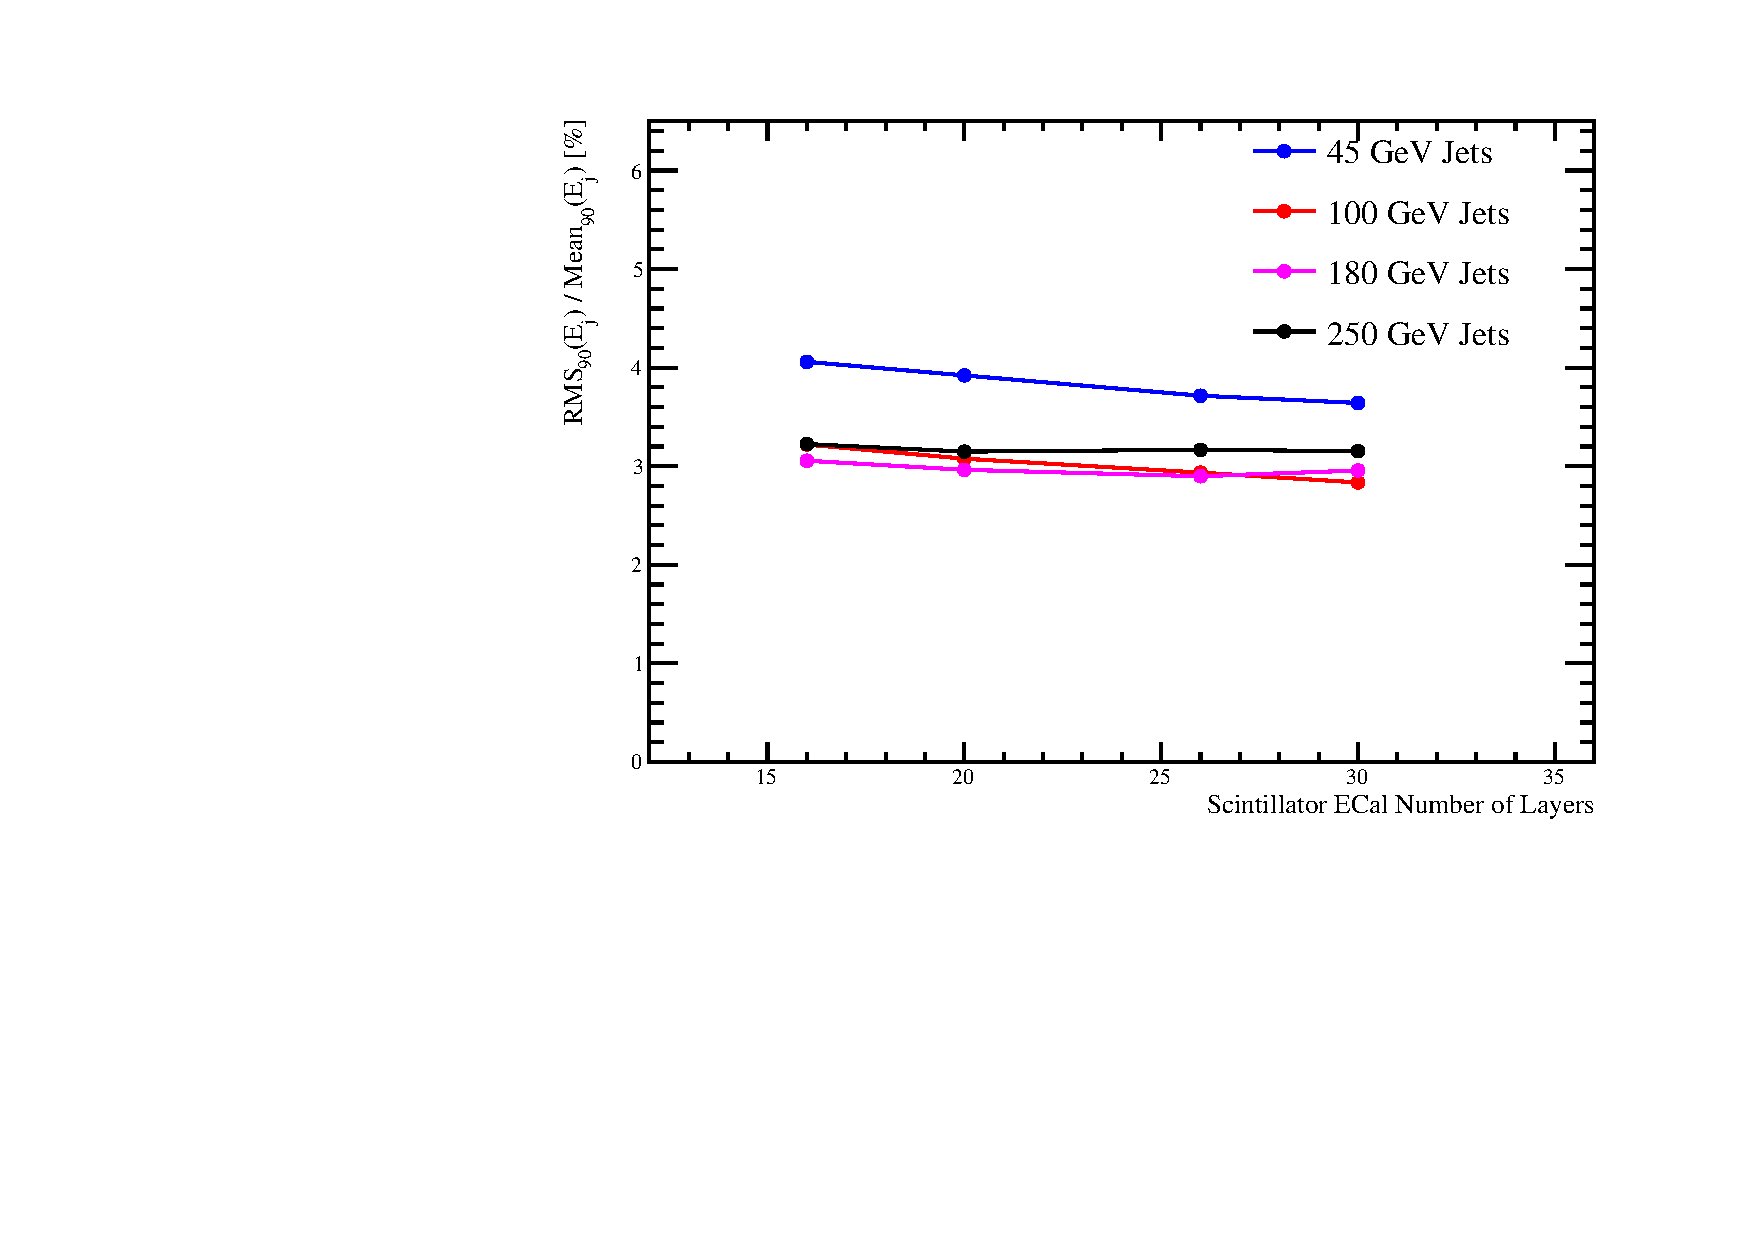
\includegraphics[width=0.5\textwidth]{OptimisationStudies/Plots/JetEnergyResolutions/JER_vs_ScintillatorECalNumberofLayers.pdf}} \hfill
\caption[The jet energy resolution as a function of number of layers in the ECal for various jet energies using the nominal ILD detector model with \protect\subref{fig:ecalsinlayers} the silicon and \protect\subref{fig:ecalscnlayers} the scintillator ECal option.]{The jet energy resolution as a function of number of layers in the ECal for various jet energies using the nominal ILD detector model with \protect\subref{fig:ecalsinlayers} the silicon and \protect\subref{fig:ecalscnlayers} the scintillator ECal option.}
\label{fig:ecalnlayers}
\end{figure}

\begin{figure}[h!]
\centering
\subfloat[]{\label{fig:ecalsinlayers45break}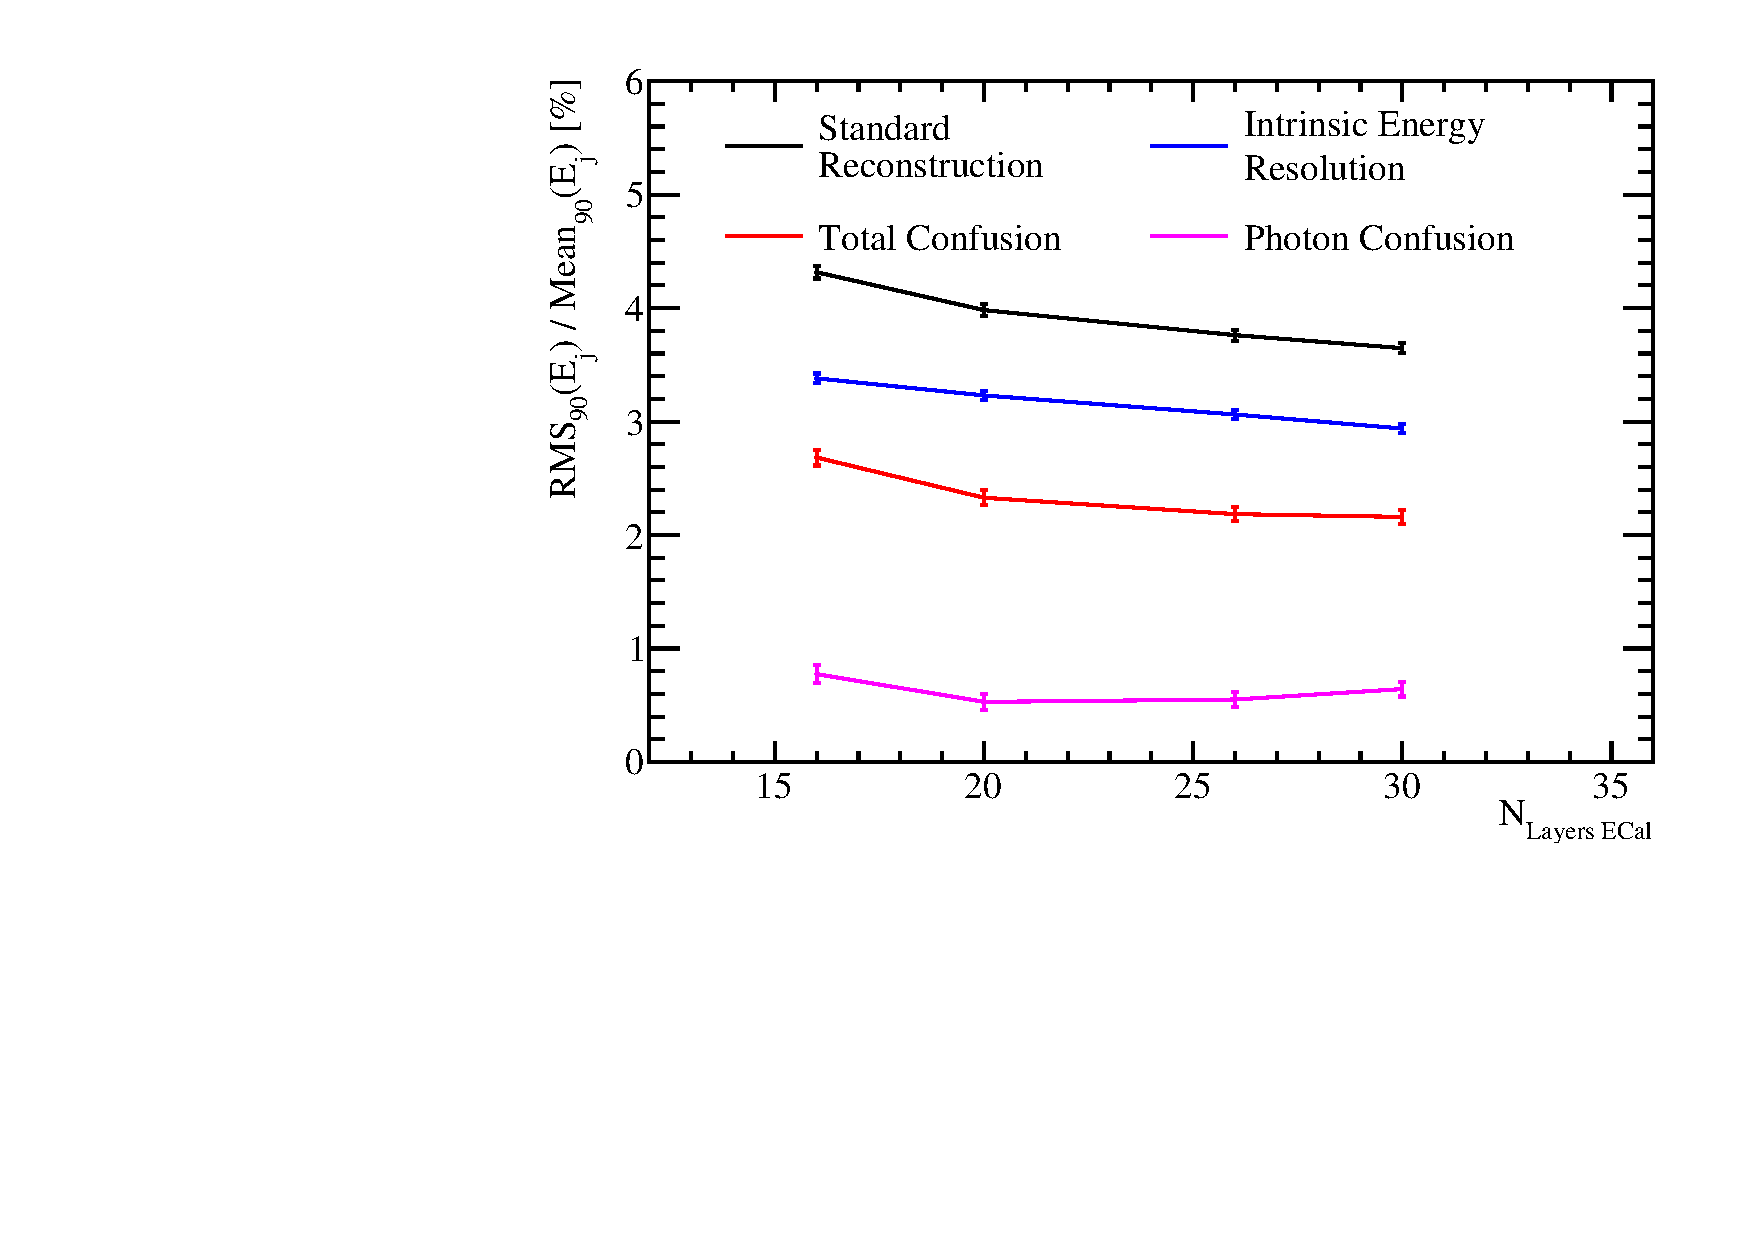
\includegraphics[width=0.5\textwidth]{OptimisationStudies/Plots/JetEnergyResolutions/JER_vs_SiliconECalNumberofLayers_91GeV_DiJet_Breakdown.pdf}}
\subfloat[]{\label{fig:ecalscnlayers45break}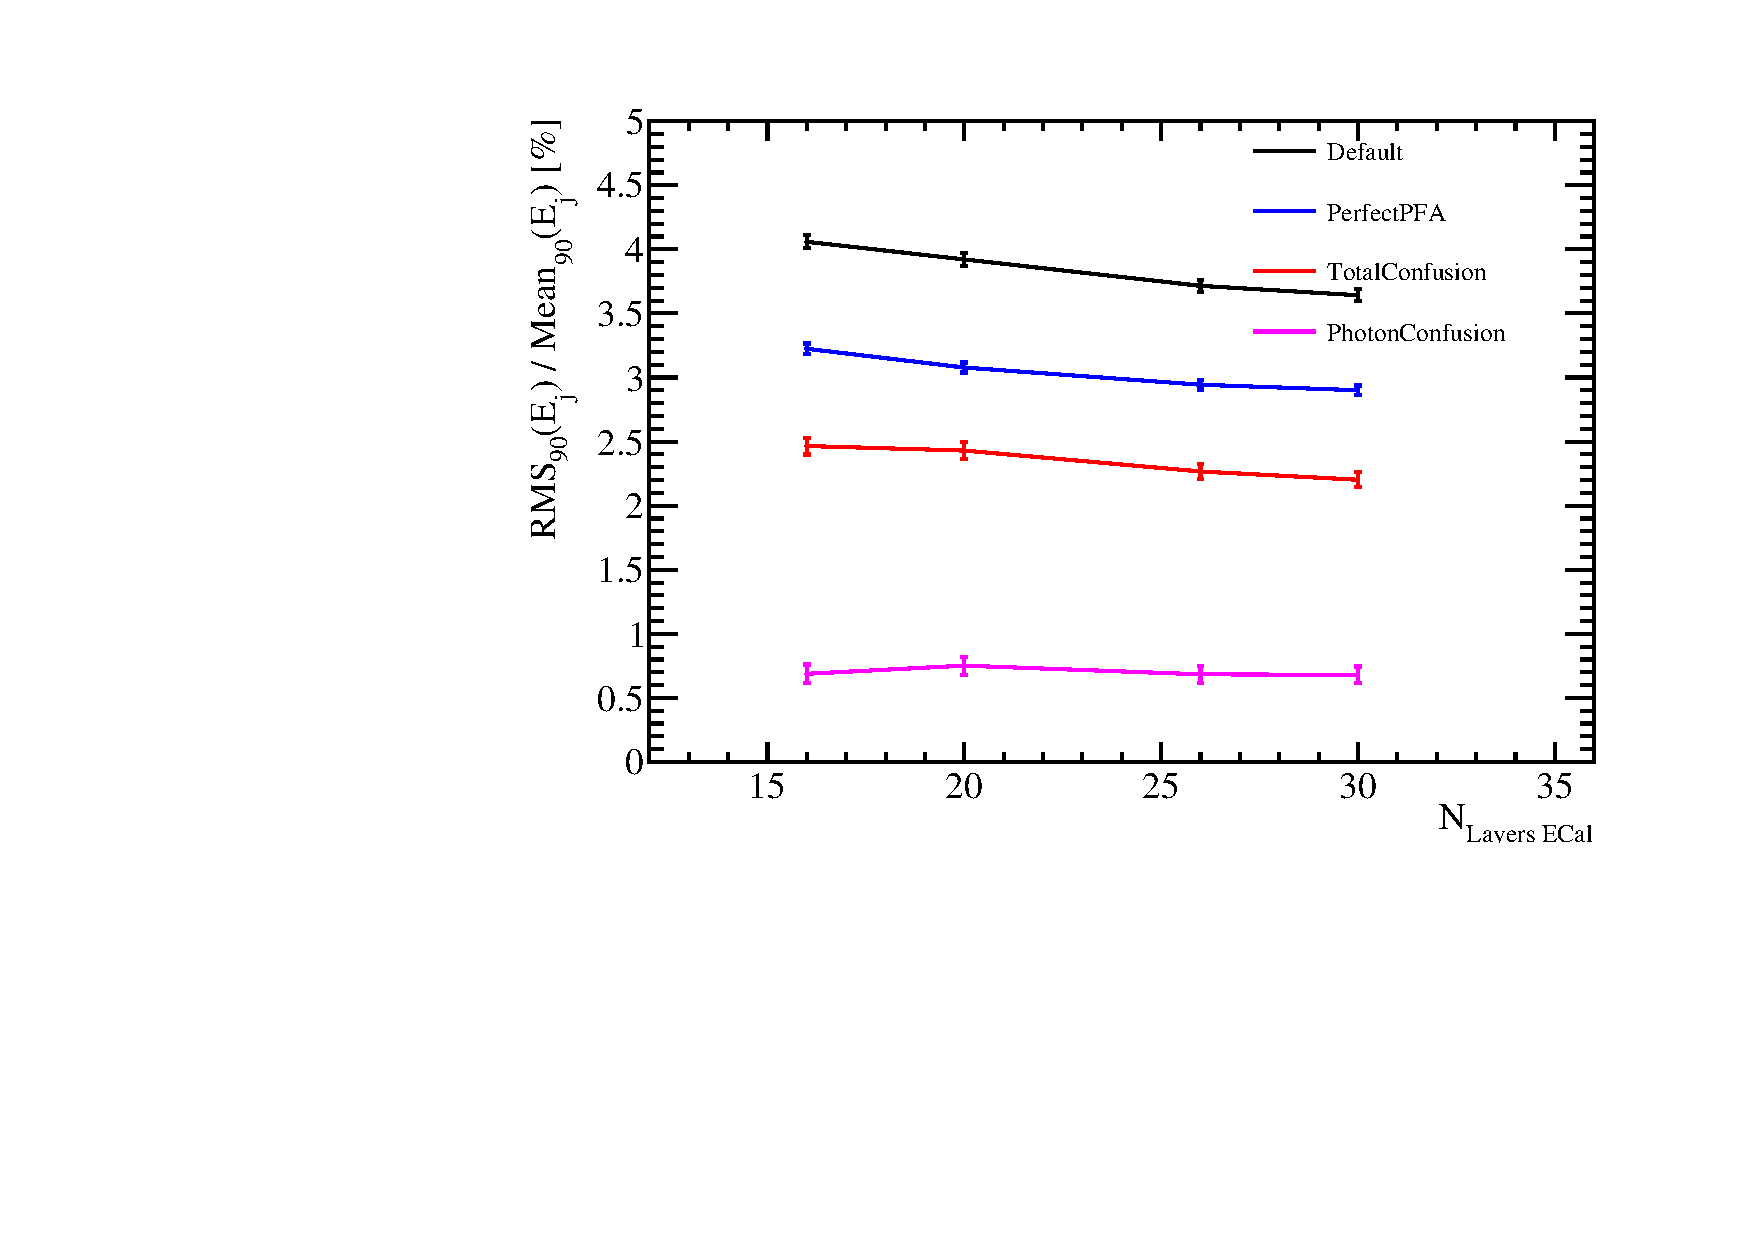
\includegraphics[width=0.5\textwidth]{OptimisationStudies/Plots/JetEnergyResolutions/JER_vs_ScintillatorECalNumberofLayers_91GeV_DiJet_Breakdown.pdf}} \hfill
\subfloat[]{\label{fig:ecalsinlayers250break}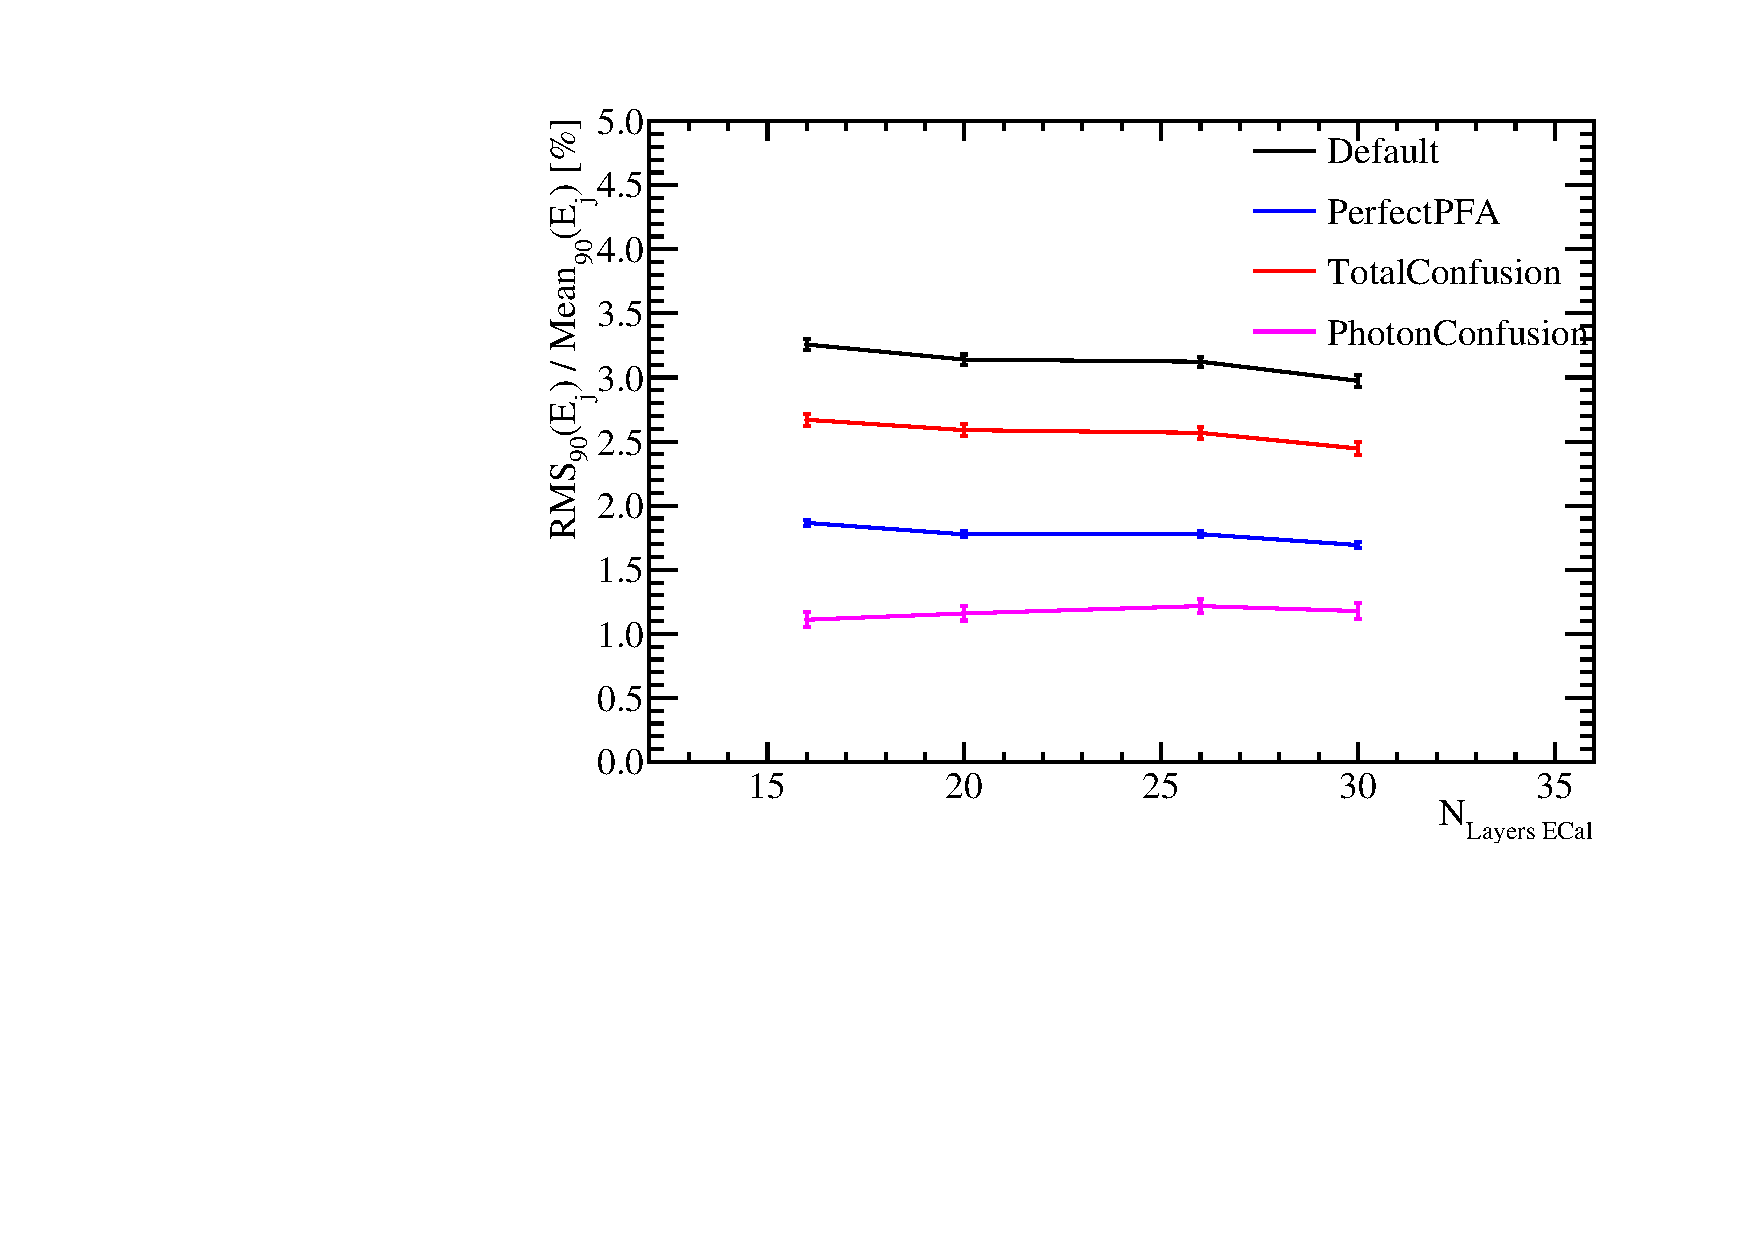
\includegraphics[width=0.5\textwidth]{OptimisationStudies/Plots/JetEnergyResolutions/JER_vs_SiliconECalNumberofLayers_500GeV_DiJet_Breakdown.pdf}}
\subfloat[]{\label{fig:ecalscnlayers250break}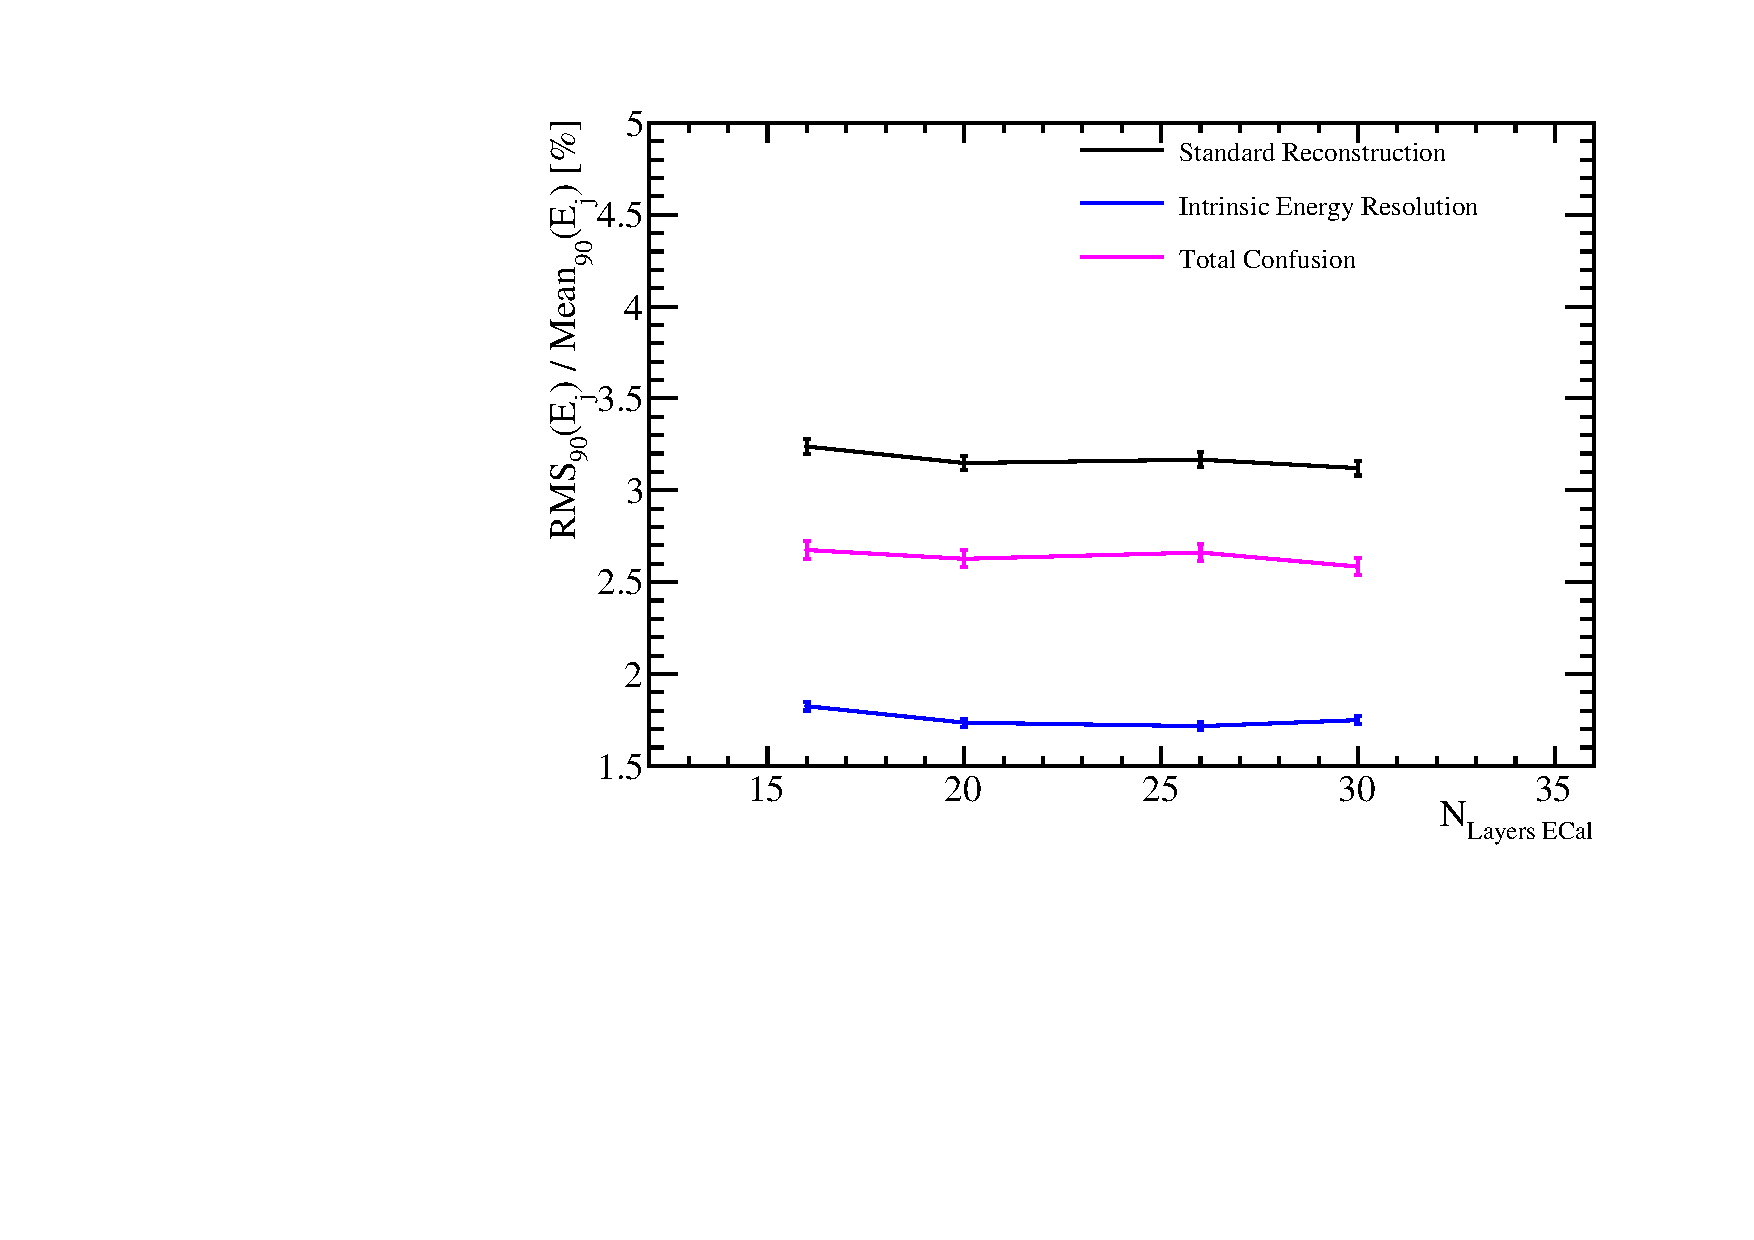
\includegraphics[width=0.5\textwidth]{OptimisationStudies/Plots/JetEnergyResolutions/JER_vs_ScintillatorECalNumberofLayers_500GeV_DiJet_Breakdown.pdf}}
\caption[Contributions to the jet energy resolution shown as function of number of layers in the ECal using the nominal ILD detector model for \protect\subref{fig:ecalsinlayers45break} the silicon ECal option and 45~GeV jets, \protect\subref{fig:ecalscnlayers45break} the scintillator ECal option and 45~GeV jets, \protect\subref{fig:ecalsinlayers250break} the silicon ECal option and 250~GeV jets and \protect\subref{fig:ecalscnlayers250break} the scintillator ECal option and 250~GeV jets.  The black curves correspond to the standard reconstruction, the blue curves to the intrinsic energy resolution contribution to the jet energy resolution, the red curves to the confusion contribution to the jet energy resolution and the magenta curves to the confusion contribution to the jet energy resolution related solely to photon reconstruction.]{Contributions to the jet energy resolution shown as function of number of layers in the ECal using the nominal ILD detector model for \protect\subref{fig:ecalsinlayers45break} the silicon ECal option and 45~GeV jets, \protect\subref{fig:ecalscnlayers45break} the scintillator ECal option and 45~GeV jets, \protect\subref{fig:ecalsinlayers250break} the silicon ECal option and 250~GeV jets and \protect\subref{fig:ecalscnlayers250break} the scintillator ECal option and 250~GeV jets.  The black curves correspond to the standard reconstruction, the blue curves to the intrinsic energy resolution contribution to the jet energy resolution, the red curves to the confusion contribution to the jet energy resolution and the magenta curves to the confusion contribution to the jet energy resolution related solely to photon reconstruction.}
\label{fig:ecalnlayersbreak}
\end{figure}

%========================================================================================

\subsection{ECal Active Material}
In sections \ref{sec:ecalcells} and \ref{sec:ecalnlayers} the performance of the ECal was reported for both the silicon and scintillator options and to a large extent the performance of the two options was similar, but not identical:

\begin{itemize}
\item The intrinsic energy resolution of the silicon ECal option is better than that of the scintillator option at very high energies.  For 500~GeV photons the intrinsic energy resolution is $\sim 25\%$ better for the silicon option.  Section \ref{sec:nominaldetectorperformance} contains a comparison between the photon energy resolution for the two ECal options, which clearly illustrates this.  The most likely origin of the differing energy resolutions is the implementation of Birks' law \cite{Birks:1951boa} for scintillator active materials, which states
%
\begin{equation}
d\mathcal{L}/dx \propto \frac{dE/dx}{1+k_{B}dE/dx}\text{ ,}
\end{equation}
%
\noindent where $d\mathcal{L}/dx$ is the scintillation light yield per unit path length, $dE/dx$ is the energy deposited per unit path length and $k_{B}$ is a material property constant.  For large energy deposits per unit length, such as those found in high energy photons, the light yield saturates causing a degradation in the energy resolution.  When comparing the photon energy resolution for the silicon and scintillator ILD ECal options, which can be found in section \ref{sec:nominaldetectorperformance}, the saturation effect starts to degrade the energy resolution for the scintillator option \textcolor{blue}{for photons of energy $\gtrsim$ 50~GeV}.  
\item The "dead" region due to the presence of the MPPC in the simulation of the scintillator ECal option degrades performance of the detector for small transverse granularities, see figure \ref{fig:ecalcellsizegamma}.
\end{itemize}

In summary, the performance of the two options, in terms of energy and jet energy resolution, at ILC-like energies is comparable.  However, the silicon option is preferred when manufacture and implementation of the two models is compared.  While constructing silicon wafers to fit a $5 \times 5 \text{ mm}^{2}$ square cell size is achievable, this would be extremely challenging for scintillator tiles.  To resolve this in actuality, the scintillator ECal option would have to use $5 \times 45 \text{ mm}^{2}$ scintillator strips that are arranged in alternating directions in each ECal layer \cite{Behnke:2013lya}.  By combining information from neighbouring layers it becomes possible to approach an effective $5 \times 5 \text{ mm}^{2}$ square cell size.  

%========================================================================================
%========================================================================================

\section{Hadronic Calorimeter Optimisation}
\label{sec:hcal}
The purpose of \textcolor{blue}{a hadronic} calorimeter (HCal) is to measure the energy deposits from hadronic showers.  The HCal in the default ILD detector model, summarised in table \ref{table:defaultildhcal}, is approximately 6 nuclear interaction lengths ($\lambda_{I}$) deep.  The ECal contributes approximately one $\lambda_{I}$ giving a total of $\approx 7 \lambda_{I}$, which is sufficient to contain jets at ILC like energies.  The longitudinal structure of this model consists of 48 readout layers each containing a 3~mm active layer of scintillator and a 20~mm absorber layer of iron.  

\begin{table}[h!]
\centering
\begin{tabular}{ l l}
\hline
Parameter & Default Value \\
\hline
Cell Size & $30 \times 30 \text{ mm}^{2}$ square cells \\
Number of Layers & 48 readout layers \\
Active Material Choice & Scintillator \\
Active Material Thickness & 3 mm  \\
Absorber Material Choice & Steel \\
Absorber Material Thickness & 20 mm \\
\hline
\end{tabular}
\caption[The configuration of the HCal in the nominal ILD detector model \cite{Behnke:2013lya}.]{The configuration of the HCal in the nominal ILD detector model \cite{Behnke:2013lya}.}
\label{table:defaultildhcal}
\end{table}
% Nuclear interaction length iron 167.7mm
% Nuclear interaction length tungsten 99.46mm 
% Nuclear interaction length silicon 465.2mm 
% Nuclear interaction length polystyrene 770.7mm

There are several readout approaches under consideration for the HCal including fully analogue, fully digital and semi-digital.  Analogue readout reports the energy within each HCal cell using a continuous variable, while digital readout only produces a response if the energy deposited within a calorimeter cell is above a given threshold.  The semi-digital approach mirrors that of the digital approach, but has three responses each with a different energy threshold.  While the energy resolution for digital calorimeters is not as good as that of analogue calorimeters, it is possible to construct smaller cell sizes using a digital readout.  In traditional calorimetry, a digital calorimeter would give a worse jet energy resolution than the analogue equivalent, however, that is not necessarily the case in particle flow calorimetry.  If a digital calorimeter could be realised with a much \textcolor{blue}{smaller} cell size than the analogue equivalent, then the \textcolor{blue}{effect} of confusion in the digital calorimeter may be reduced such that it compensates for any loss to intrinsic energy resolution.  In the following studies only the optimisation of the analogue HCal is presented as this is the readout approach used in the nominal ILD detector model.  

A number of options were simulated where the following parameters in the HCal were varied:
\begin{itemize}
\item Cell size:  This is crucial for successful application \textcolor{blue}{of} particle flow calorimetry for making associations between clusters of calorimeter hits and charged particle tracks.  It is expected that the intrinsic energy resolution be invariant to changes in the HCal cell size.  
\item Number of readout layers:  The number of layers in the HCal are varied, however, the thickness of those layers match those of the nominal ILD HCal design.  This means the total depth of the HCal in $\lambda_{I}$ is changing.  It is expected that this study will determine the effect of leakage of energy out of the back of the HCal.
\item Longitudinal sampling frequency:   This involves changing the number of readout layers in the HCal while simultaneously changing the thicknesses of the active and absorber layers to keep the total number of $\lambda_{I}$ in the HCal constant.  As this modifies the sampling of particle showers in the HCal, it will affect the intrinsic energy resolution of the HCal.
\item Sampling fraction:  This is the ratio of the active medium thickness to the absorber medium thickness.  This controls how particle showers within the calorimeter are sampled.  In this study the total depth of the HCal in $\lambda_{I}$ is held constant between detector models.  
\item Absorber material choice:  Two options have been considered: steel and tungsten.  This choice affects the growth and propagation of hadronic showers.  
\end{itemize}

%========================================================================================

\subsection{HCal Cell Size}
\label{sec:hcalcells}
The HCal cell size is an important detector parameter in the application of particle flow calorimetry.  Smaller HCal cell sizes will lead to a finer spatial resolution that can be used to better separate charged and neutral particle calorimetric energy deposits.  On the other hand, this will also lead to an increase in the number of readout channels that will raise the cost of the calorimeter.  Therefore, it is highly desirable to achieve the optimal physics performance using the largest cell size possible.  The nominal ILD HCal has a 30~mm square cell size and in this study the following cell sizes were considered; $10 \times 10 \text{ mm}^{2}$, $20 \times 20 \text{ mm}^{2}$, $30 \times 30 \text{ mm}^{2}$, $40 \times 40 \text{ mm}^{2}$, $50 \times 50 \text{ mm}^{2}$ and $100 \times 100 \text{ mm}^{2}$.  

In the nominal ILD detector, 50~GeV long-lived neutral kaons ($\text{K}^{0}_{L}$s) will deposit $\sim 65\%$ of their energy in the HCal and $\sim 35\%$ in the ECal.  As 50~GeV $\text{K}^{0}_{L}$s deposit the bulk of their energy in the HCal, they are appropriate to use when determining the performance of the HCal.  However, it should be emphasised that the $\text{K}^{0}_{L}$ energy resolutions represent the intrinsic energy resolution of the whole ILD detector and not purely that of the HCal.  

Figure \ref{fig:hcalcellser} shows the energy resolution for 50~GeV $\text{K}^{0}_{L}$s as a function of cell size.  As expected, the hadronic energy resolution does not strongly depend on the HCal cell size.  The only statistically significant variation in energy resolution is observed for the $100 \times 100 \text{ mm}^{2}$ HCal cell size.  For this model the energy resolution gets worse by $\sim8\%$ in comparison to the other models considered.  The most likely cause of this is a reduction in the effectiveness of the HCal hit energy truncation, which is described in section \ref{sec:hcalcelltruncation}.  The reduced effectiveness is expected because the precision used when obtaining the optimal energy truncation becomes worse as HCal cell size diverges from the nominal value.  

\begin{figure}[h!]
\centering
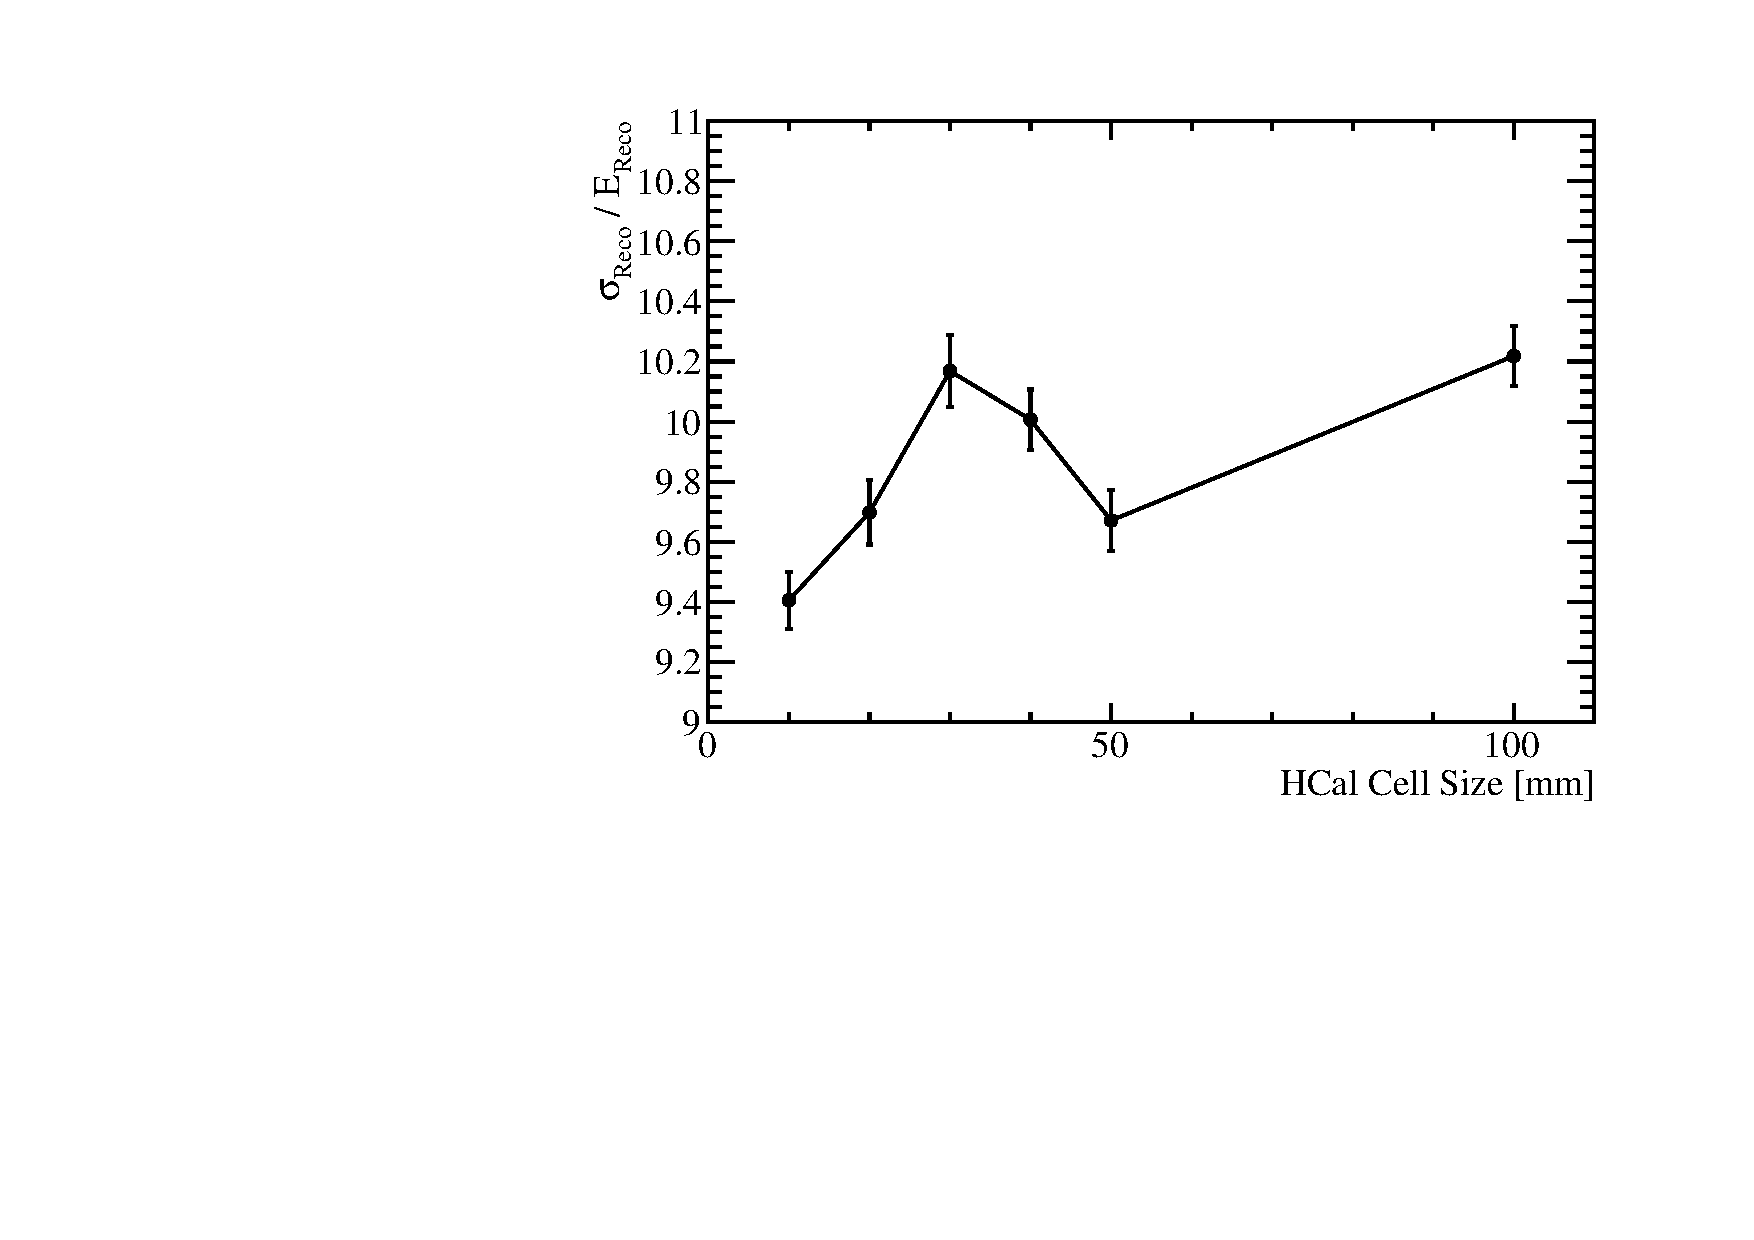
\includegraphics[width=0.5\textwidth]{OptimisationStudies/Plots/EnergyResolution/ER_vs_HCalCellSize_50GeVKaon0L.pdf}
\caption[The energy resolution as a function of HCal cell size for 50~GeV $\text{K}^{0}_{L}$ events using the nominal ILD detector model.]{The energy resolution as a function of HCal cell size for 50~GeV $\text{K}^{0}_{L}$ events using the nominal ILD detector model.}
\label{fig:hcalcellser}
\end{figure}

A smaller HCal cell size will lead to better separation of charged and neutral hadron calorimetric energy deposits, therefore, it is expected that the confusion contribution to the jet energy resolution will be reduced by using smaller HCal cell sizes.  Figure \ref{fig:hcalcellsize} shows the jet energy resolution as a function of cell size in the HCal.  At low jet energies there is no strong dependency of the jet energy resolution on the HCal cell size, which is as expected from the $\text{K}^{0}_{L}$ energy resolution study.  For high energy jets there is a clear dependence, with lower HCal cell sizes leading to better jet energy resolutions; the jet energy resolution for 250~GeV jets goes from $\sim 2.7\%$ to $\sim 3.5\%$ when the HCal cell size is increased from $10 \times 10 \text{ mm}^{2}$ to $100 \times 100 \text{ mm}^{2}$.  Examining the different contributions to the jet energy resolution, shown in figure \ref{fig:hcalcellsizebreak} it can be seen that the intrinsic energy resolution contribution does not depend on the HCal cell size; it is the confusion contribution that drives the overall trend in the jet energy resolution.  This is particularly clear at high jet energies where the confusion contribution to the jet energy resolution dominates that of the intrinsic energy resolution contribution.  At high jet energies smaller HCal cell sizes leads to a reduction in the effect of confusion; the confusion contribution to the jet energy resolution is reduced by $\sim 25\%$ when reducing the HCal cell size from $100 \times 100 \text{ mm}^{2}$ to $10 \times 10 \text{ mm}^{2}$.  At low jet energies the trend is less clear, as the confusion contribution is less dominant.  Nevertheless, a reduction in the effect of confusion with decreasing cell size is still visible for all but the smallest HCal cell size.  The most likely cause of the increase in confusion for the smallest HCal cell size at low energies is the tuning of the PandoraPFA algorithms to the nominal ILD HCal cell size.  For both the 45 and 250~GeV jets, the photon confusion does not depend on the HCal cell size.  This indicates that changes to the confusion term seen when varying the HCal cell size are related solely to the reconstruction of hadrons.  

\begin{figure}[h!]
\centering
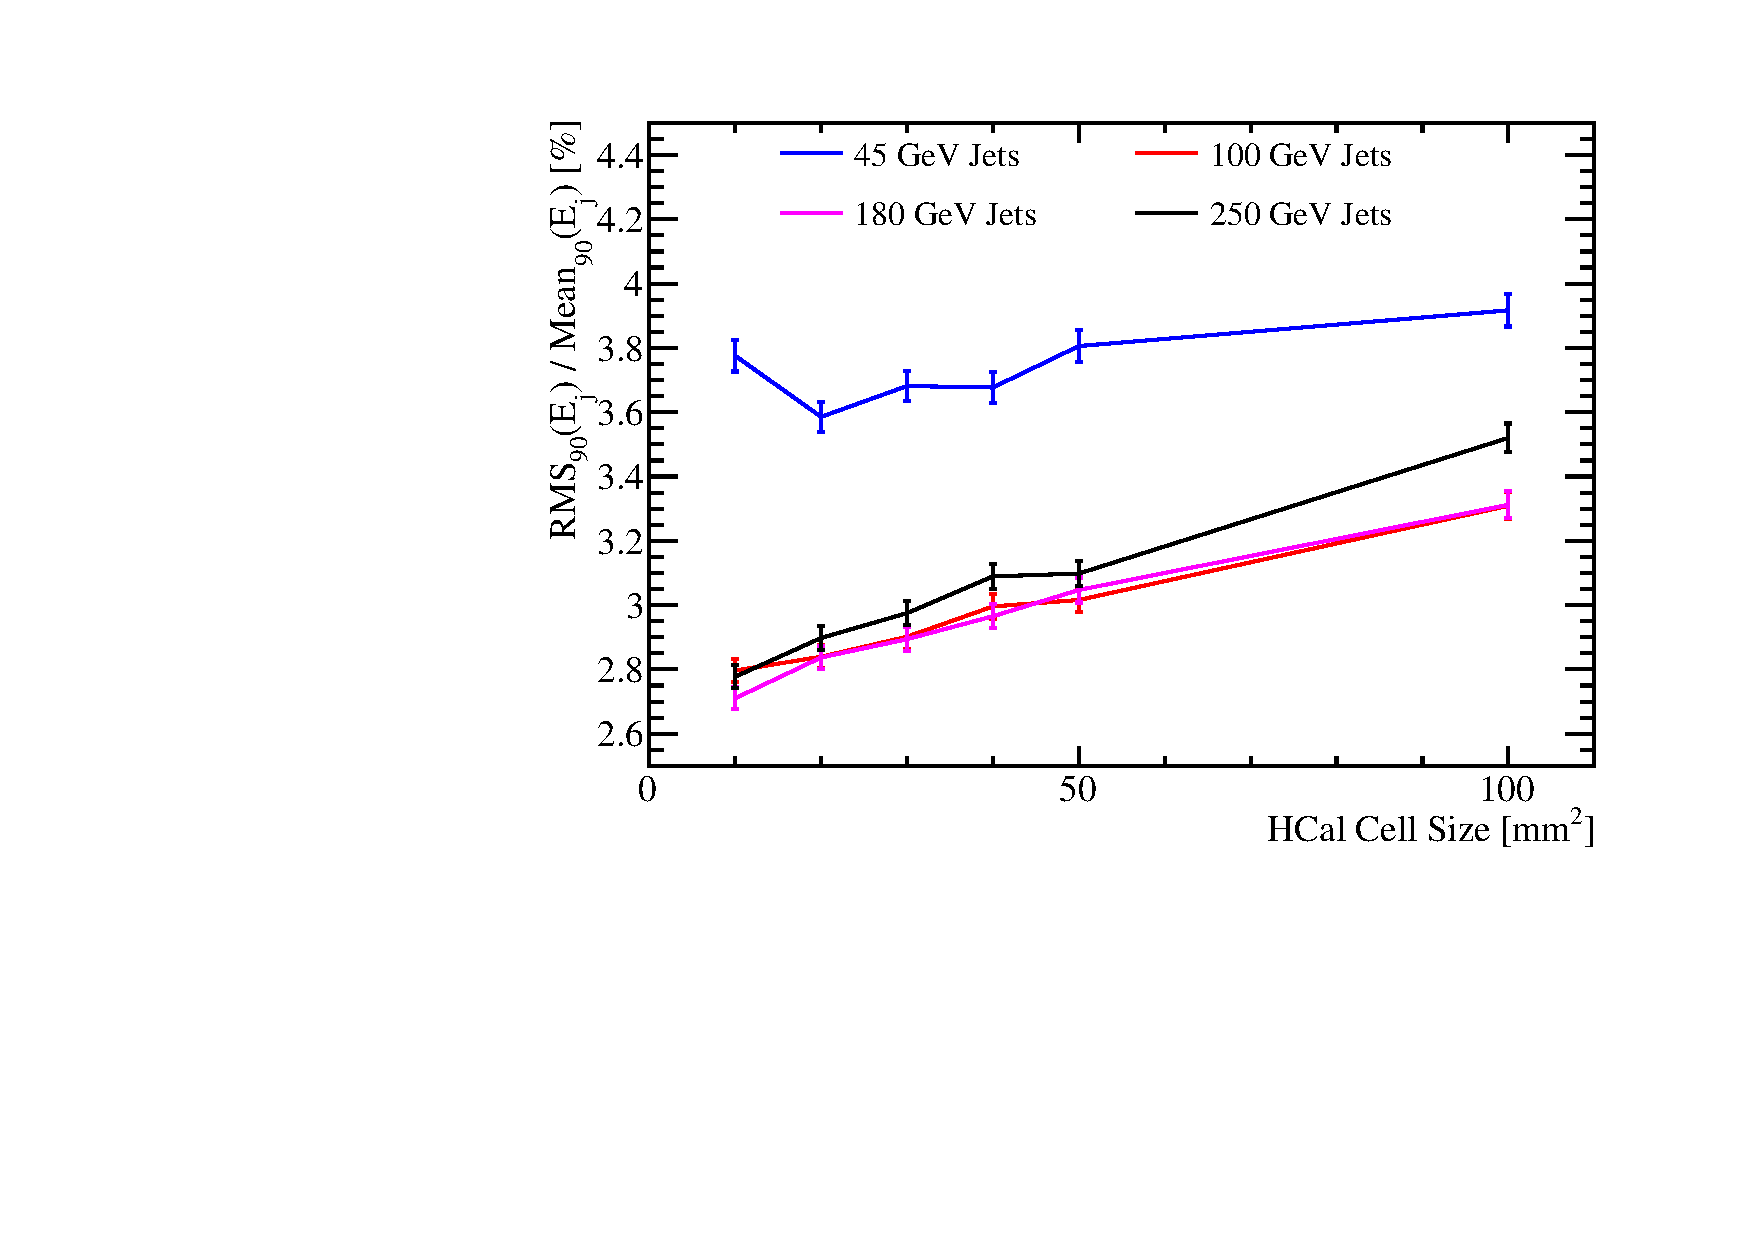
\includegraphics[width=0.5\textwidth]{OptimisationStudies/Plots/JetEnergyResolutions/JER_vs_HCalCellSize.pdf}
\caption[The jet energy resolution as a function of HCal cell size for various jet energies using the nominal ILD detector model.]{The jet energy resolution as a function of HCal cell size for various jet energies using the nominal ILD detector model.}
\label{fig:hcalcellsize}
\end{figure}

\begin{figure}[h!]
\centering
\subfloat[]{\label{fig:hcalcellsize45break}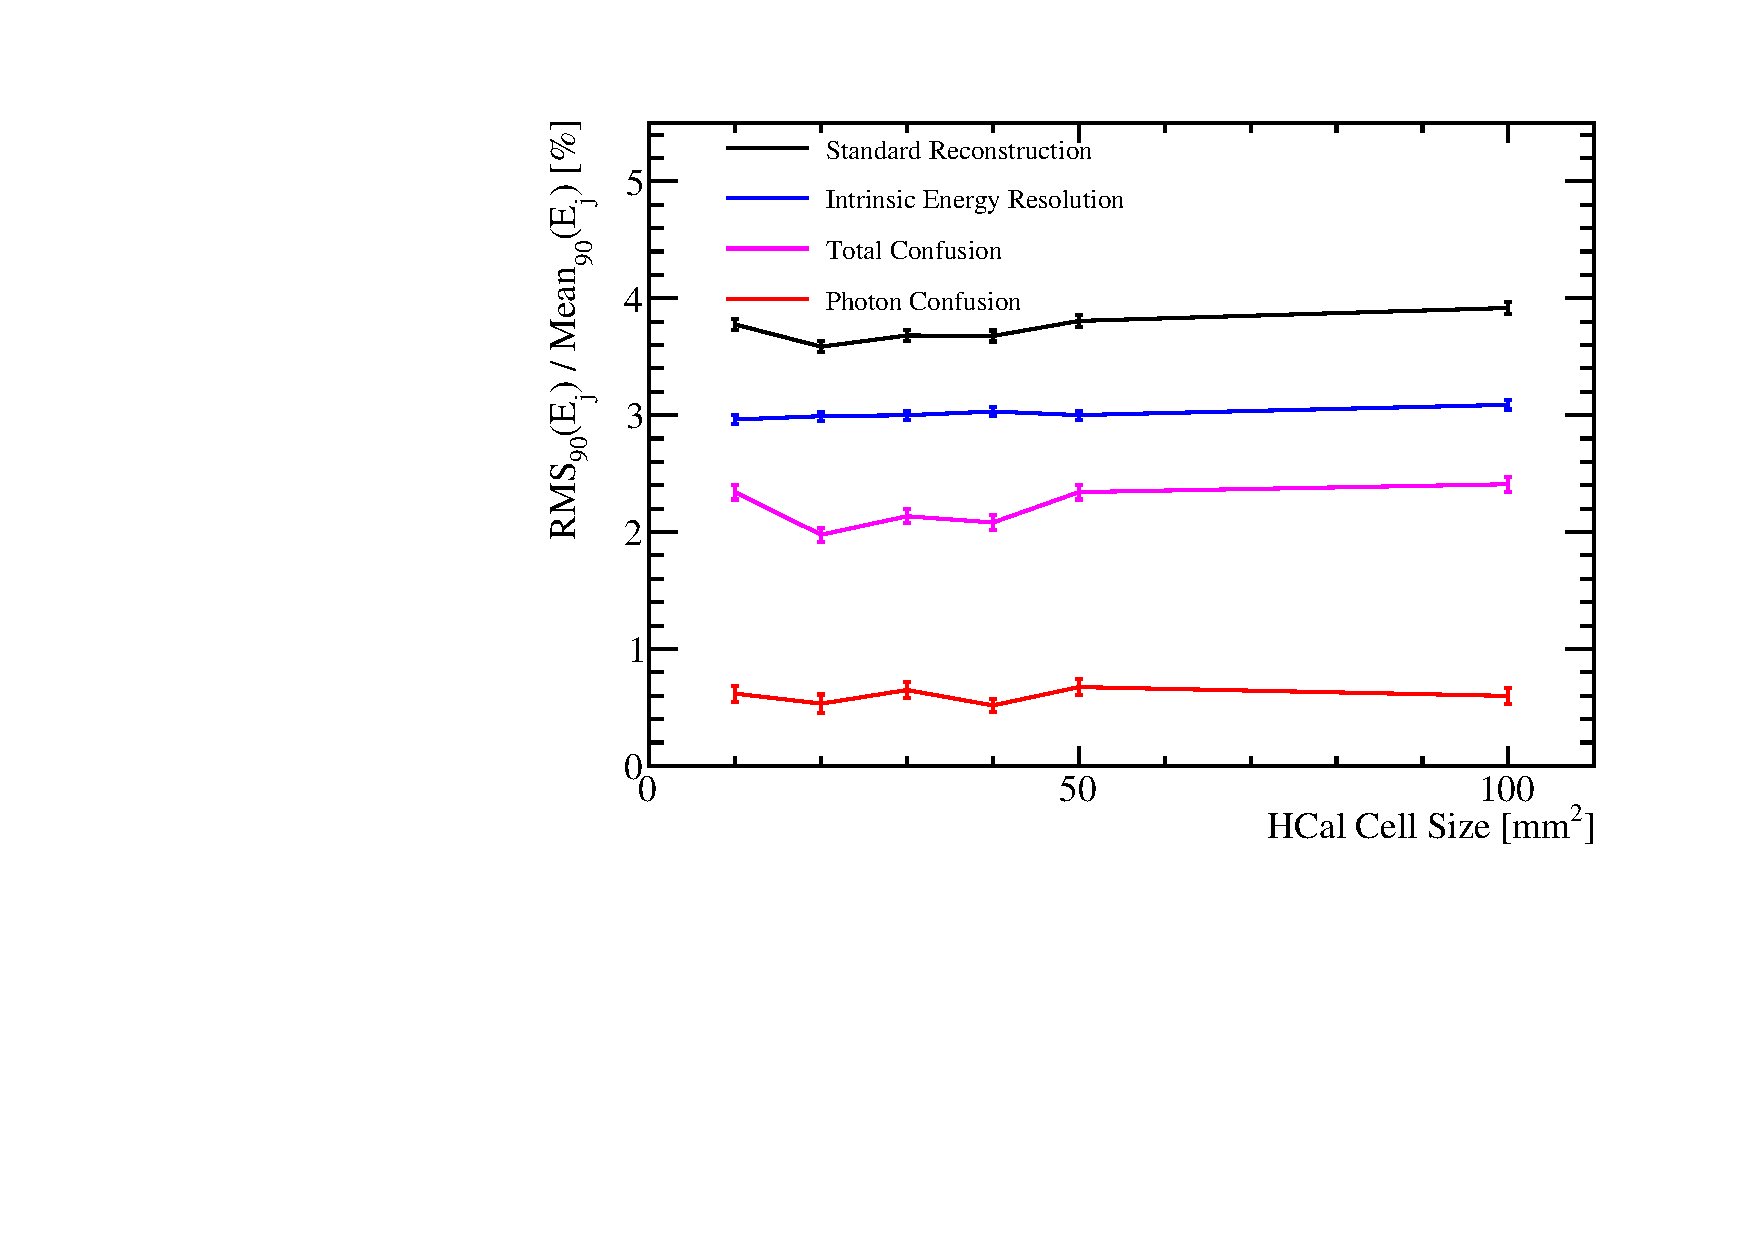
\includegraphics[width=0.5\textwidth]{OptimisationStudies/Plots/JetEnergyResolutions/JER_vs_HCalCellSize_91GeV_DiJet_Breakdown.pdf}}
\subfloat[]{\label{fig:hcalcellsize250break}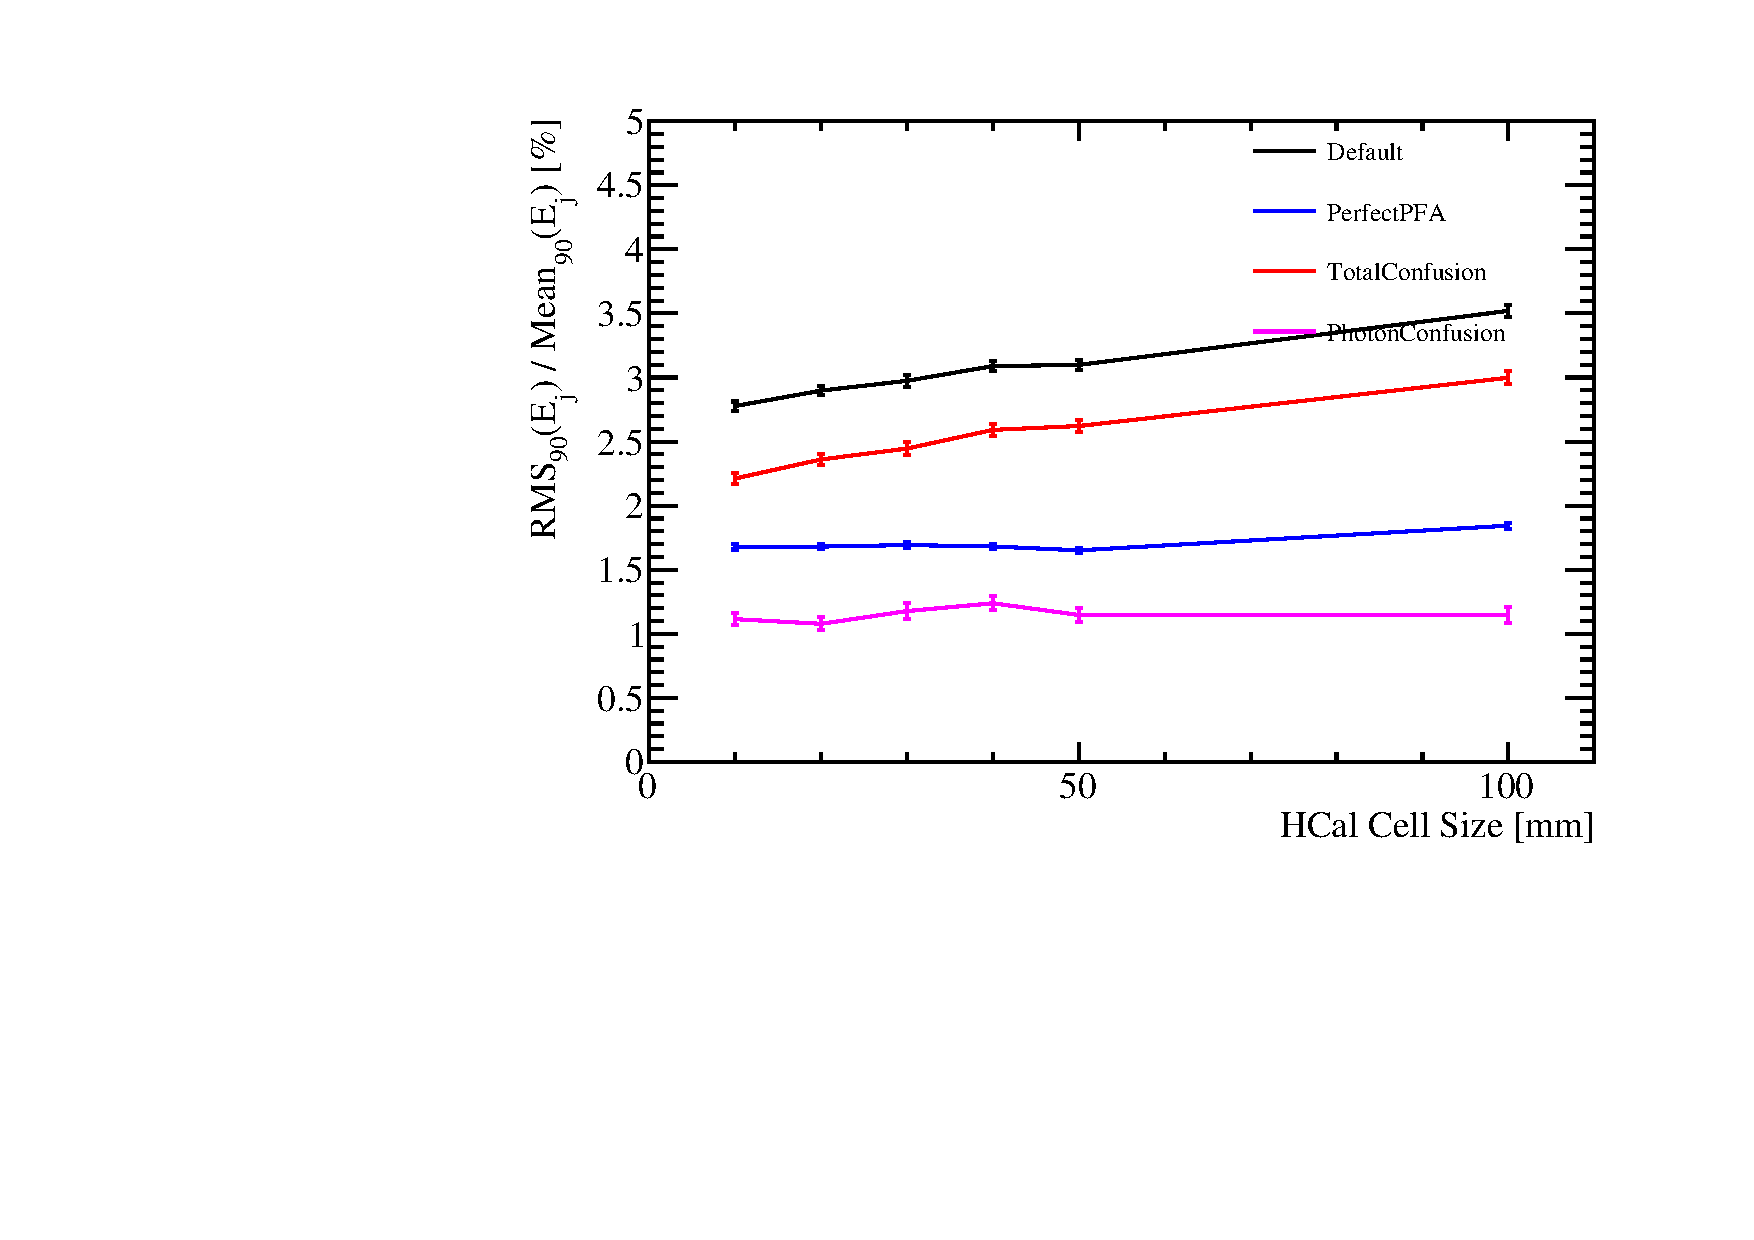
\includegraphics[width=0.5\textwidth]{OptimisationStudies/Plots/JetEnergyResolutions/JER_vs_HCalCellSize_500GeV_DiJet_Breakdown.pdf}}
\caption[Contributions to the jet energy resolution shown as function of HCal cell size using the nominal ILD detector model for \protect\subref{fig:hcalcellsize45break} 45~GeV jets and \protect\subref{fig:hcalcellsize250break} 250~GeV jets.  The black curves correspond to the standard reconstruction, the blue curves to the intrinsic energy resolution contribution to the jet energy resolution, the red curves to the confusion contribution to the jet energy resolution and the magenta curves to the confusion contribution to the jet energy resolution related solely to photon reconstruction.]{Contributions to the jet energy resolution shown as function of HCal cell size using the nominal ILD detector model for \protect\subref{fig:hcalcellsize45break} 45~GeV jets and \protect\subref{fig:hcalcellsize250break} 250~GeV jets.  The black curves correspond to the standard reconstruction, the blue curves to the intrinsic energy resolution contribution to the jet energy resolution, the red curves to the confusion contribution to the jet energy resolution and the magenta curves to the confusion contribution to the jet energy resolution related solely to photon reconstruction.}
\label{fig:hcalcellsizebreak}
\end{figure}

A comparison of the results from the ECal and HCal cell size optimisation studies shows that the jet energy resolution has a stronger dependency on the ECal cell size than on the HCal cell size; increasing the nominal ECal cell size by a factor of three makes the jet energy resolution for 250~GeV jets worse by $\sim 20\%$, while increasing the nominal HCal cell size by the same factor makes the jet energy resolution worse by $\sim 12\%$.  This is to be expected as in the particle flow paradigm $\approx 30\%$ of jet energy is recorded in the ECal, while only $\approx 10\%$ is recorded in the HCal.  Consequently, the potential effect of double counting and omitting energy deposits, i.e. confusion, is greater in the ECal than the HCal.  Therefore, minimising confusion in the ECal is expected to be more crucial for the overall jet energy resolution, which is what is observed.  Furthermore, as PandoraPFA groups calorimeter hits together using a cone clustering approach, identifying the start of a particle shower is key for determining how calorimeter hits are grouped together deeper into the calorimeters.  In effect, this means the grouping of calorimeter hits in the HCal depends upon information gathered in the ECal.  Therefore, if the ECal performance is sufficiently good, even with coarse HCal cell sizes, excellent performance can be achieved.  

In summary, the confusion contribution to the jet energy resolution falls as the HCal cell size is reduced, while the intrinsic energy resolution of the detector is largely unaffected.  As this dependancy is relatively weak, even the use of $100 \times 100 \text{ mm}^{2}$ HCal cell sizes would be enough to allow for separation of the hadronic decays of W and Z bosons, i.e. $\sigma_{E}/E \lesssim 3.8\%$ \cite{arXiv:0907.3577}, at ILC like energies.  However, there are benefits to having smaller HCal cell size; the jet energy resolution is reduced from $\sim3.5\%$ to $\sim2.8\%$ for 250~GeV jets when decreasing the HCal cell size from $100 \times 100 \text{ mm}^{2}$ to $10 \times 10 \text{ mm}^{2}$.  

%========================================================================================

\subsection{HCal Number of Layers}
\label{sec:hcalnlayers}
In this study, the total number of layers in the HCal was varied.  In contrast to the longitudinal sampling frequency study, the active and absorber layer thicknesses in the HCal were not altered.  Changing the number of layers in this way leads to a change in the total thickness of the calorimeter.  This study is sensitive to the effects, if any, of leakage of energy out of the back of the calorimeters.  The manufacturing cost of the HCal is proportional to the number of readout channels and layers.  Therefore, minimising the number of layers, while retaining excellent physics performance is important.  Here detector models were simulated with a HCal containing 36, 42, 48 (nominal), 54 and 60 layers. 

It is expected that the energy resolution of the detector will improve when the number of layers in the HCal is increased since fewer events should suffer from the effects of leakage.  Any improvements seen by increasing the number of layers in the HCal is expected only up to the point where the majority of hadronic showers are fully contained by the calorimeters.  The energy resolution as a function of number of layers in the HCal for 50~GeV $\text{K}^{0}_{L}$ is shown in figure \ref{fig:hcalnfixedlayerser}.  The energy resolution becomes worse as the number of layers in the HCal is reduced below 48 layers, while above this point additional layers do not change the energy resolution.  This indicates that the majority of hadronic showers at this energy are fully contained by a 48 layer HCal.  As reducing the number of HCal layers to 36 only causes a small degradation, $\sim 10\%$, in the neutral hadron energy resolution, it is feasible to consider reducing the number of layers in the ILD HCal.  

\begin{figure}[h!]
\centering
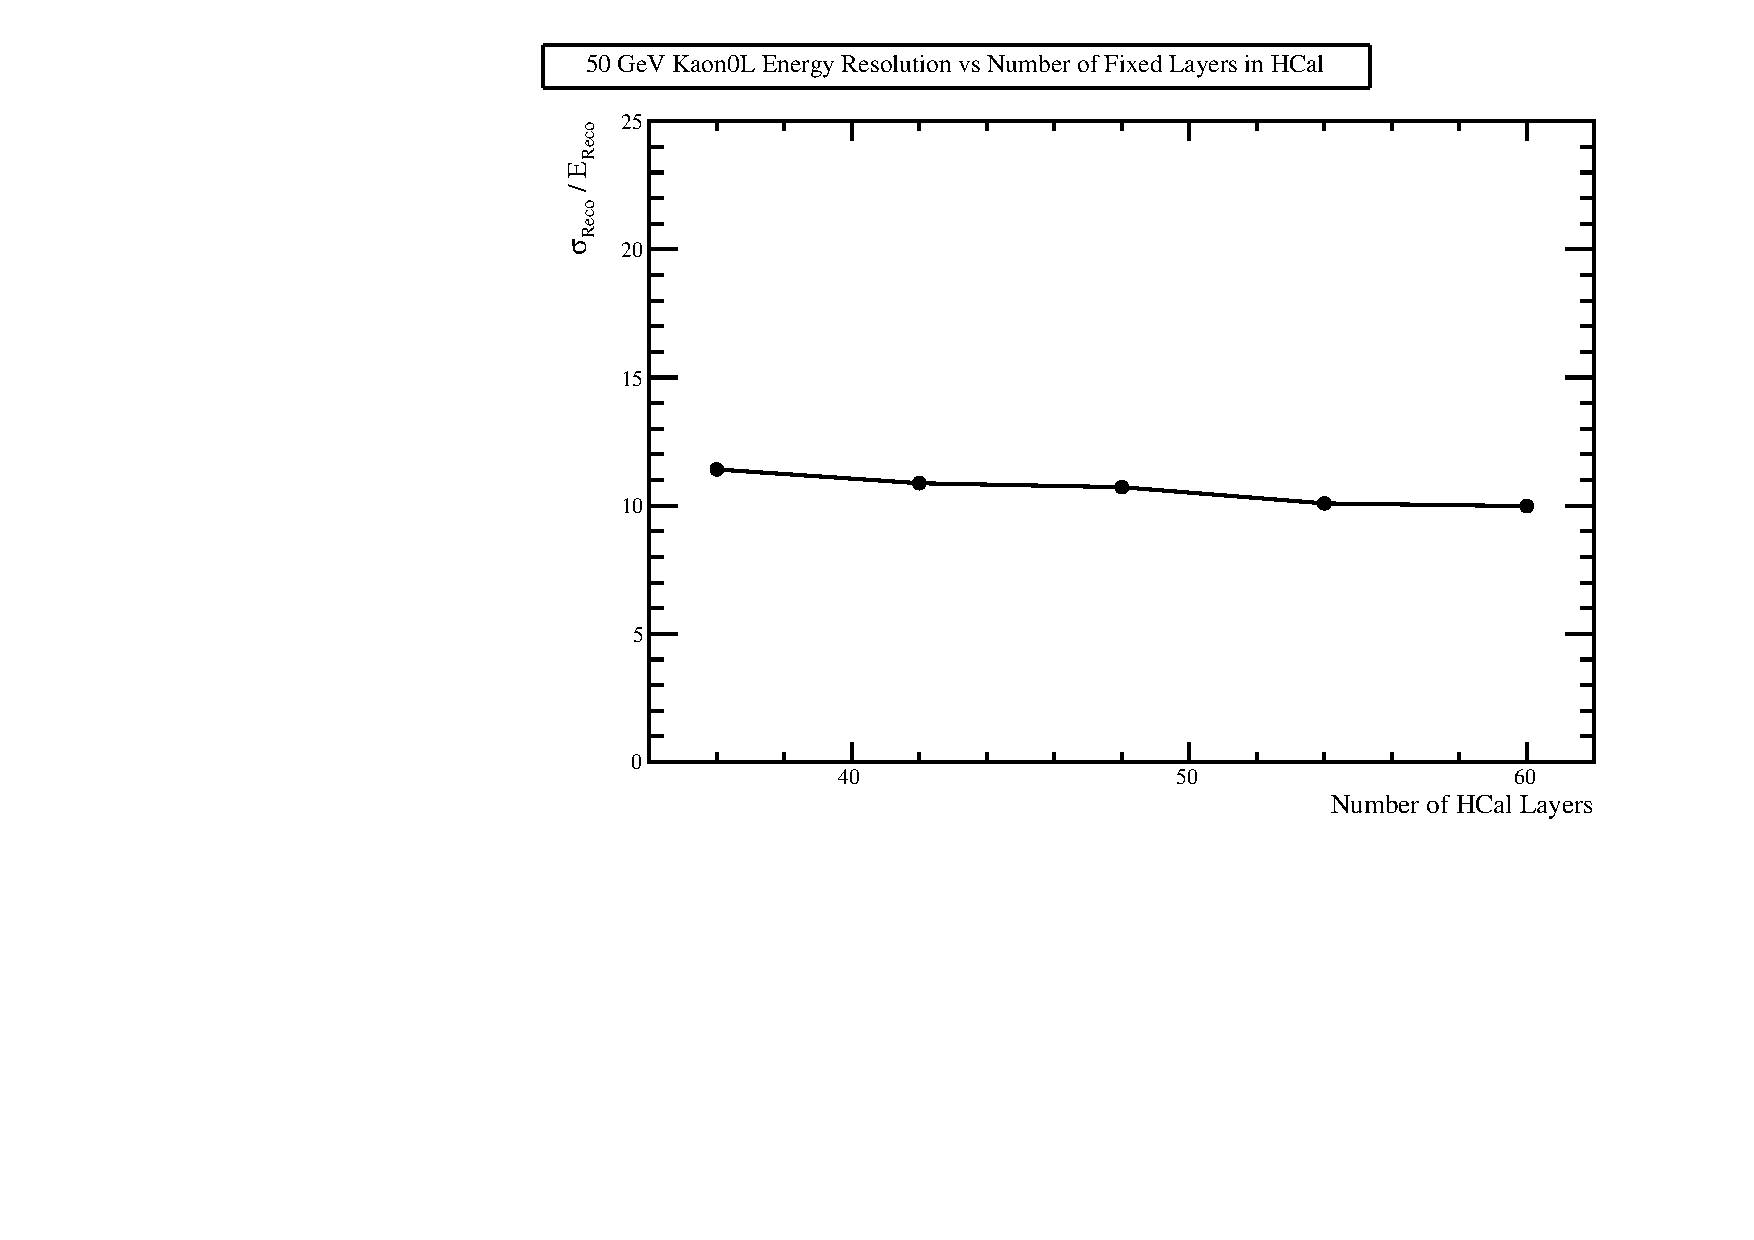
\includegraphics[width=0.5\textwidth]{OptimisationStudies/Plots/EnergyResolution/ER_vs_HCalNFixedLayers_50GeVKaon0L.pdf}
\caption[The energy resolution as a function of number of layers in the HCal for 50~GeV $\text{K}^{0}_{L}$ events using the nominal ILD detector model.]{The energy resolution as a function of number of layers in the HCal for 50~GeV $\text{K}^{0}_{L}$ events using the nominal ILD detector model.}
\label{fig:hcalnfixedlayerser}
\end{figure}

Figure \ref{fig:hcalnfixedlayers} shows the jet energy resolution as a function of the number of layers in the HCal.  For low energy jets, where intrinsic energy resolution dominates, the jet energy resolution does not depend on the number of layers in the HCal.  At high jet energies, where confusion dominates, increasing the number of layers in the HCal improves the jet energy resolution; the jet energy resolution is goes from $\sim3.4\%$ to $\sim3.0\%$ for 250~GeV jets when increasing the number of HCal layers from 36 to 48.  The origin of these trends is leakage of energy out of the back of the calorimeters, which becomes more problematic as the number of layers in the HCal is reduced and the jet energy increases.  

Figure \ref{fig:hcalnfixedlayersbreak} shows the jet energy resolution contributions as a function of the number of layers in the HCal.  These results appear somewhat counterintuitive in that the intrinsic energy resolution of the detector does not seem to depend on the number of layers in the HCal even for high energy jets.  However, this is expected given only 10\% of jet energy is carried in the form of neutral hadrons and the neutral hadron energy resolution, for 50~GeV hadrons, is only weakly dependent on the number of HCal layers.  Leakage does have an effect on the intrinsic energy resolution, however, the use of $\text{RMS}_{90}$ obscures part of this by excluding events where leakage is significant.  The fractional decrease in $\text{RMS}_{90}$ for the intrinsic energy distribution when increasing the number of HCal layers from 36 to 60 is $\sim4\%$, however, the change in the full RMS is $\sim23\%$.  Figure \ref{fig:hcalnfixedlayersbreak} also shows that the confusion contribution is far more sensitive to the number of layers in the HCal than the intrinsic energy resolution.  This sensitivity originates from the reclustering stage of the reconstruction in events where leakage has occurred.  In these events, when PandoraPFA compares the momentum of a charged particle track to the cluster of calorimeter hits that it produces, there will be a disparity.  To resolve the disparity, PandoraPFA will associate other calorimeter energy deposits that were not produced by the charged particle to the track to compensate for the leaked energy, which produces confusion.  As photons are largely contained within the ECal at these energies, the photon confusion contribution to the jet energy resolution has no dependence on the number of layers in the HCal. 

\begin{figure}[h!]
\centering
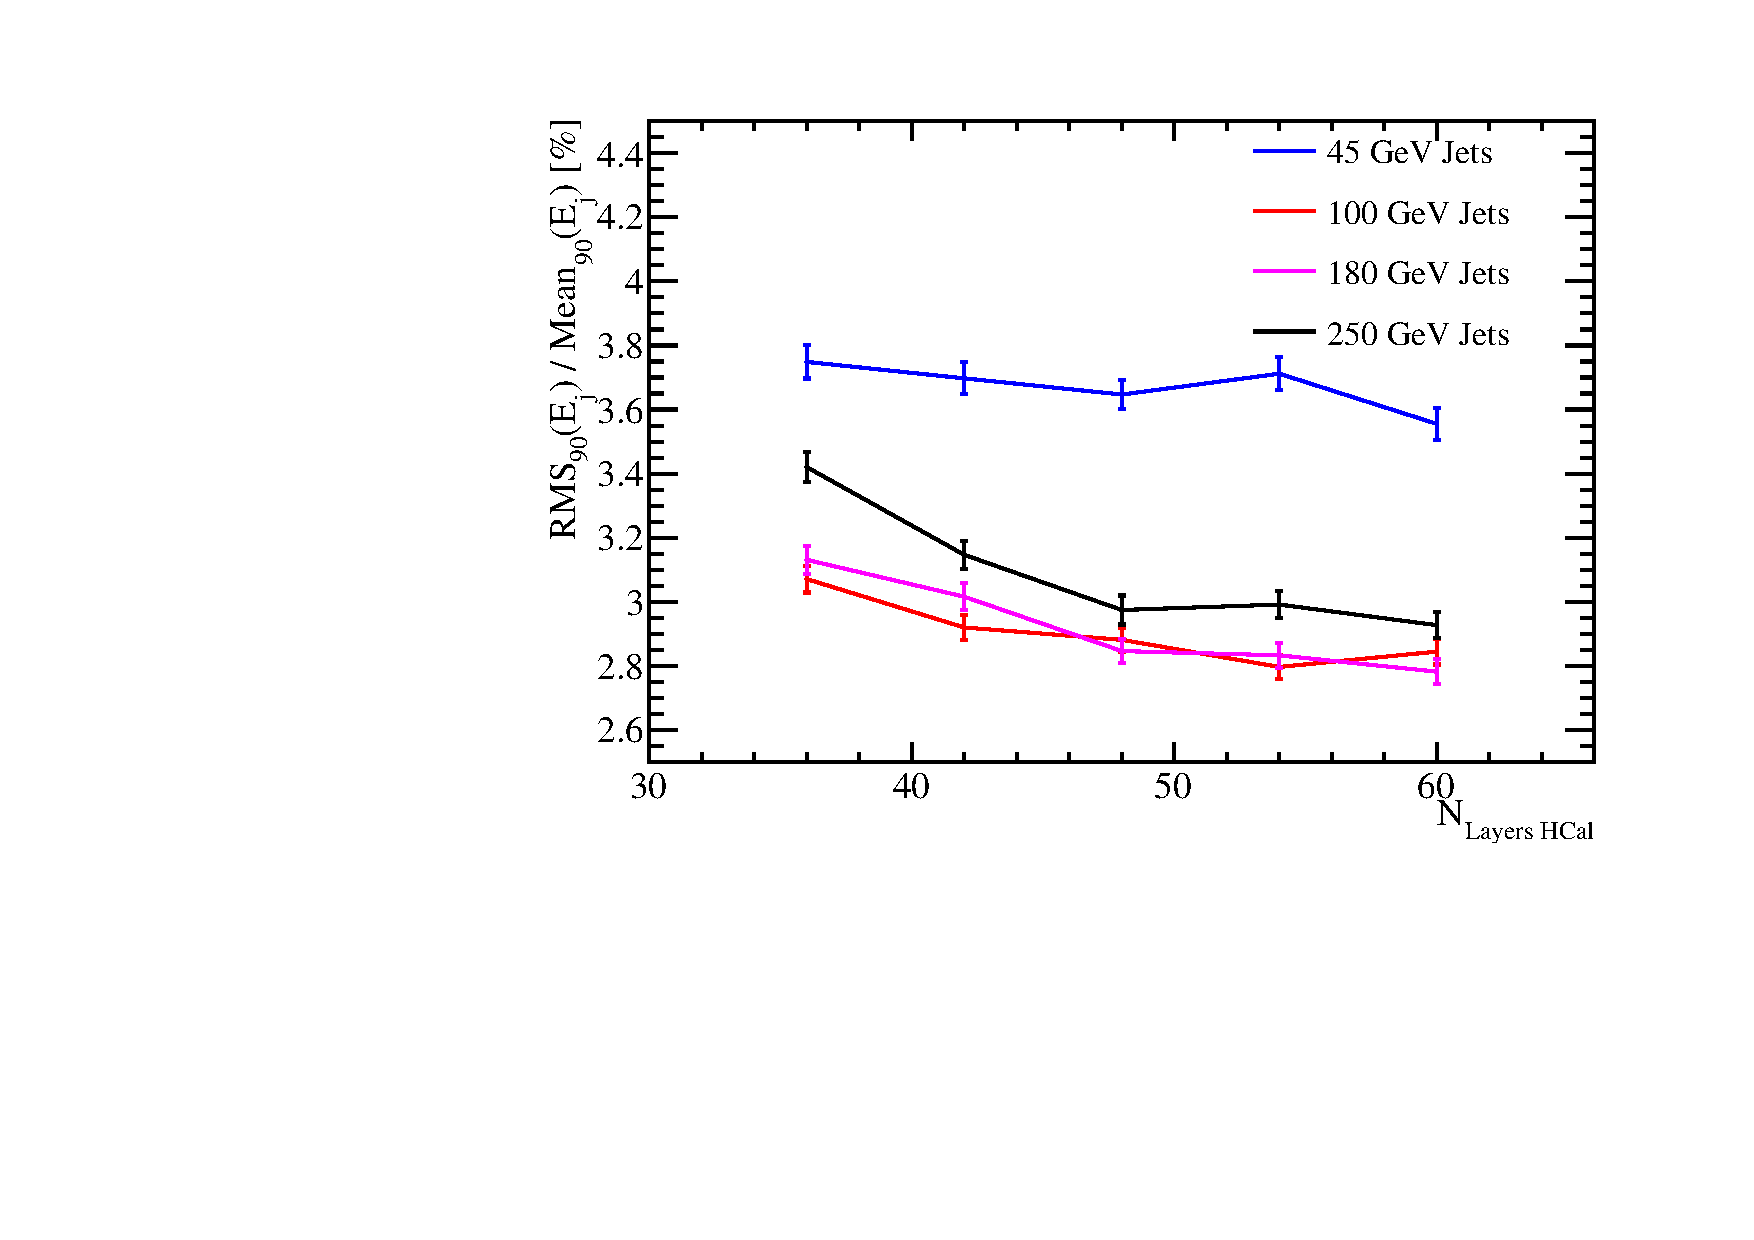
\includegraphics[width=0.5\textwidth]{OptimisationStudies/Plots/JetEnergyResolutions/JER_vs_NumberOfHCalLayersOfFixedDepth.pdf}
\caption[The jet energy resolution as a function of number of layers in the HCal for various jet energies using the nominal ILD detector model.]{The jet energy resolution as a function of number of layers in the HCal for various jet energies using the nominal ILD detector model.}
\label{fig:hcalnfixedlayers}
\end{figure}

\begin{figure}[h!]
\centering
\subfloat[]{\label{fig:hcalnfixedlayers45break}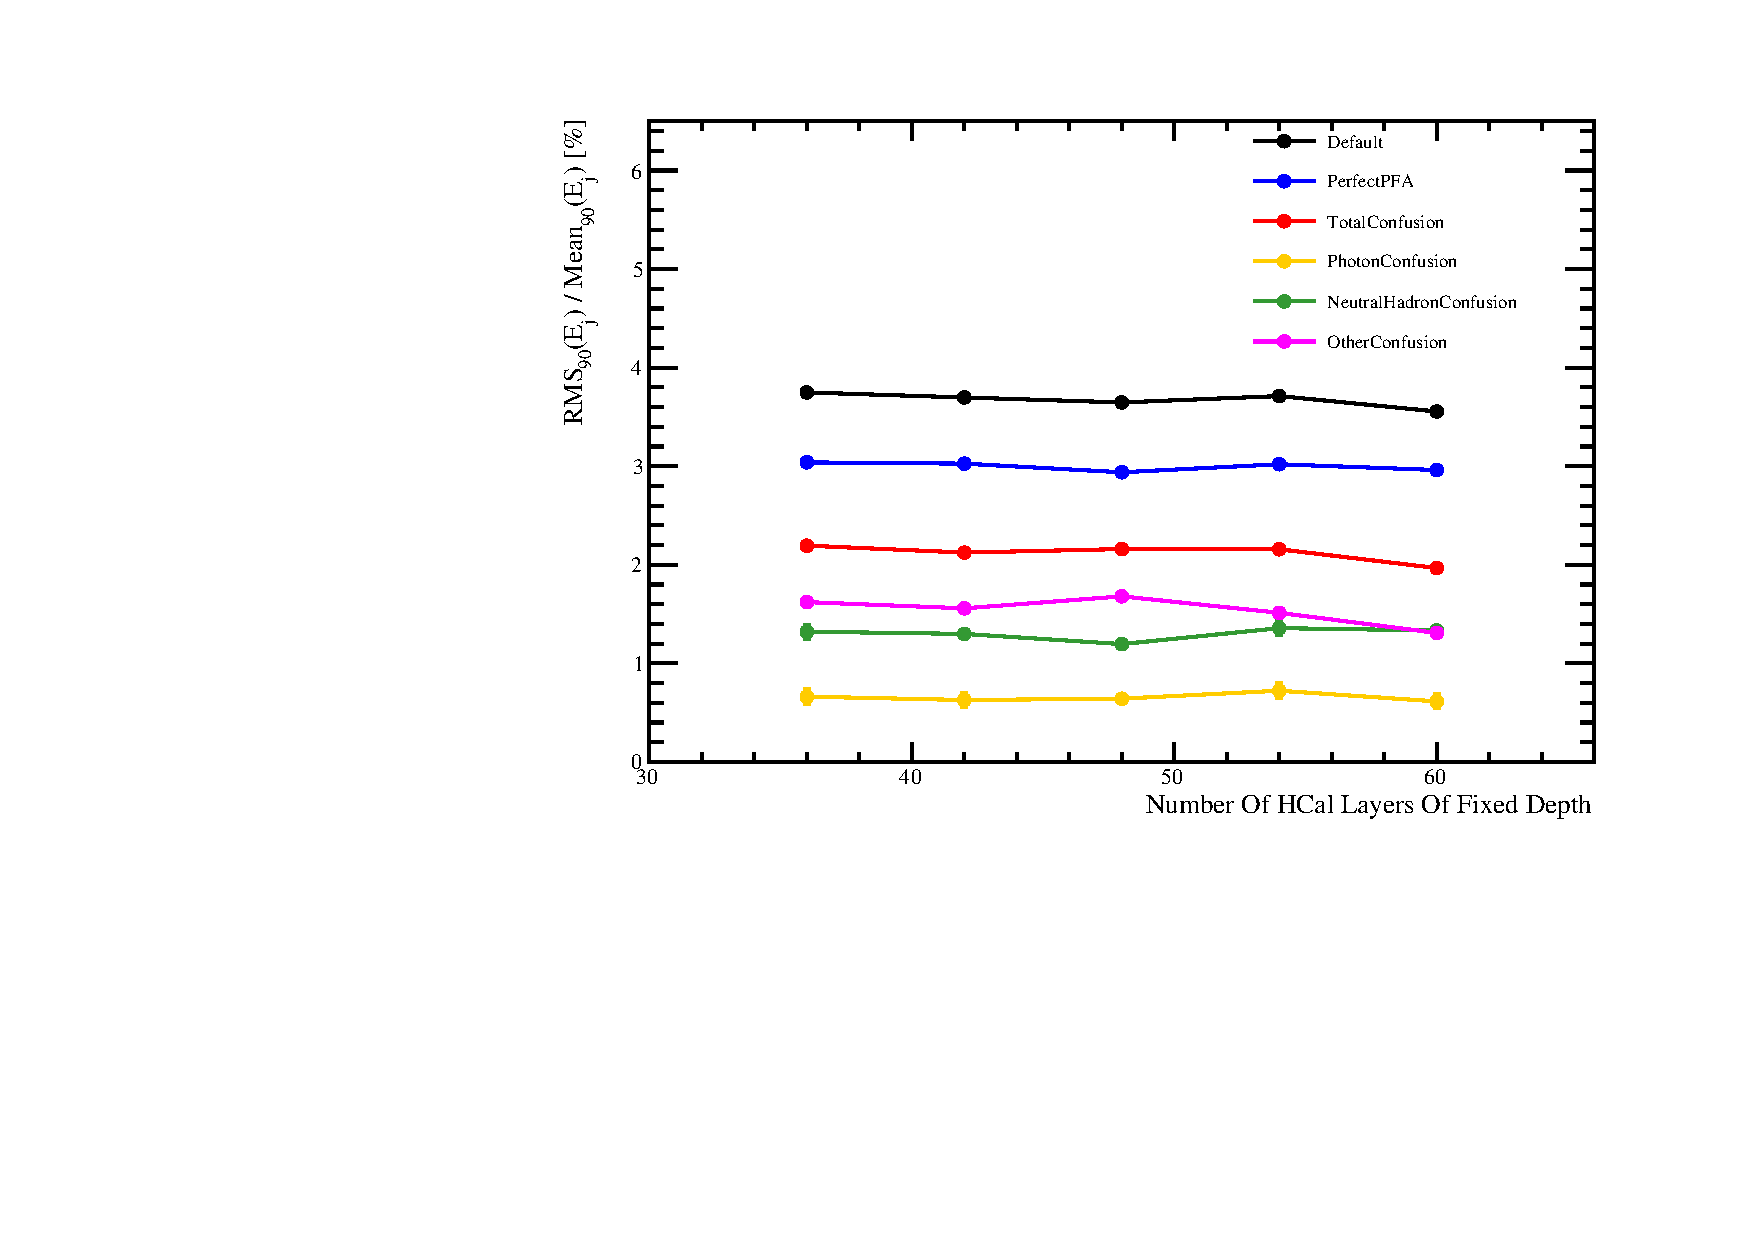
\includegraphics[width=0.5\textwidth]{OptimisationStudies/Plots/JetEnergyResolutions/JER_vs_NumberOfHCalLayersOfFixedDepth_91GeV_DiJet_Breakdown.pdf}}
\subfloat[]{\label{fig:hcalnfixedlayers250break}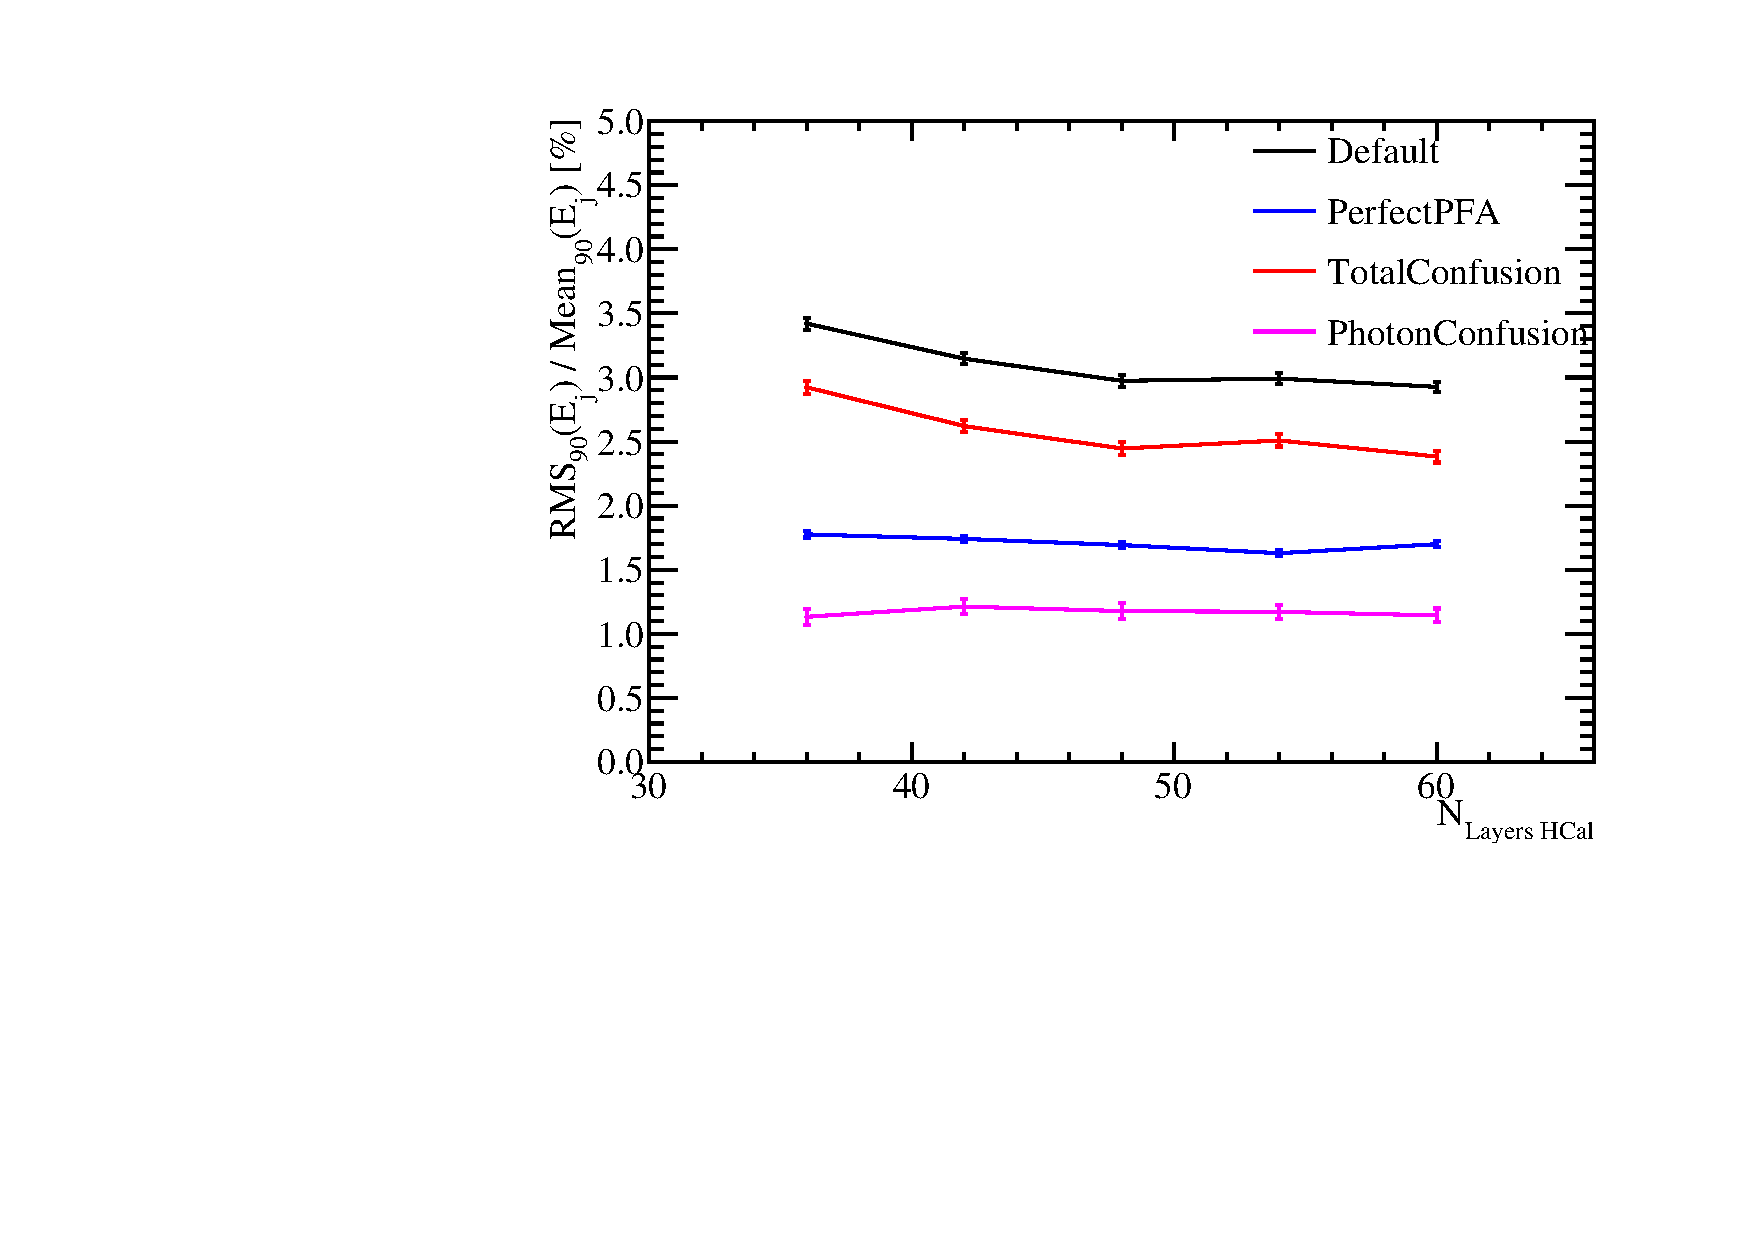
\includegraphics[width=0.5\textwidth]{OptimisationStudies/Plots/JetEnergyResolutions/JER_vs_NumberOfHCalLayersOfFixedDepth_500GeV_DiJet_Breakdown.pdf}}
\caption[Contributions to the jet energy resolution shown as function of number of layers in the HCal using the nominal ILD detector model for \protect\subref{fig:hcalnfixedlayers45break} 45~GeV jets and \protect\subref{fig:hcalnfixedlayers250break} 250~GeV jets.  The black curves correspond to the standard reconstruction, the blue curves to the intrinsic energy resolution contribution to the jet energy resolution, the red curves to the confusion contribution to the jet energy resolution and the magenta curves to the confusion contribution to the jet energy resolution related solely to photon reconstruction.]{Contributions to the jet energy resolution shown as function of number of layers in the HCal using the nominal ILD detector model for \protect\subref{fig:hcalnfixedlayers45break} 45~GeV jets and \protect\subref{fig:hcalnfixedlayers250break} 250~GeV jets.  The black curves correspond to the standard reconstruction, the blue curves to the intrinsic energy resolution contribution to the jet energy resolution, the red curves to the confusion contribution to the jet energy resolution and the magenta curves to the confusion contribution to the jet energy resolution related solely to photon reconstruction.}
\label{fig:hcalnfixedlayersbreak}
\end{figure}

In summary, even if the number of layers in the HCal were reduced by 25\%, the jet energy resolution would be sufficient for separating the hadronic decays of the W and Z bosons at ILC energies, i.e. $\sigma_{E}/E \lesssim 3.8\%$ \cite{arXiv:0907.3577}.  Although, the effects of leakage do make the jet energy resolution worse for ILC like energies, once the number of layers in the HCal is reduced from 48 layers, therefore, it is desirable to have a minimum of 48 layers in the ILD HCal.
  
%========================================================================================

\subsection{HCal Longitudinal Sampling Frequency}
\label{sec:hcalsamplingfrequency}
Several detector models were simulated where the longitudinal sampling frequency in the HCal was modified.  The longitudinal sampling frequency was altered by changing the number of layers in the HCal, while simultaneously changing the active and absorber layer thicknesses, to maintain the total number of nuclear interaction lengths.  For each model considered, the absorber material was steel, containing a total of 5.72~$\lambda_{I}$, and the active material was scintillator, containing a total of 0.19~$\lambda_{I}$.  The ratio of the active to absorber layers thicknesses (the sampling fraction) in these models is the same as in the nominal ILD HCal.  A summary of the detector models considered is given in table \ref{table:nlayershcaloption}.  

\begin{table}[h!]
\centering
\begin{tabular}{ l l l }
\hline
Number $N_{\text{Layers HCal}}$ & Absorber Thickness & Active Thickness \\
 & [mm] & [mm] \\
\hline
60 & 16.00 & 2.40 \\ 
54 & 17.78 & 2.67 \\
48 & 20.00 & 3.00 \\
42 & 22.86 & 3.43 \\
36 & 26.67 & 4.00 \\
30 & 32.00 & 4.80 \\
24 & 40.00 & 6.00 \\
18 & 53.33 & 8.00 \\
\hline
\end{tabular}
\caption[Longitudinal configuration of the HCal in the detector models considered.]{Longitudinal configuration of the HCal in the detector models considered.}
\label{table:nlayershcaloption}
\end{table}

Figure \ref{fig:hcalnlayerser} shows the energy resolution for 50~GeV $\text{K}^{0}_{L}$ as a function of number of layers in the HCal.  As the number of layers in the HCal is increased, the energy resolution improves.  This is because increasing the number of layers in a sampling calorimeter, while leaving the total material budget unchanged, will lead to greater sampling of particles showering within it and a reduction the stochastic contribution to the energy resolution.  The energy resolution is less pronounced than the naive expectation of 1/$N_{\text{HCal}}$, where $N_{\text{HCal}}$ is the number of layers in the HCal, because this relationship only holds for the energy resolution of a single sampling calorimeter and these results are for the full ILD detector, including the $\approx 1 \lambda_{I}$ in the ECal.  Furthermore, the 1/$N_{\text{HCal}}$ functional form neglects a number of effects, such as instrumentation defects and electrical noise, that should be included when parameterising the energy resolution \cite{Fabjan:2003aq}.  

\begin{figure}[h!]
\centering
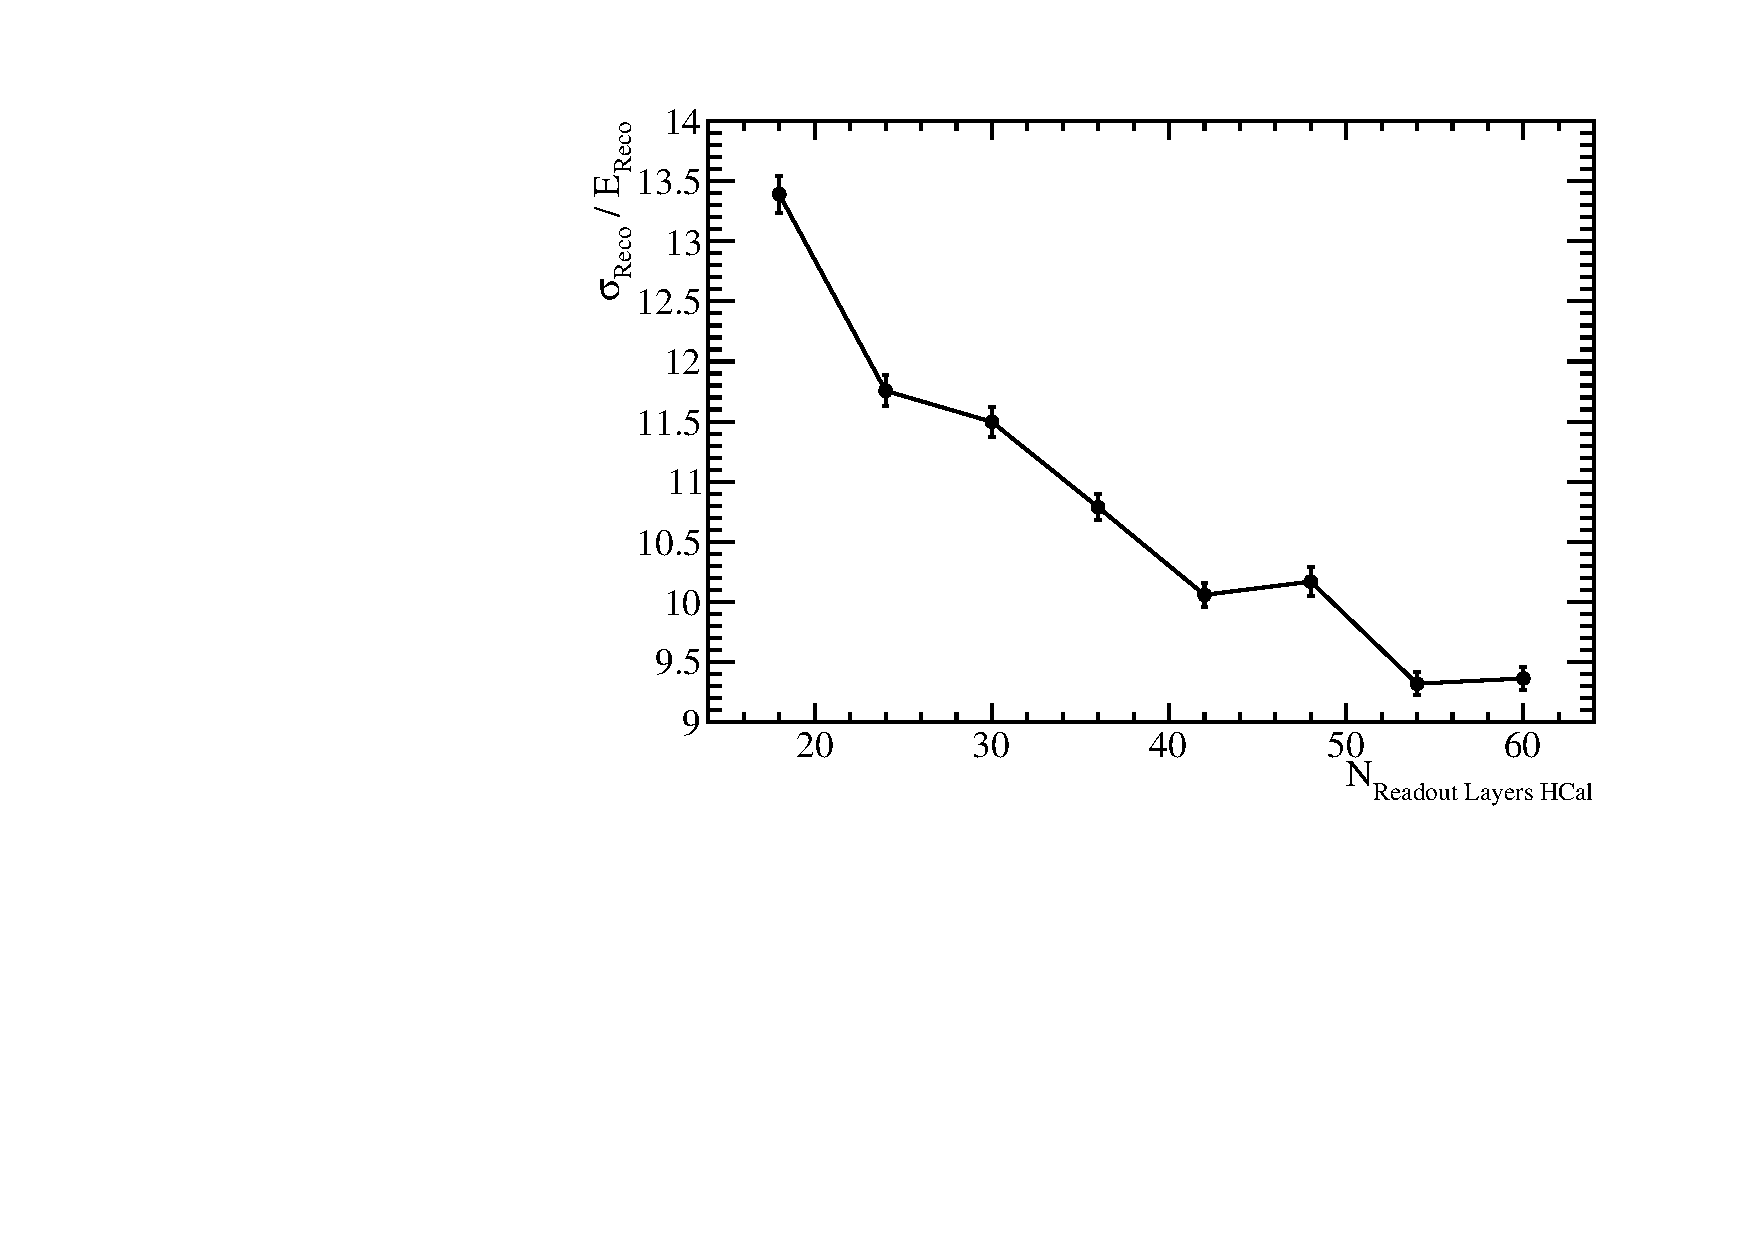
\includegraphics[width=0.5\textwidth]{OptimisationStudies/Plots/EnergyResolution/ER_vs_NHCalVariableLayers_50GeVKaon0L.pdf}
\caption[The energy resolution as a function of the longitudinal sampling frequency in the HCal for 50~GeV $\text{K}^{0}_{L}$ events using the nominal ILD detector model.]{The energy resolution as a function of the longitudinal sampling frequency in the HCal for 50~GeV $\text{K}^{0}_{L}$ events using the nominal ILD detector model.}
\label{fig:hcalnlayerser}
\end{figure}  

Figure \ref{fig:hcalnlayers} shows the jet energy resolution as a function of the longitudinal sampling frequency in the HCal.  Increasing the number of layers in the HCal leads to an improvement in the HCal; when the number of layers in the HCal is increased from 18 to 60 the jet energy resolution for 250~GeV jets improves by $\sim17\%$.  

Figure \ref{fig:hcalnlayersbreak} shows that both the intrinsic energy resolution and confusion improve with increasing longitudinal sampling frequency.  For 250~GeV jets, when increasing the number of HCal layers from 18 to 60 the intrinsic energy resolution contribution goes from $\sim 1.9\%$ to $\sim 1.6\%$ and the confusion contribution goes from $\sim 3.0\%$ to $\sim 2.4\%$.  The twofold improvement is expected because increasing the longitudinal sampling frequency improves the intrinsic energy resolution of a sampling calorimeter, which has the knock-on effect of lowering the confusion.  The resulting reduction in confusion is due to the improved precision obtained when comparing the momenta of charged particle tracks and the energy of clusters of calorimeter hits.  These comparisons are used to guide event reconstruction in PandoraPFA, therefore, if the precision of these comparisons is improved, the confusion is reduced as described in section \ref{sec:jerdecomposition}.   

\begin{figure}[h!]
\centering
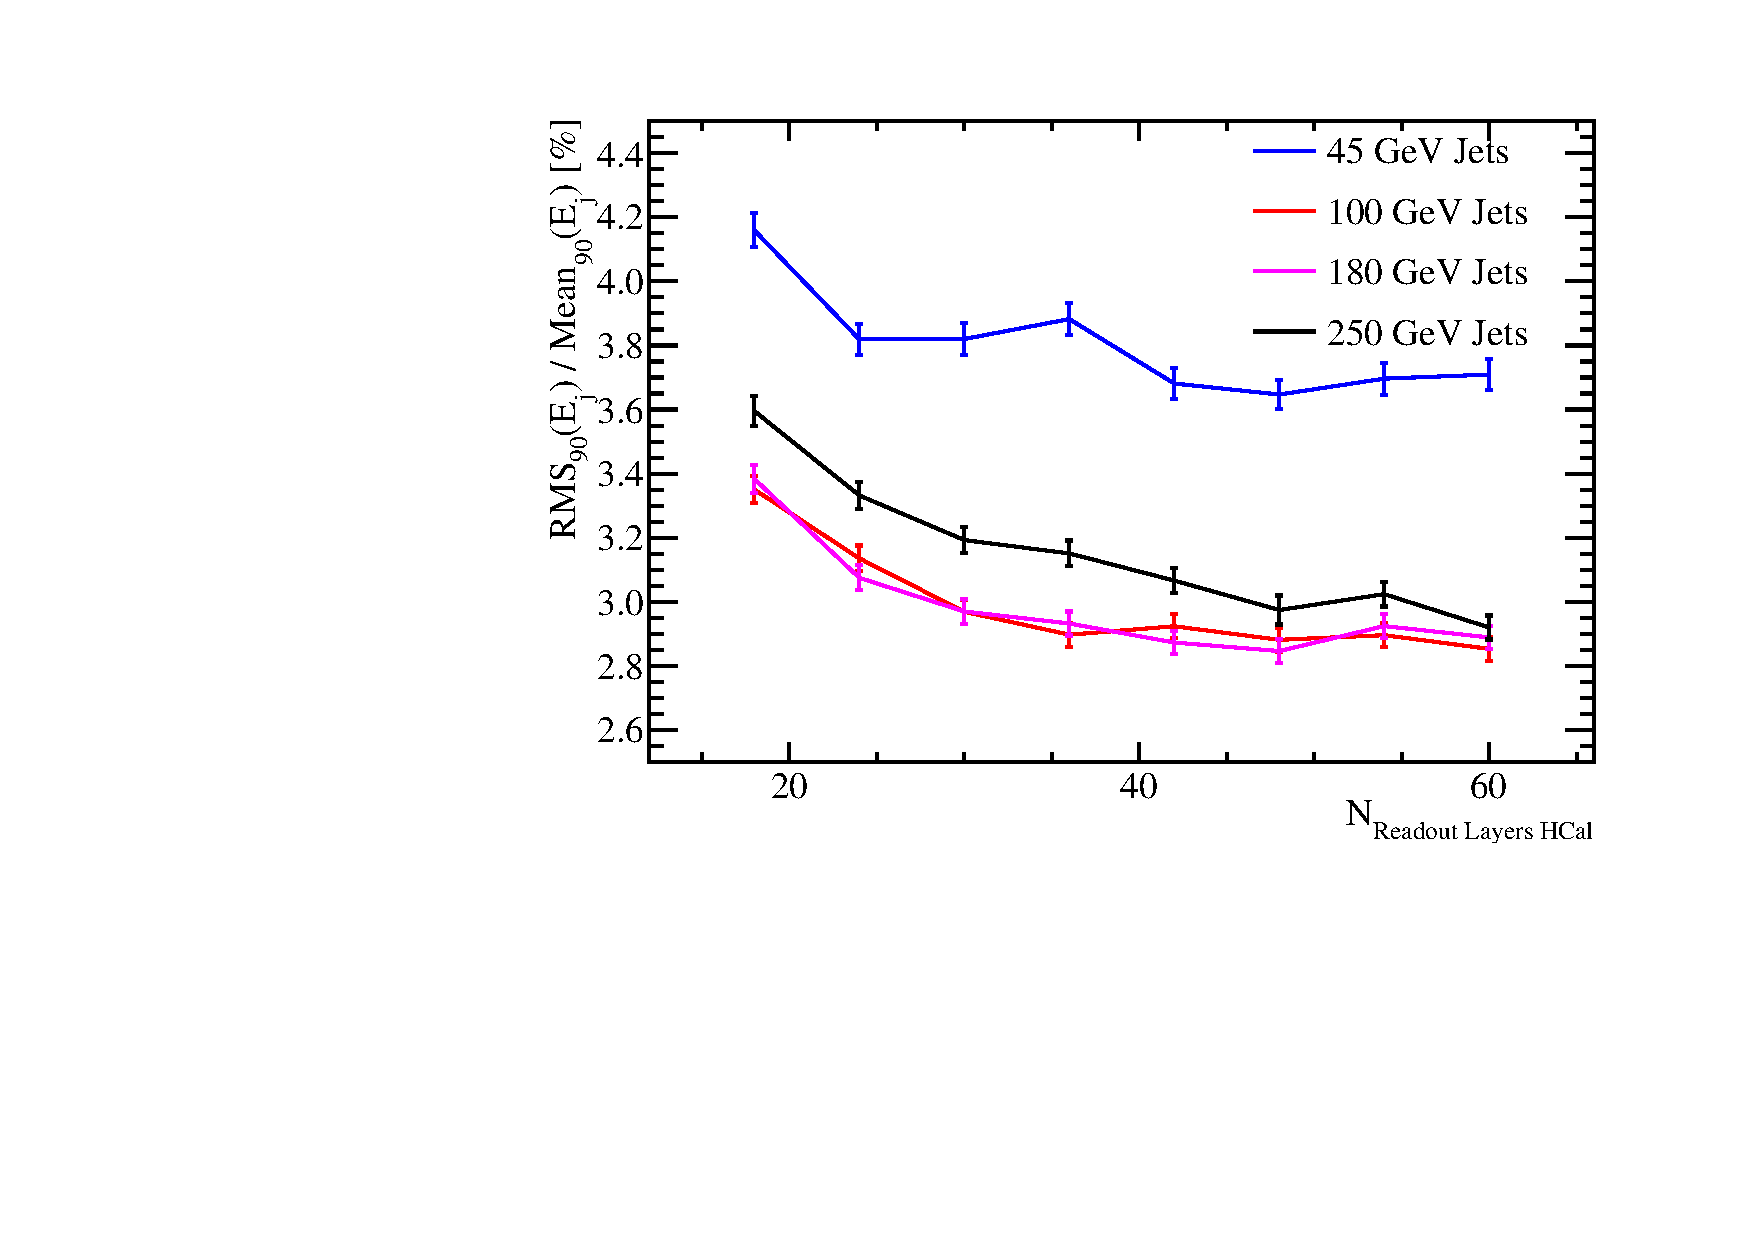
\includegraphics[width=0.5\textwidth]{OptimisationStudies/Plots/JetEnergyResolutions/JER_vs_NumberOfLayersInTheHCal.pdf}
\caption[The jet energy resolution as a function of longitudinal sampling frequency in the HCal for various jet energies using the nominal ILD detector model.]{The jet energy resolution as a function of longitudinal sampling frequency in the HCal for various jet energies using the nominal ILD detector model.}
\label{fig:hcalnlayers}
\end{figure}

\begin{figure}[h!]
\centering
\subfloat[]{\label{fig:hcalnlayers45break}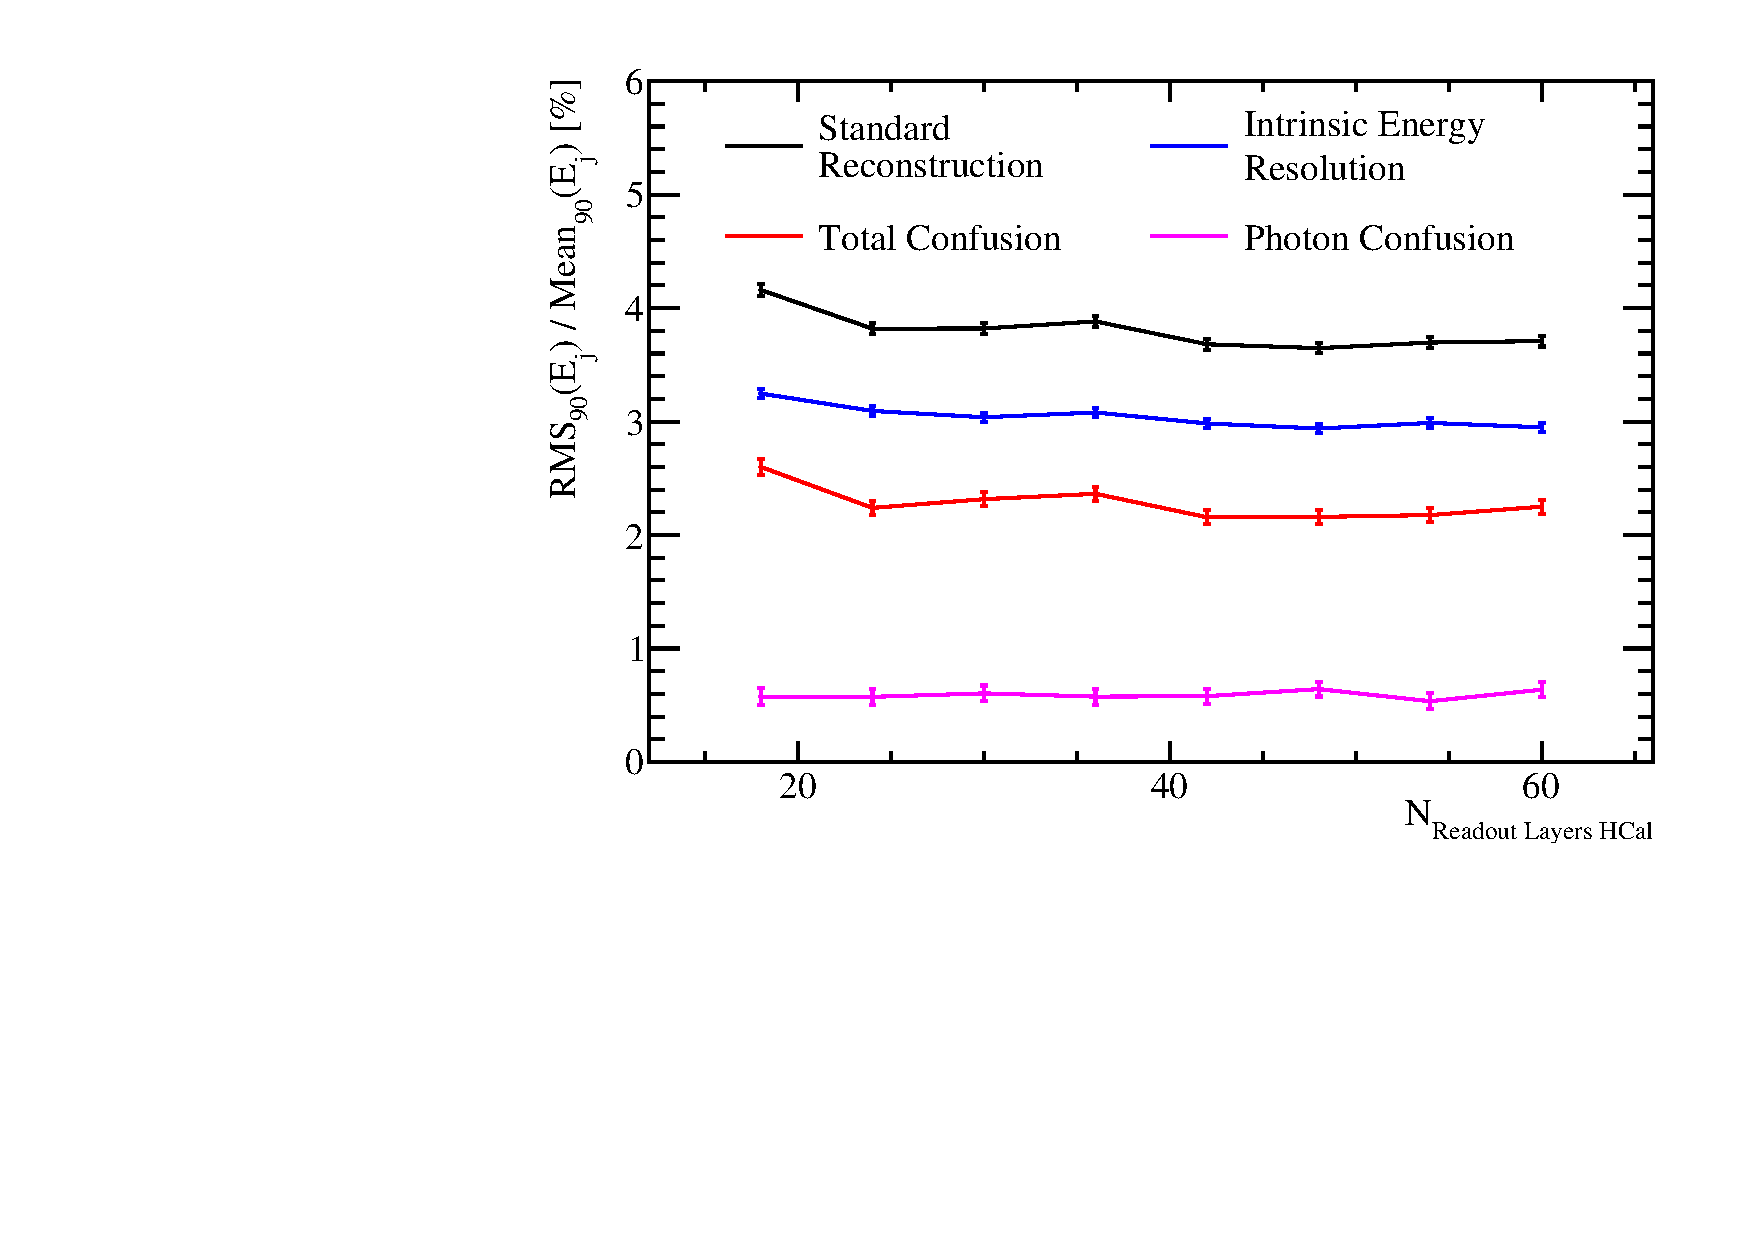
\includegraphics[width=0.5\textwidth]{OptimisationStudies/Plots/JetEnergyResolutions/JER_vs_NumberOfLayersInTheHCal_91GeV_DiJet_Breakdown.pdf}}
\subfloat[]{\label{fig:hcalnlayers250break}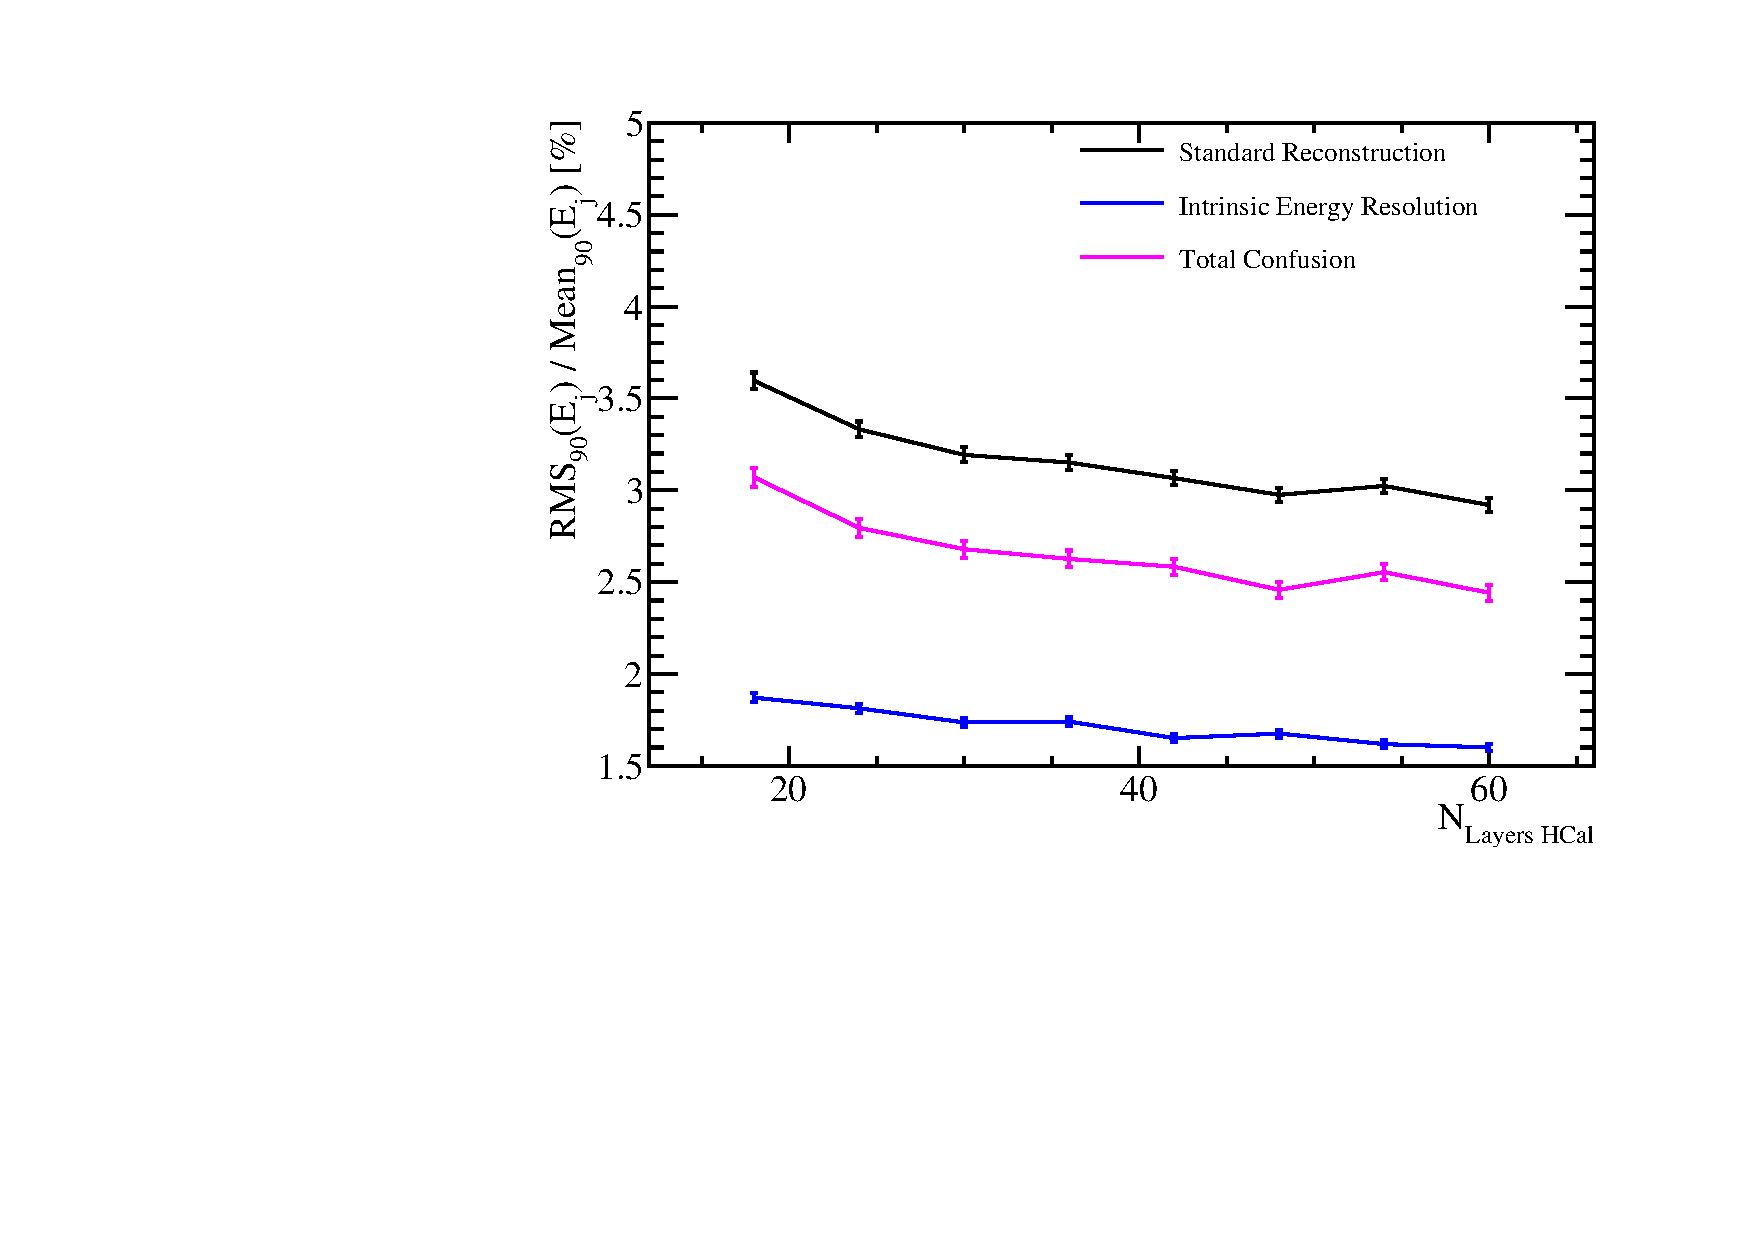
\includegraphics[width=0.5\textwidth]{OptimisationStudies/Plots/JetEnergyResolutions/JER_vs_NumberOfLayersInTheHCal_500GeV_DiJet_Breakdown.pdf}}
\caption[Contributions to the jet energy resolution shown as function of the longitudinal sampling frequency in the HCal using the nominal ILD detector model for \protect\subref{fig:hcalnlayers45break} 45~GeV jets and \protect\subref{fig:hcalnlayers250break} 250~GeV jets.  The black curves correspond to the standard reconstruction, the blue curves to the intrinsic energy resolution contribution to the jet energy resolution, the red curves to the confusion contribution to the jet energy resolution and the magenta curves to the confusion contribution to the jet energy resolution related solely to photon reconstruction.]{Contributions to the jet energy resolution shown as function of the longitudinal sampling frequency in the HCal using the nominal ILD detector model for \protect\subref{fig:hcalnlayers45break} 45~GeV jets and \protect\subref{fig:hcalnlayers250break} 250~GeV jets.  The black curves correspond to the standard reconstruction, the blue curves to the intrinsic energy resolution contribution to the jet energy resolution, the red curves to the confusion contribution to the jet energy resolution and the magenta curves to the confusion contribution to the jet energy resolution related solely to photon reconstruction.}
\label{fig:hcalnlayersbreak}
\end{figure}

It is clear that a larger number of layers in the HCal benefits both the intrinsic energy resolution of the ILD detector as well as reducing the confusion contribution to the jet energy resolution.  As there are few physics analyses that rely on the identification and categorisation of individual neutral hadrons, but there are many that rely on identification and categorisation of photons, the intrinsic energy resolution of the HCal is less crucial from a physics perspective than that of the ECal.  However, these studies show the HCal has a crucial role to play in jet reconstruction in the particle flow paradigm.  To achieve a jet energy resolution of $\sigma_{E}/E \lesssim 3.8\%$ \cite{arXiv:0907.3577}, which is required to separate the W and Z hadronic decays, the ILD detector will require a minimum of 42 layers in the HCal.  This longitudinal sampling frequency is required particularly for low energy jets where the energy resolution is dominated by the intrinsic energy resolution of the detector.

%========================================================================================

\subsection{HCal Sampling Fraction}
\label{sec:hcalsamplingfraction}
The performance of the ILD detector was studied for different ratios of active to absorber \textcolor{blue}{layer} thicknesses in the HCal.  In the nominal detector model, the active scintillator layer thickness is 3~mm, while the absorber layer thickness is 20~mm giving a sampling fraction of 0.15.  HCal models were simulated where this ratio was changed from 0.05 to 0.25 in steps of 0.05, while retaining the same number of interaction lengths.  

No performance changes in the energy resolution for 50~GeV $\text{K}^{0}_{L}$s or the jet energy resolution for 91, 200, 360 and 500~GeV Z$\rightarrow$uds di-jet events were observed when varying the ratio of active to absorber later thicknesses.  Based on these simulations, there is no suggestion that varying this ratio has any statistically significant effect on the physics performance.  Although this study indicates that thinning the active layer thickness would not change performance, hardware effects must also be considered to determine whether these conclusions hold true in a real detector.  A study into the effects of the readout electronics is required before changing the active layer thicknesses to determine whether a MIP signal can be clearly distinguished when changing the sampling fraction.  

%========================================================================================

\subsection{HCal Absorber Material}
\label{sec:hcalabsorbermaterial}
The nominal choice of HCal absorber material is steel with tungsten providing a feasible alternative \cite{Blaising:2015nla}.  Although tungsten is more expensive than steel, it contains a larger number of nuclear interaction lengths per unit length.  Therefore, using tungsten as the absorber material would allow for a reduction in the size of the HCal, while retaining the same number of nuclear interaction lengths.  Reducing the depth of the calorimeter would decrease the size of the solenoid required, which would offset some of the additional cost of tungsten. 

Table \ref{table:hcalabsmaterial} shows the configuration for the steel and tungsten HCal options that were used in the full ILD simulation.  To isolate the effects of changing the absorber material, the total depth, in nuclear interaction lengths, was kept constant when comparing the two options.  Furthermore, the sampling fraction was also held constant.  A number of different physics lists exist within GEANT4 for the modelling of hadronic showers.  The default model for high energy physics calorimetry is the QGSP\_BERT physics list.  This uses the quark-gluon string model \cite{Folger:2003sb} with the precompound model of nuclear evaporation \cite{geantStringModel} (QGSP) for high energy interactions and the Bertini (BERT) cascade model \cite{Guthrie:1968ue} for intermediate energy interactions.  For the study of absorber materials both the QGSP\_BERT and the QGSP\_BERT\_HP physics lists were used.  The QGSP\_BERT\_HP list uses the high precision neutron package (NeutronHP) to deal with the transportation of neutrons from below 20 MeV to thermal energies.  This added detail is necessary for accurate modelling of hadronic showers in tungsten \cite{Adloff:2014rya}.  

\begin{table}[h!]
\centering
\begin{tabular}{ l l l }
\hline
Parameter & Steel HCal Option & Tungsten HCal Option \\
\hline
Cell Size & $30 \times 30 \text{ mm}^{2}$ square cells & $30 \times 30 \text{ mm}^{2}$ square cells\\
Number of Layers & 48 readout layers & 48 readout layers\\
Absorber Material Thickness [mm] & 20.0 & 12.0 \\
Active Material Choice & Scintillator & Scintillator \\
Active Material Thickness [mm] & 3.0 & 1.8 \\
\hline
\end{tabular}
\caption[The configuration of the steel and tungsten HCal options \cite{Behnke:2013lya}.]{The configuration of the steel and tungsten HCal options \cite{Behnke:2013lya}.}
\label{table:hcalabsmaterial}
\end{table}

One of the dominant processes governing the energy deposition of hadronic showers in calorimeters is spallation \cite{Wigmans:2000vf}.  Spallation begins with the collision of a high energy incident particle with nucleons in the calorimeter absorber material.  This collision creates a cascade of high energy hadronic particles, e.g. protons, neutrons and pions, within the nucleus.  If these energies are large enough, some of these particles may escape the nucleus and form secondary particles in the hadronic shower.  After this initial collision, the nuclei of the absorbing material are left in an excited state.  Assuming the excited nuclei are sufficiently stable that they will not undergo fission, they will return to a stable state by ejecting energy in the form of particles in a process called evaporation.  Evaporation of neutrons, which is the dominant form of evaporation, significantly delays the growth of hadronic showers as after the evaporation process some of these neutrons participate in neutron capture \cite{Adloff:2014rya}.  Neutron capture involves an absorber nuclei capturing a neutron and then emitting a photon as it returns to a stable state.  The time taken for the neutron capture mechanism to proceed is limited by the lifetime of the unstable nuclei \cite{Caldwell:1992te}, which typically makes neutron capture one of the slowest mechanisms by which hadronic showers can propagate.  The number of evaporation neutrons released in a hadronic shower increases with the atomic number, Z, of the absorber material of a calorimeter increases.  This is because of the increase in neutron content of the absorber material nuclei \cite{Adloff:2014rya}.  As the number of evaporation neutrons increases, more neutron capture processes are initiated, which results in a longer hadronic shower development time.  Figure \ref{fig:hcalabsmaterialtiming} shows the shower development times for hadronic showers in the tungsten (Z=74) and steel (iron, Z=26) HCal options and, as expected, the shower development time is greater for tungsten.  

\begin{figure}[h!]
\centering
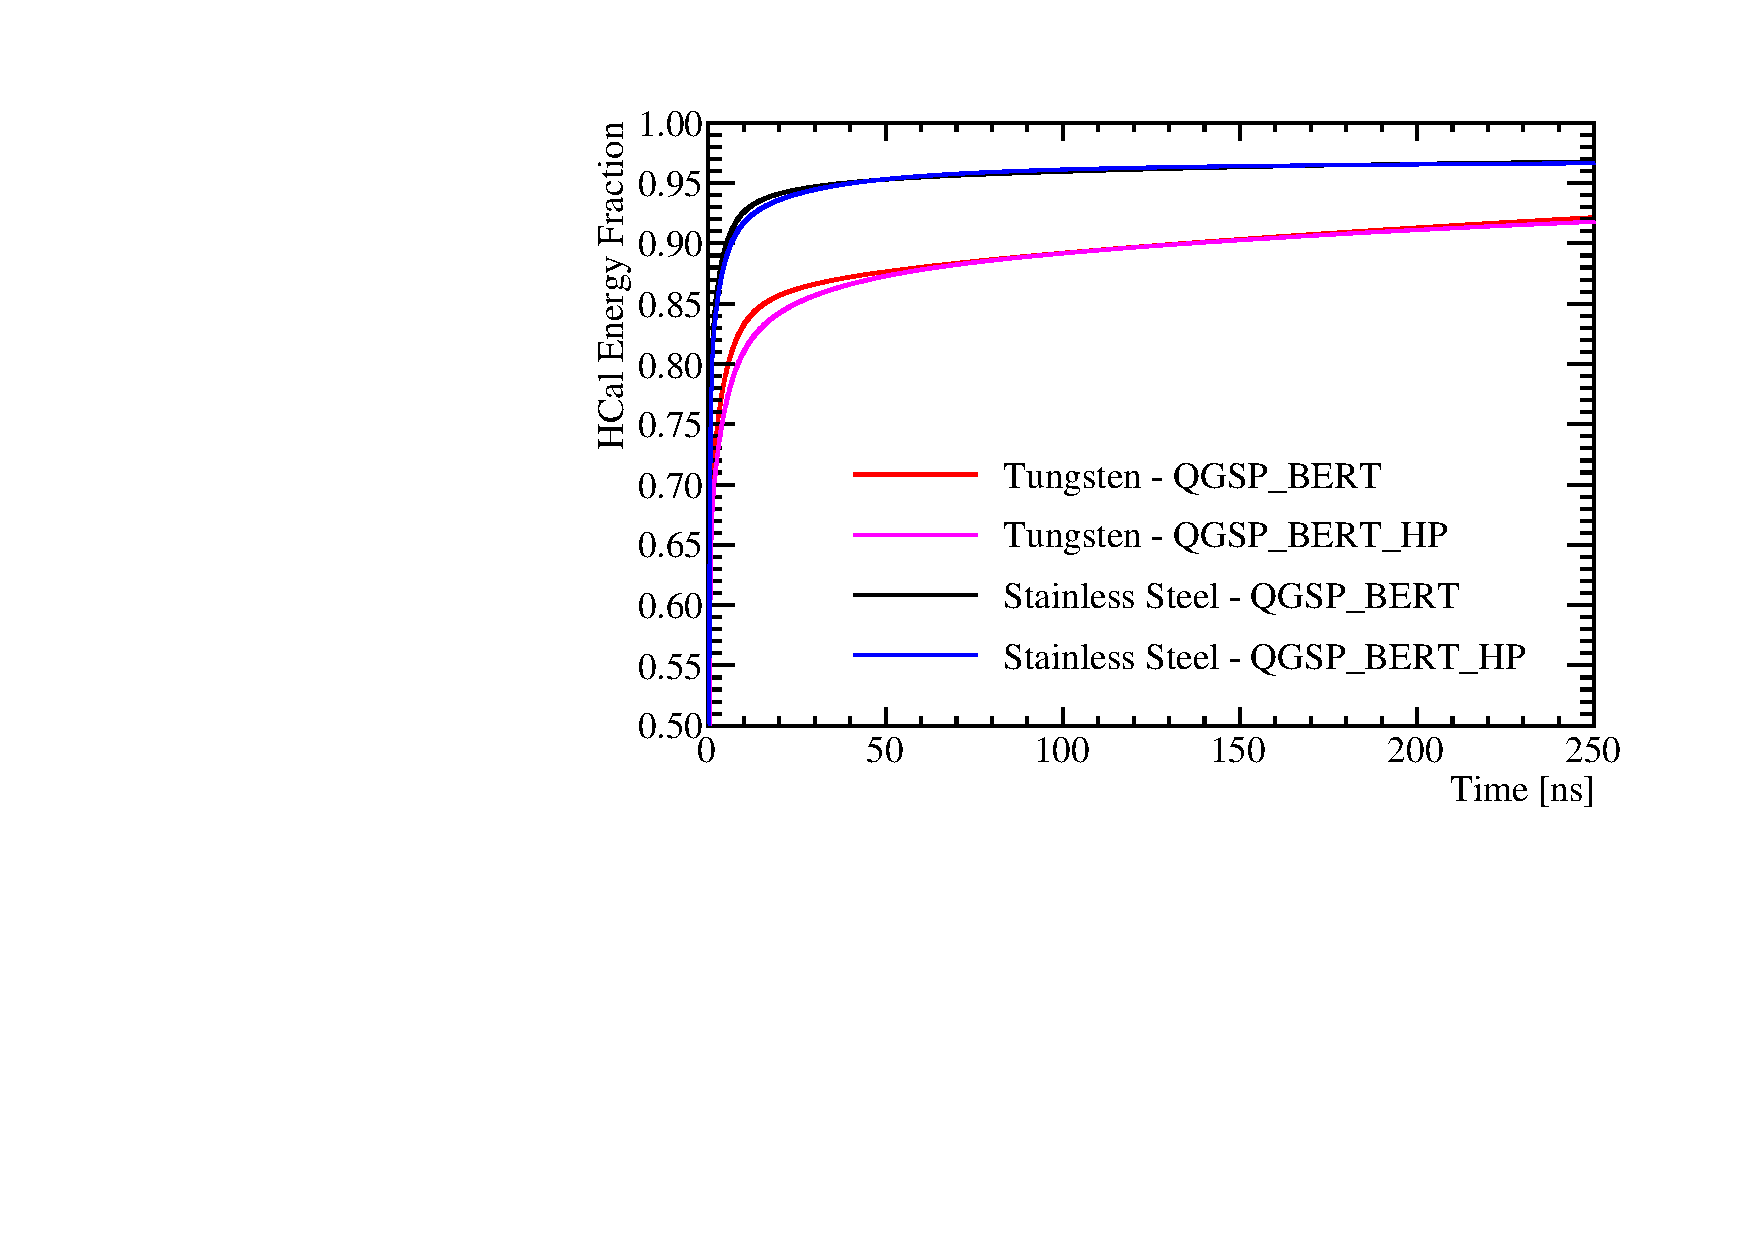
\includegraphics[width=0.5\textwidth]{OptimisationStudies/Plots/Description/HCalAbsorberMaterialTimings.pdf}
\caption[The fraction of the total calorimetric energy deposited in the HCal as a function of time for 25~GeV $\text{K}^{0}_{L}$ events using the steel and tungsten HCal options.  Results are shown for both the QGSP\_BERT and QGSP\_BERT\_HP physics lists.  The calorimeter hit times have been corrected for straight line time of flight to the impact point.]{The fraction of the total calorimetric energy deposited in the HCal as a function of time for 25~GeV $\text{K}^{0}_{L}$ events using the steel and tungsten HCal options.  Results are shown for both the QGSP\_BERT and QGSP\_BERT\_HP physics lists.  The calorimeter hit times have been corrected for straight line time of flight to the impact point.}
\label{fig:hcalabsmaterialtiming}
\end{figure} 

Table \ref{table:erhcalabsmaterial} shows the energy resolution for 50~GeV $\text{K}^{0}_{L}$s obtained using the nominal ILD detector model with various HCal absorber materials and GEANT4 physics lists.  In comparison to steel, tungsten option offers an $\sim 8\%$ improvement in the energy resolution for 50~GeV neutral hadrons (using the QGSP\_BERT\_HP physics list).  This can be attributed to differences in the nuclear structure of the two materials, which will lead to different developments of the hadronic showers within them. For example, the energy losses to nuclear binding energies are smaller in tungsten than steel, as the target nucleons are less stable than in iron, therefore, less energy is needed to liberate them.  This will lead to a larger signal for tungsten and a reduction in the energy resolution in comparison to steel.  The results of table \ref{table:erhcalabsmaterial} also indicate that the addition of the high precision neutron package was not important for this study.  

\begin{table}[h!]
\centering
\begin{tabular}{ l c }
\hline
HCal Option & Energy Resolution [\%] \\
\hline
Steel, QGSP\_BERT & $8.8\pm0.2$ \\
Steel, QGSP\_BERT\_HP & $9.0\pm0.3$ \\
Tungsten, QGSP\_BERT & $8.3\pm0.2$ \\
Tungsten, QGSP\_BERT\_HP & $8.3\pm0.2$ \\
\hline
\end{tabular}
\caption[The energy resolution for 50~GeV $\text{K}^{0}_{L}$s obtained using the nominal ILD detector with various HCal absorber materials and GEANT4 physics lists.  A 100~ns timing cut was applied to the steel and tungsten HCal options in these simulations.]{The energy resolution for 50~GeV $\text{K}^{0}_{L}$s obtained using the nominal ILD detector with various HCal absorber materials and GEANT4 physics lists.  A 100~ns timing cut was applied to the steel and tungsten HCal options in these simulations.}
\label{table:erhcalabsmaterial}
\end{table}

It should be emphasised that the HCal hit energy truncation, as described in chapter \ref{chap:energyestimators}, used for the tungsten and steel HCal options differs because tungsten contains a larger number of radiation lengths per nuclear interaction length than steel does.  As the HCal primarily measures hadronic showers, one may naively expect the number of radiation lengths in the HCal to be irrelevant, given both options have the same number of nuclear interaction lengths.  However, this is not the case because all hadronic showers have an electromagnetic component generated by the decays of hadrons to photons, e.g  $\pi^{0} \rightarrow \gamma \gamma$ and $\eta \rightarrow \gamma \gamma$.  This leads to hadronic showers depositing more energy per calorimeter hit in tungsten than in steel and makes retuning the HCal hit energy truncation a necessity.  As expected, the truncation used for tungsten, 5~GeV, is larger than for steel, 1~GeV, because of the increased average hit energy.

Table \ref{table:jerhcalabsmaterial} shows the jet energy resolutions for selected jet energies obtained using the nominal ILD detector with various HCal absorber materials and GEANT4 physics lists.  These results indicate that steel outperforms tungsten as the HCal absorber material.  The magnitude of the improvement offered using steel grows as the jet energy increases; the jet energy resolution is $\sim 3\%$ better for the steel option for 45~GeV jets, while for 250~GeV jets the improvement is $\sim 11\%$.  The intrinsic energy resolution and confusion contributions to the jet energy resolution for 45 and 250~GeV jets are shown in table \ref{table:jerbdhcalabsmaterial}.  The intrinsic energy resolution contribution to the jet energy resolution is almost identical for the two HCal options, which is expected because the $\text{K}^{0}_{L}$ energy resolution was only slightly better for the tungsten option.  The tungsten option is unlikely to give a significantly better intrinsic energy resolution because only the small fraction of jet energy associated with neutral hadrons is measured in the HCal. The confusion contribution to the jet energy resolution is larger for tungsten than for steel; for 250~GeV jets the confusion contribution is $\sim 3.4\%$ in tungsten and only $\sim 3.0\%$ in steel.  The larger confusion contribution is expected for the tungsten option because hadronic showers are generally wider in tungsten.  The transverse profile of hadronic showers in the two HCal options is illustrated in figure \ref{fig:transversedistanceshower}, which shows the normalised distribution of the energy weighted transverse distance from the shower axis to the calorimeter hits for 50~GeV hadronic showers for both the steel and tungsten HCal options.  Increasing the average hadronic shower width makes resolving individual particle showers in a dense jet environment more challenging, which means more calorimetric energy deposits will be incorrectly clustered together.  This in turn results in incorrect associations being made between calorimetric energy deposits and charged particle tracks i.e. an increased confusion contribution.  Again, the use of the QGSP\_BERT\_HP physics list, as opposed to QGSP\_BERT, made a minimal impact on these results.

\begin{table}[h!]
\centering
\begin{tabular}{ l c c c c }
\hline
 & \multicolumn{4}{c}{Jet Energy Resolution [\%]} \\
HCal Option & 45~GeV & 100~GeV & 180~GeV & 250~GeV \\
\hline
Steel, QGSP\_BERT & $3.65 \pm 0.05$ &$2.88 \pm 0.04$ &$2.85 \pm 0.04$ &$2.97 \pm 0.05$ \\
Steel, QGSP\_BERT\_HP & $3.67 \pm 0.05$ &$2.92 \pm 0.04$ &$2.86 \pm 0.04$ &$3.03 \pm 0.04$ \\
Tungsten, QGSP\_BERT & $3.78 \pm 0.05$ & $3.12 \pm 0.04$ & $3.15 \pm 0.04$ & $3.43 \pm 0.04 |$ \\
Tungsten, QGSP\_BERT\_HP & $3.80 \pm 0.05$ & $3.08 \pm 0.04$ & $3.24 \pm 0.04$ & $3.41 \pm 0.04$ \\
%Tungsten, QGSP\_BERT & $3.67 \pm 0.05$ &$3.12 \pm 0.04$ &$3.36 \pm 0.04$ &$3.76 \pm 0.05$ \\ 1~GeV Truncation 
%Tungsten, QGSP\_BERT\_HP & $3.69 \pm 0.05$ &$3.03 \pm 0.04$ &$3.38 \pm 0.04$ &$3.80 \pm 0.05$ \\ 1~GeV Truncation
\hline
\end{tabular}
\caption[The jet energy resolution for selected jet energies obtained using the nominal ILD detector with various HCal absorber materials and GEANT4 physics lists.  A 100~ns timing cut was applied to the steel and tungsten HCal options in these simulations.]{The jet energy resolution for selected jet energies obtained using the nominal ILD detector with various HCal absorber materials and GEANT4 physics lists.  A 100~ns timing cut was applied to the steel and tungsten HCal options in these simulations.}
\label{table:jerhcalabsmaterial}
\end{table}

\begin{table}[h!]
\centering
\begin{tabular}{ l c c c c }
\hline
 & \multicolumn{4}{c}{Jet Energy Resolution [\%]} \\
 & \multicolumn{2}{c}{45~GeV} & \multicolumn{2}{c}{250~GeV} \\
HCal Option & Intrinsic & Confusion & Intrinsic & Confusion \\
\hline
Steel, QGSP\_BERT & $2.93 \pm 0.04$ & $2.16 \pm 0.06$ & $1.69 \pm 0.02$ &$2.45 \pm 0.05$ \\
Steel, QGSP\_BERT\_HP & $2.98 \pm 0.04$ &$2.15 \pm 0.06$ &$1.65 \pm 0.02$ &$2.53 \pm 0.04$ \\
Tungsten, QGSP\_BERT & $2.97 \pm 0.04$ & $2.34 \pm 0.06$ & $1.65 \pm 0.02$ & $3.01 \pm 0.05$ \\
Tungsten, QGSP\_BERT\_HP & $2.92 \pm 0.04$ & $2.42 \pm 0.06$ & $1.65 \pm 0.02$ & $2.99 \pm 0.05$ \\
\hline
\end{tabular}
\caption[The contributions to the jet energy resolution obtained using the nominal ILD detector with various HCal absorber materials and GEANT4 physics lists.  A 100~ns timing cut was applied to the steel and tungsten HCal options in these simulations.]{The contributions to the jet energy resolution obtained using the nominal ILD detector with various HCal absorber materials and GEANT4 physics lists.  A 100~ns timing cut was applied to the steel and tungsten HCal options in these simulations.}
\label{table:jerbdhcalabsmaterial}
\end{table}

\begin{figure}[h!]
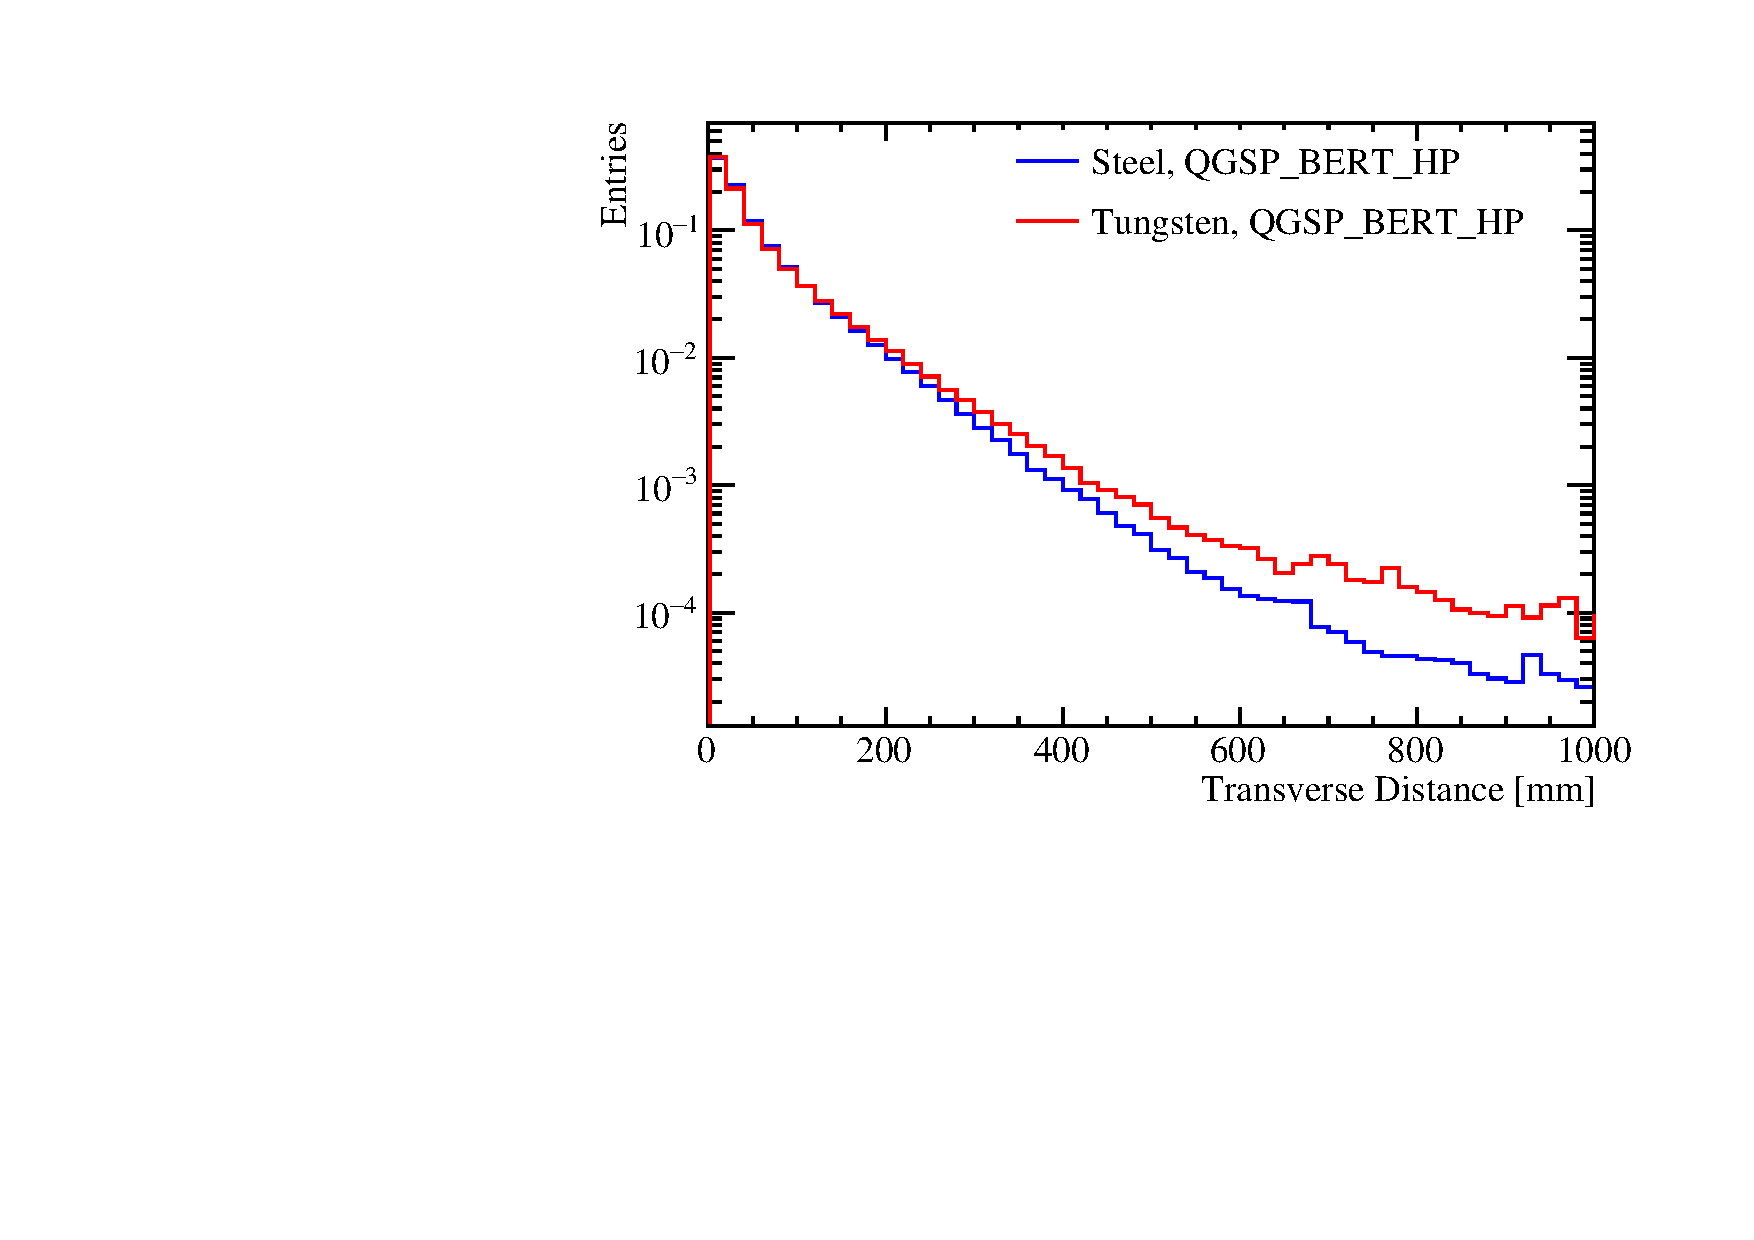
\includegraphics[width=0.5\textwidth]{OptimisationStudies/Plots/EnergyResolution/ShowerShape/Profile2.pdf}
\caption[The normalised distribution of the energy weighted transverse distance of the calorimeter hits from a 50~GeV hadronic shower to the shower axis.  The blue and red lines show the energy weighted transverse distance obtained using a steel and tungsten HCal absorber material in the ILD detector respectively.  The simulations used the QGSP\_BERT\_HP physics list.]{The normalised distribution of the energy weighted transverse distance of the calorimeter hits from a 50~GeV hadronic shower to the shower axis.  The blue and red lines show the energy weighted transverse distance obtained using a steel and tungsten HCal absorber material in the ILD detector respectively.  The simulations used the QGSP\_BERT\_HP physics list.}
\label{fig:transversedistanceshower}
\end{figure}

The impact of the choice of HCal absorber material is small on both the neutral hadron energy resolution and intrinsic energy resolution, however,  the steel HCal option outperforms the tungsten option in terms of pattern recognition confusion.  When examining the mechanical properties of steel and tungsten, it is clear that steel has a significant advantage over tungsten in terms of rigidity \cite{Linssen:2012hp}.  This means that fewer support structures would be required for the calorimeter leading to less dead material and better performance, which makes steel the preferred option.

%========================================================================================
%========================================================================================

\section{Global Detector Parameters}
The overall detector size and the magnetic field strength are major cost drivers for the ILD detector.  Both will affect the jet energy resolution and studies showing their impact on detector performance are presented here.

%========================================================================================

\subsection{The Magnetic Field Strength}
\label{sec:bfield}
In the particle flow paradigm the momentum of charged particles is obtained through the curvature of their trajectory as they bend in the magnetic field.  Therefore, the magnetic field is an integral element for the successful application of particle flow calorimetry.  Furthermore, the magnetic field deflects charged particles away from neutral particles in jets.  The stronger the magnetic field, the larger the average separation between the calorimetric energy deposits made by charged and neutral particles in jets, which reduces the effect of confusion.  Therefore, it is expected that a stronger magnetic field will lead to better jet energy resolutions through a reduction of the confusion contribution to the jet energy resolution.  

Detector models were simulated where the magnetic field was varied from 1.0 to 5.0~T in steps of 0.5~T and the resulting jet energy resolutions  are shown in figure \ref{fig:bfield}.  The larger the magnetic field strength, the better the jet energy resolution.  Increasing the magnetic field strength from 1.0 to 5.0~T improves the jet energy resolution for 250~GeV jets by $\sim 25 \%$.  The higher the jet energy, the stronger the dependence of the jet energy resolution on the magnetic field strength.  

\begin{figure}[h!]
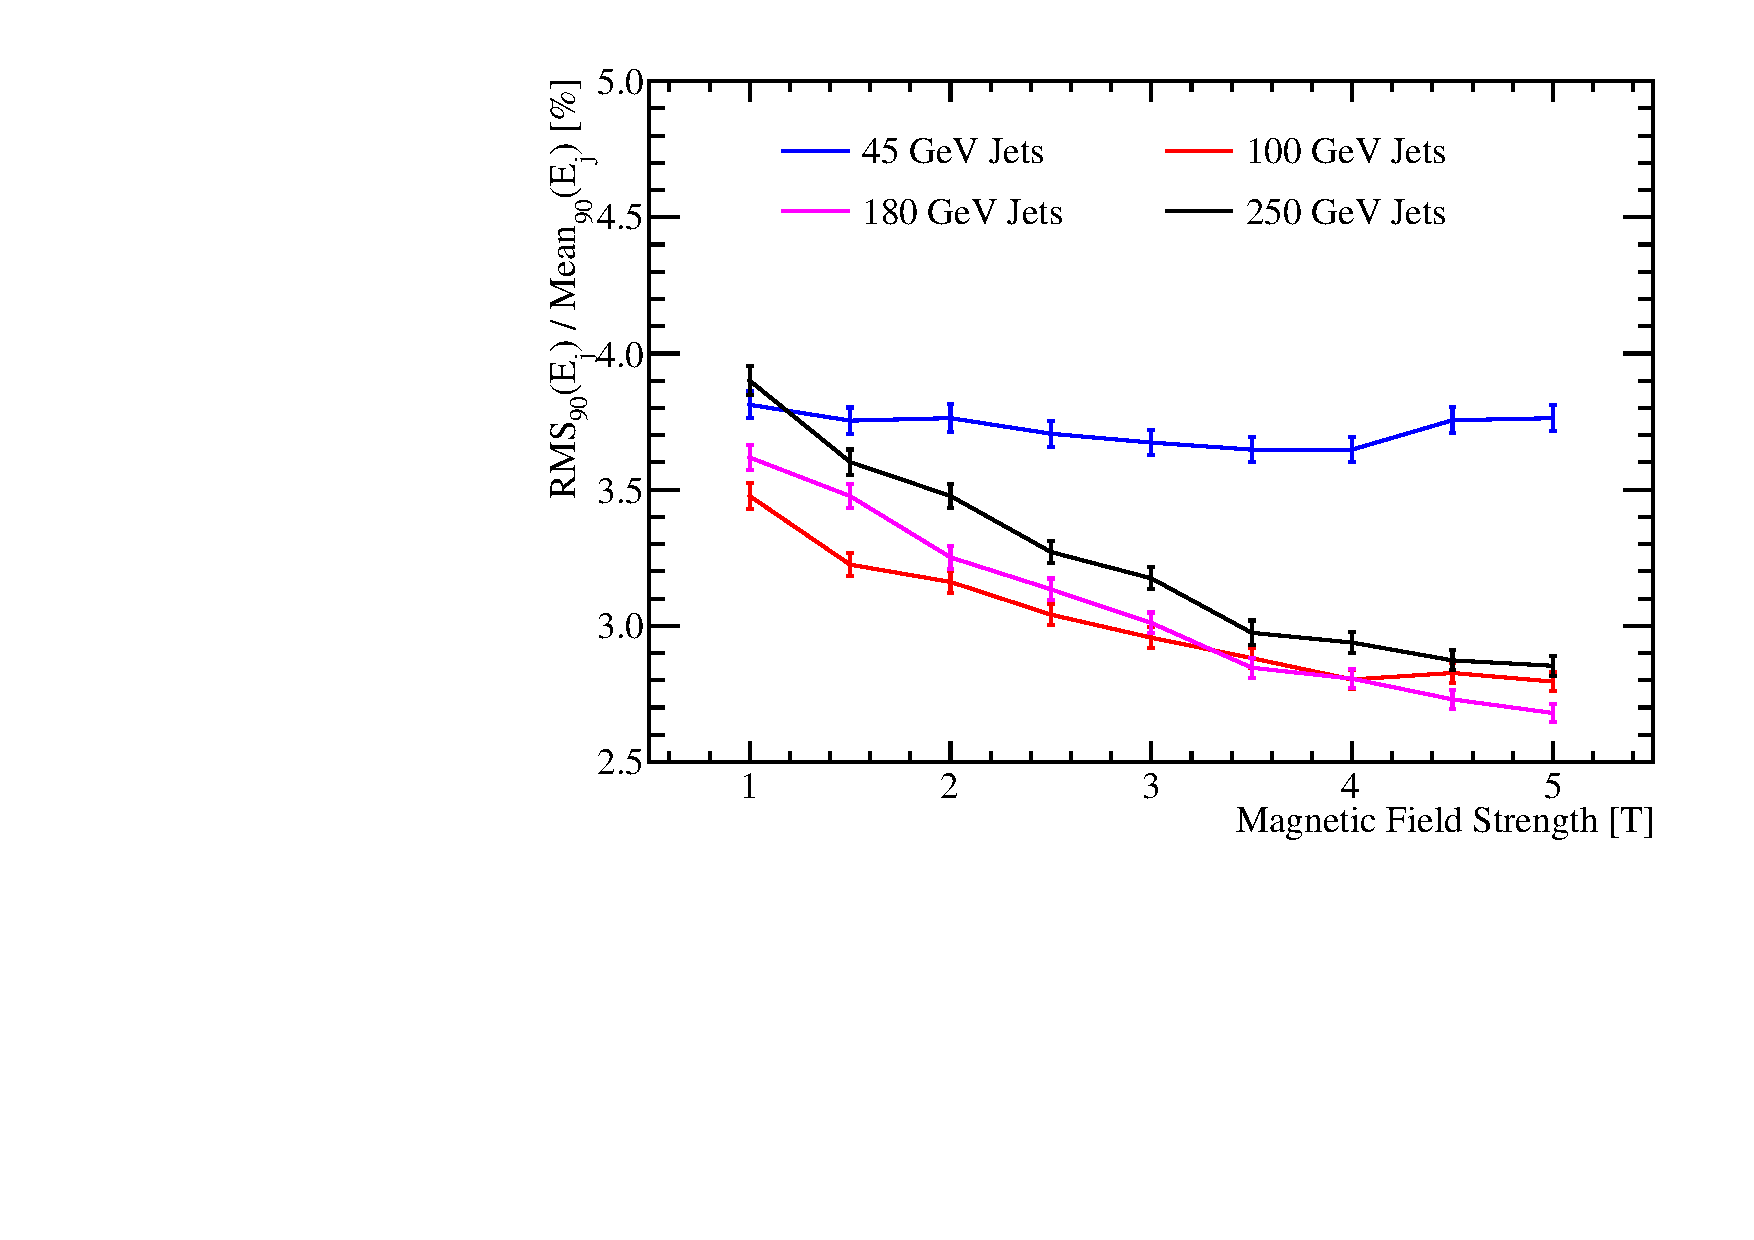
\includegraphics[width=0.5\textwidth]{OptimisationStudies/Plots/JetEnergyResolutions/JER_vs_MagneticFieldStrength.pdf}
\caption[The jet energy resolution using the nominal ILD detector as a function of the magnetic field strength for various jet energies.]{The jet energy resolution using the nominal ILD detector as a function of the magnetic field strength for various jet energies.}
\label{fig:bfield}
\end{figure}

Figure \ref{fig:bfieldbreak} shows the breakdown of the jet energy resolution into the various contributions.  As expected, there is a reduction in the confusion contribution with increasing magnetic field strength.  Furthermore, there is a reduction in intrinsic energy resolution with increasing magnetic field strength for low energy jets.  This is most likely due to particles being directed into the forward region of the detector.  When a charged particle passes through a magnetic field it will, assuming no energy losses, traverse a helix.  The radius of curvature, $R$, of that helix is given by 
%
\begin{equation}
R = \frac{p_{\text{T}}}{qB} \text{ ,}
\end{equation}
%
where $p_{\text{T}}$ is the transverse momentum of the charged particle with respect to the magnetic field, $q$ is the electric charge of the particle and $B$ is the magnetic field strength.  When the magnetic field strength increases, the radius of curvature for charged particles will decrease and more low charged particles will be directed toward the forward regions of the detector.  As the tracking coverage in the forward region of the detector is worse in the central region \cite{Behnke:2013lya}, increasing the magnetic field strength leads to fewer charged particles being reconstructed, which is illustrated in figure \ref{fig:bfieldchargedparticles}, and a degradation in the energy resolution.  For high jet energies, low transverse momentum charged particles will still get directed to the forward regions of the detector, however, these contribute fractionally less energy to the total reconstructed energy.  Therefore, the trend of worsening intrinsic energy resolution with increasing magnetic field strength is less pronounced as the jet energy grows.  

At high jet energies, reducing the magnetic field strength appears to degrade the intrinsic energy resolution; the intrinsic energy resolution for 250~GeV jets goes from $\sim1.8\%$ to $\sim2.1\%$ when reducing the magnetic field strength from 5.0~T to 1.0~T.  This trend is due to an artefact in the definition of the intrinsic energy resolution for jets meaning it is not a genuine effect.  The intrinsic energy resolution is highly non-trivial to determine; Monte-Carlo (MC) information is used to make all associations between charged particle tracks and clusters of calorimeter hits as follows:

\begin{enumerate}
\item Each calorimeter hit is associated to the MC particle that deposits the largest amount of energy in that hit;
\item Clusters of calorimeter hits formed by the same MC particle are clustered together;
\item Each charged particle track is associated to the MC particle that produced it;
\item Clusters of calorimeter hits are associated to charged particle tracks if they are made by the same MC particle.
\end{enumerate}

This procedure assumes that only one MC particle deposits significant energy per calorimeter hit.  If multiple MC particles deposit significant energy in the same calorimeter hit, this assumption breaks down and errors are made when associating charged particle tracks to calorimetric energy deposits.  These errors cause the same double counting and omission of energy deposits as confusion does, however, they have a smaller effect because multiple MC particles deposit significant energy in the same calorimeter hit is rare in finely segmented calorimeters.  As the overlap of particle showers within the calorimeter grows, as it does for high energy jets when reducing the magnetic field, the intrinsic energy resolution appears to get worse because of this confusion-like effect.  Because this effect is small in comparison to changes in the confusion contribution, the overall dependence of the detector performance on the magnetic field strength can be confidently quantified.  

\begin{figure}[h!]
\subfloat[]{\label{fig:bfield45break}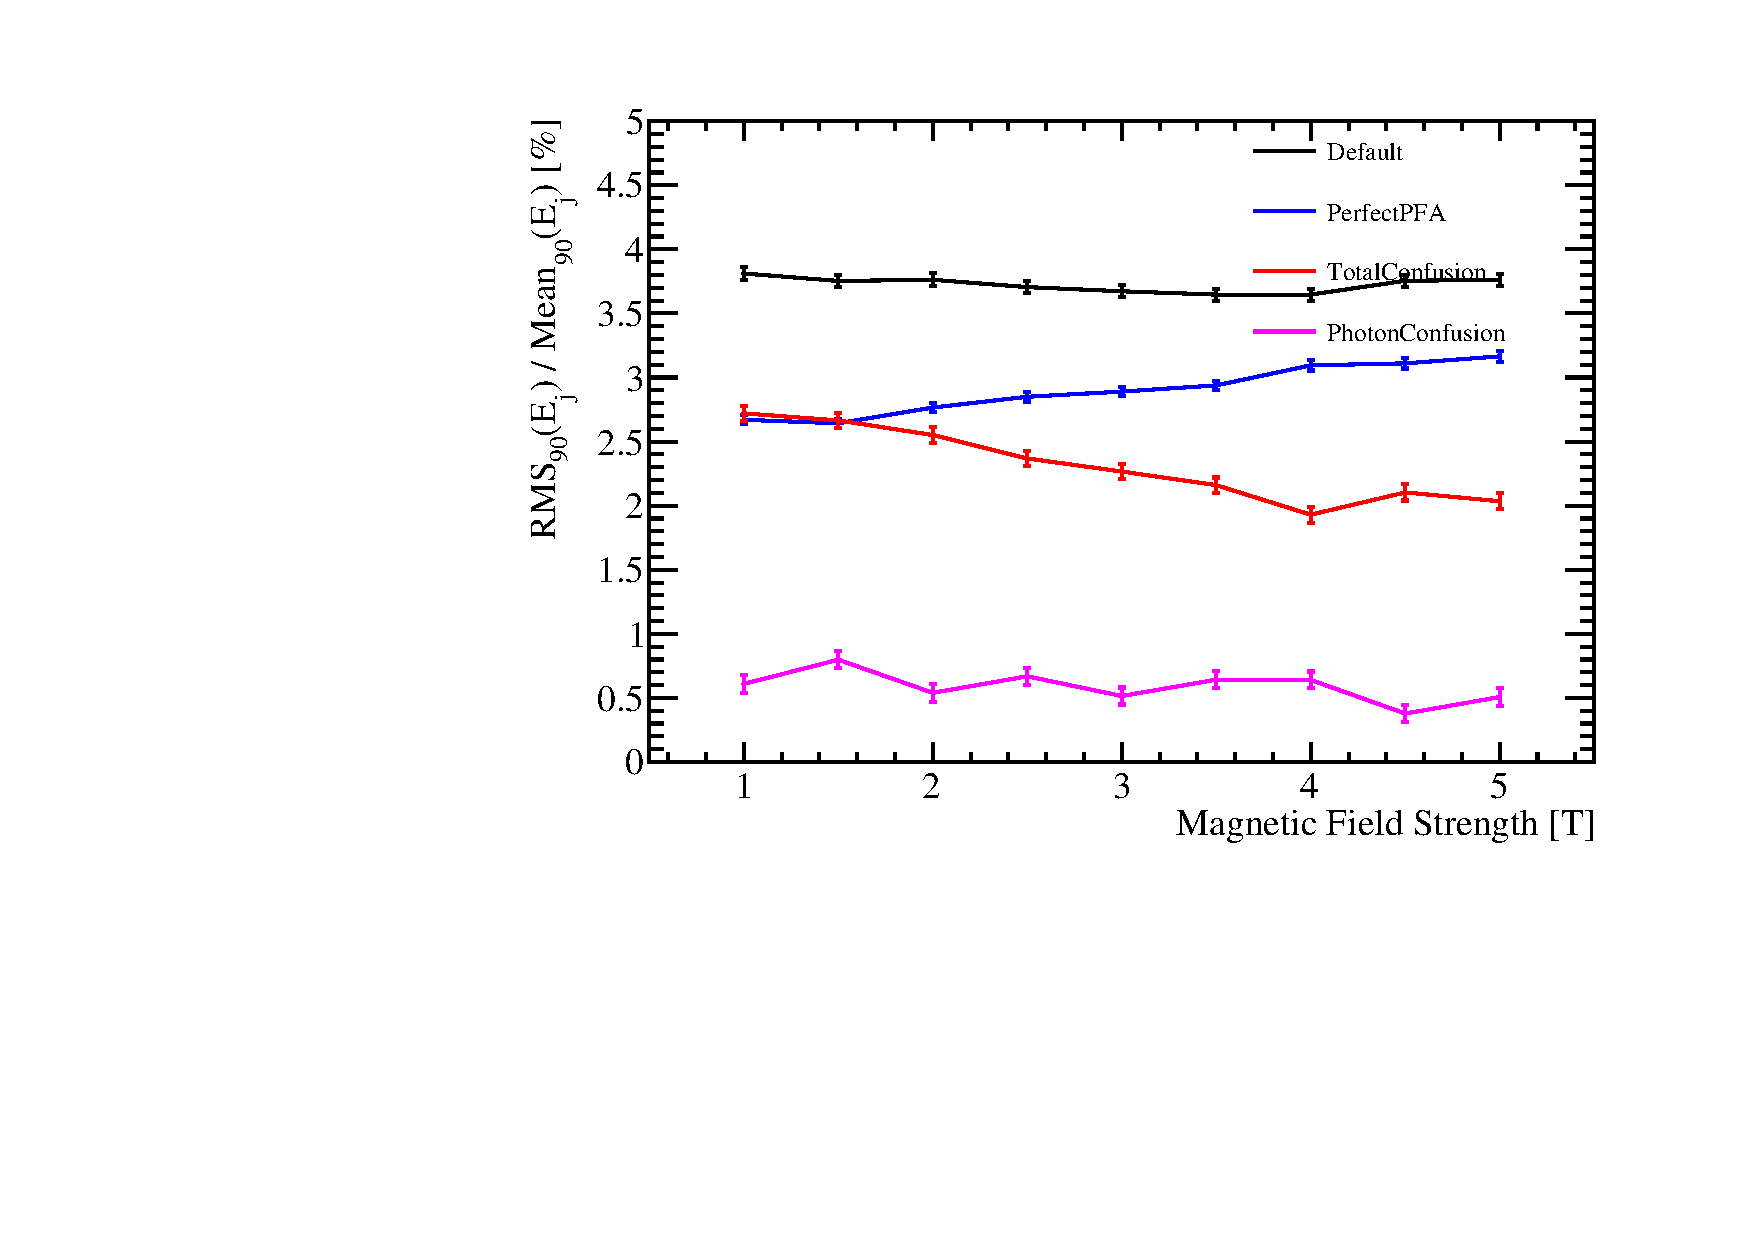
\includegraphics[width=0.5\textwidth]{OptimisationStudies/Plots/JetEnergyResolutions/JER_vs_MagneticFieldStrength_91GeV_DiJet_Breakdown.pdf}}
\subfloat[]{\label{fig:bfield250break}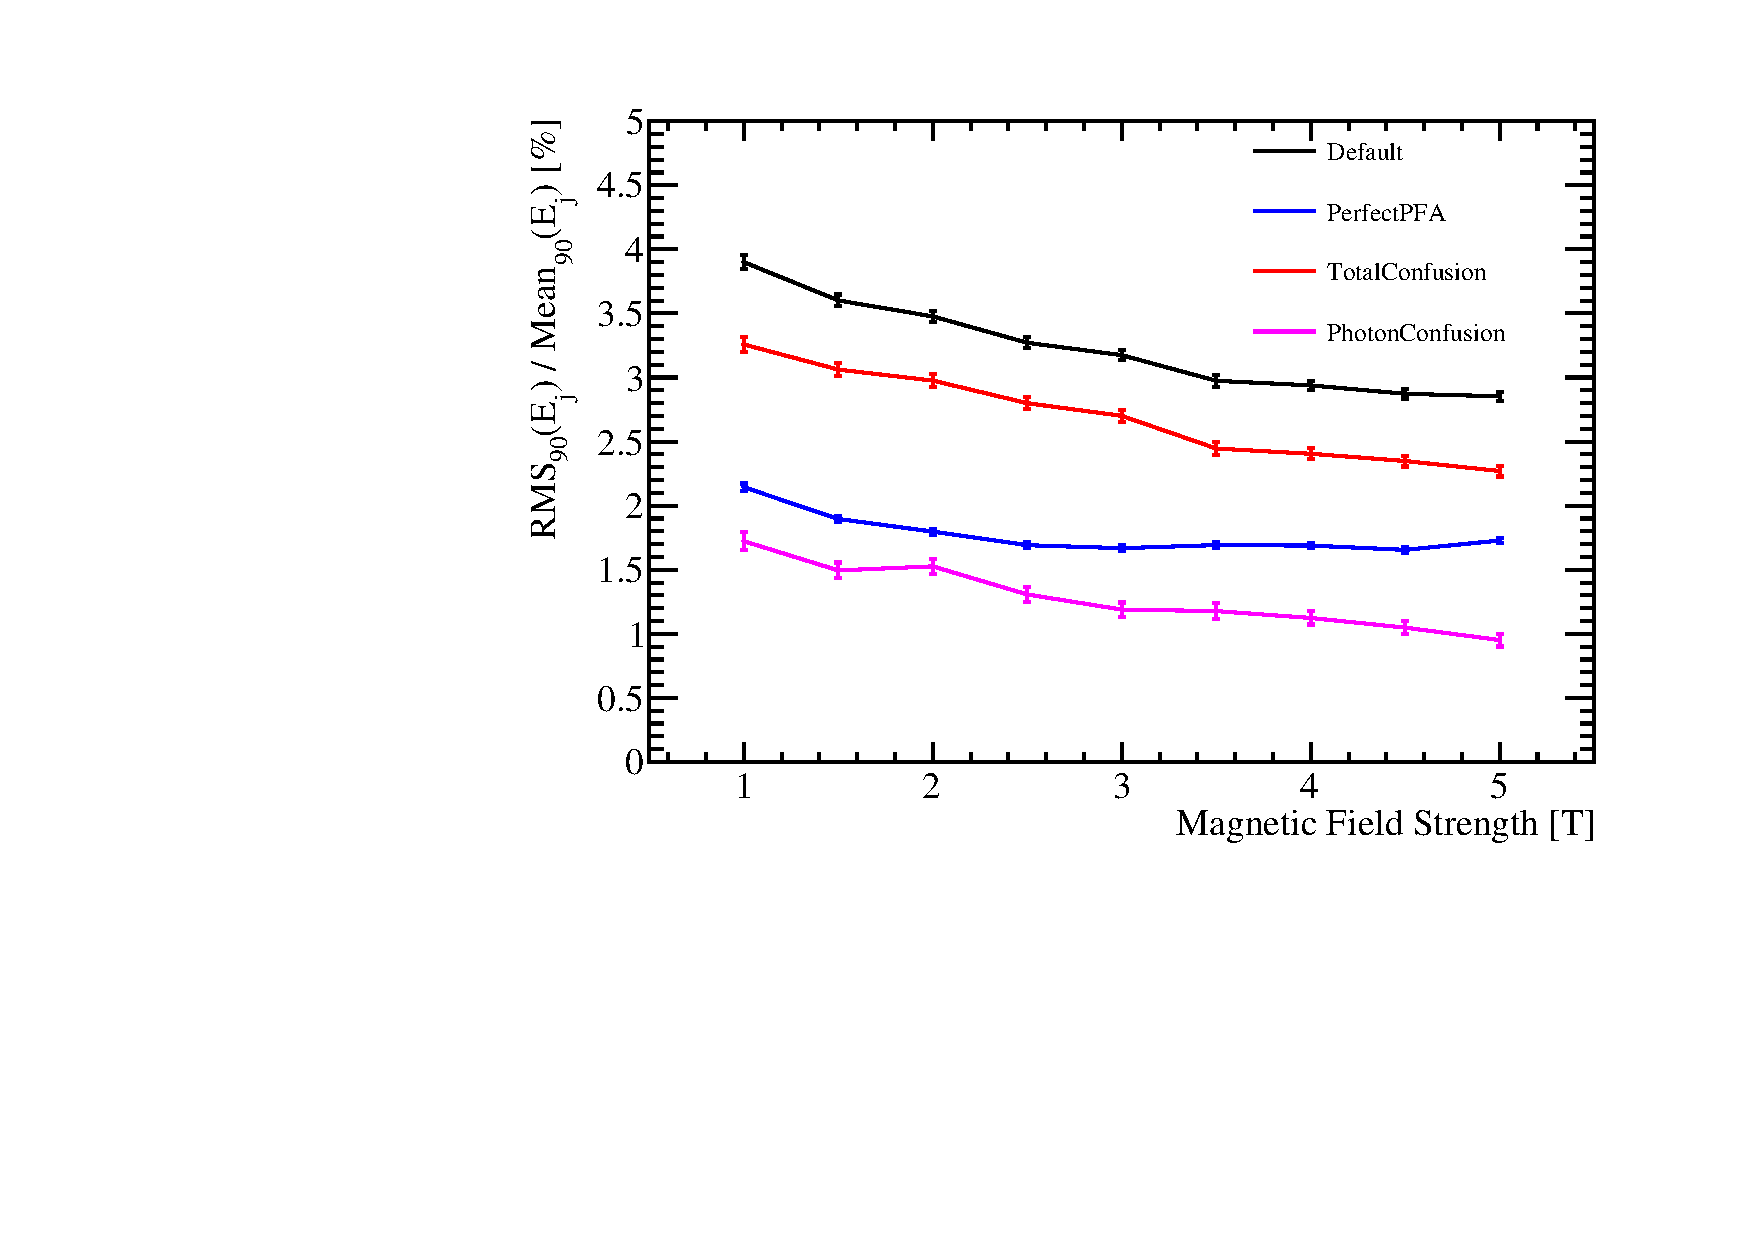
\includegraphics[width=0.5\textwidth]{OptimisationStudies/Plots/JetEnergyResolutions/JER_vs_MagneticFieldStrength_500GeV_DiJet_Breakdown.pdf}}
\caption[Contributions to the jet energy resolution shown as function of the magnetic field strength using the nominal ILD detector model for \protect\subref{fig:bfield45break} 45~GeV jets and \protect\subref{fig:bfield250break} 250~GeV jets.  The black curves correspond to the standard reconstruction, the blue curves to the intrinsic energy resolution contribution to the jet energy resolution, the red curves to the confusion contribution to the jet energy resolution and the magenta curves to the confusion contribution to the jet energy resolution related solely to photon reconstruction.]{Contributions to the jet energy resolution shown as function of the magnetic field strength using the nominal ILD detector model for \protect\subref{fig:bfield45break} 45~GeV jets and \protect\subref{fig:bfield250break} 250~GeV jets.  The black curves correspond to the standard reconstruction, the blue curves to the intrinsic energy resolution contribution to the jet energy resolution, the red curves to the confusion contribution to the jet energy resolution and the magenta curves to the confusion contribution to the jet energy resolution related solely to photon reconstruction.}
\label{fig:bfieldbreak}
\end{figure}

\begin{figure}[h!]
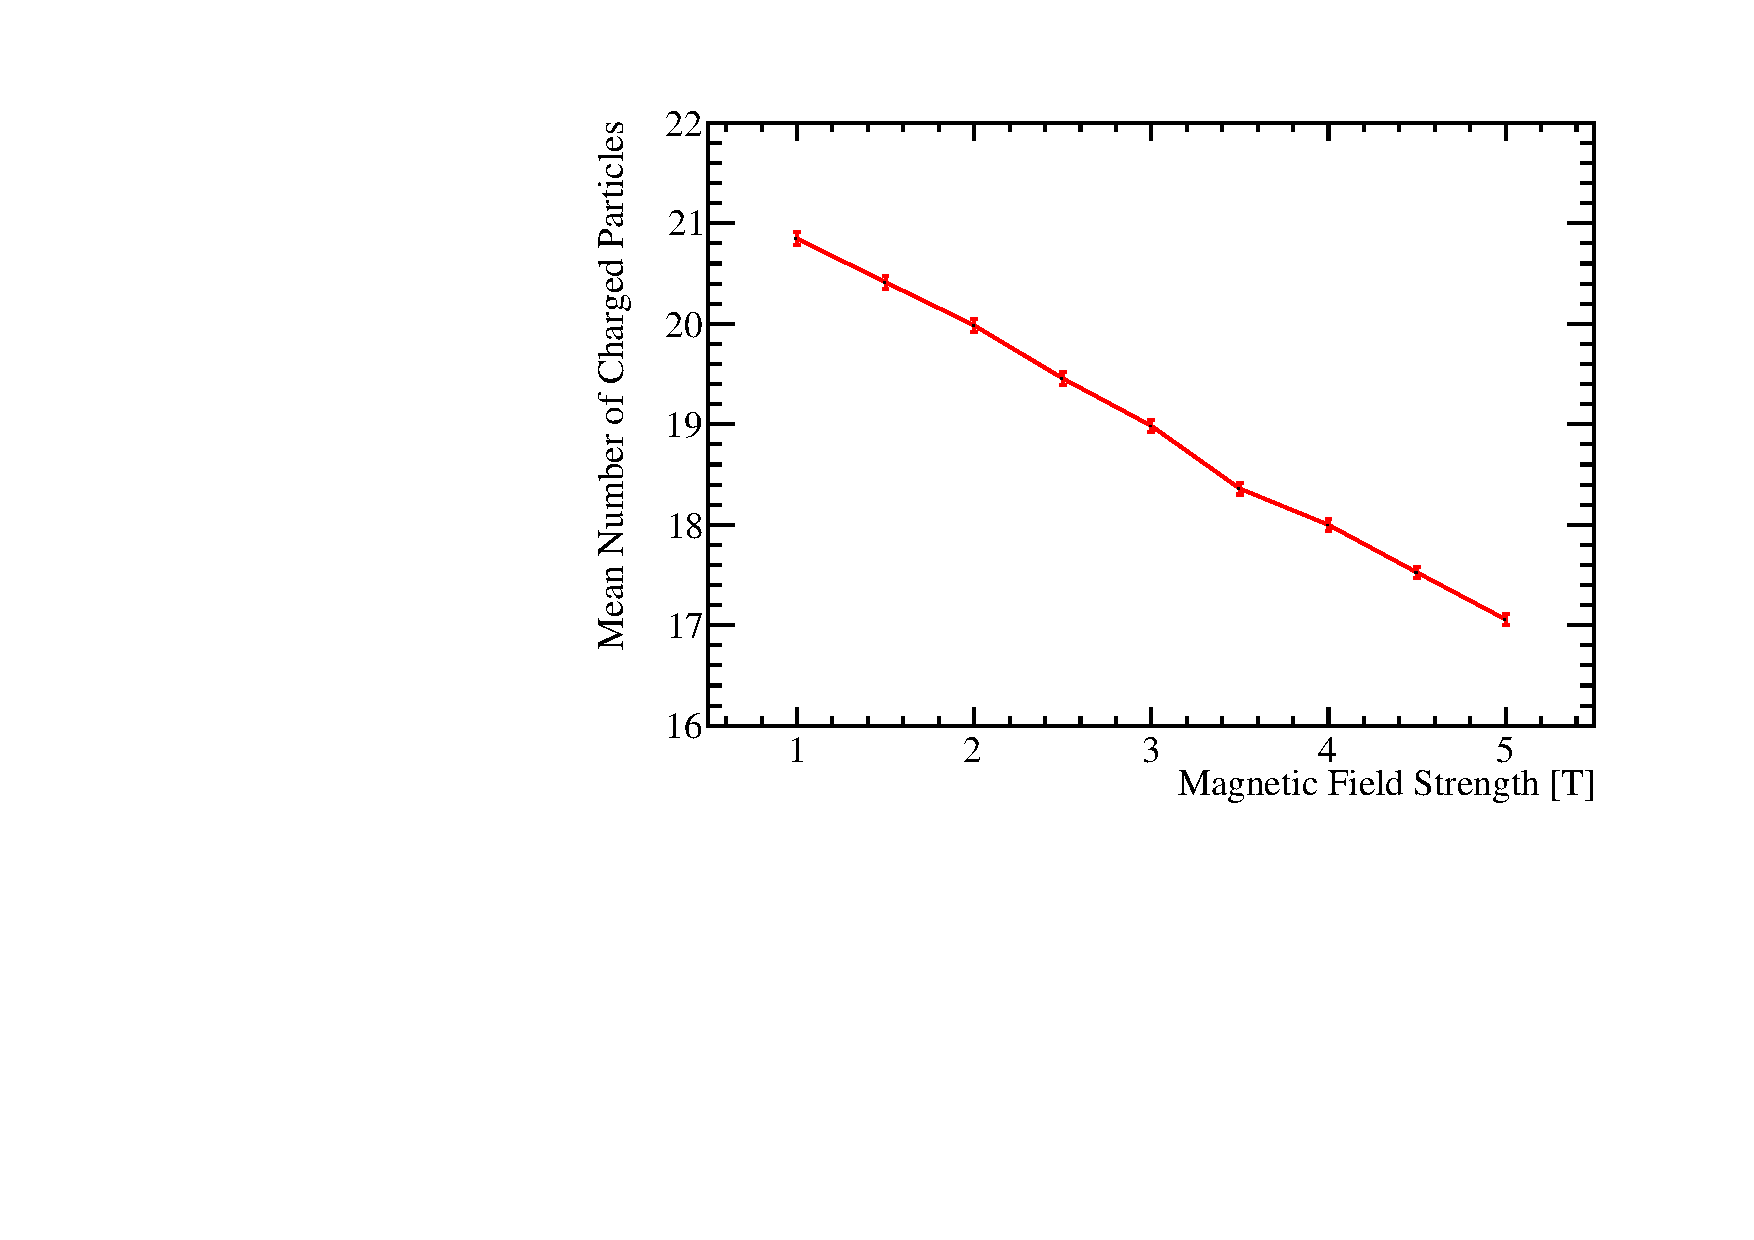
\includegraphics[width=0.5\textwidth]{OptimisationStudies/Plots/Description/BField/BFieldNumbers_91GeV_Z_uds.pdf}
\caption[The mean number of reconstructed charged particles as a function of the magnetic field strength for 91~GeV Z$\rightarrow$uds di-jet events.  The nominal ILD detector model was used and the pattern recognition has been fully cheated using the MC information.]{The mean number of reconstructed charged particles as a function of the magnetic field strength for 91~GeV Z$\rightarrow$uds di-jet events.  The nominal ILD detector model was used and the pattern recognition has been fully cheated using the MC information.}
\label{fig:bfieldchargedparticles}
\end{figure}

In summary, increasing the magnetic field strength is beneficial to the jet energy resolution because it reduces confusion from associating tracks to calorimetric energy deposits from charged particles.  The intrinsic energy resolution is also dependent upon the magnetic field strength, however, the effect is small in comparison to the confusion.  Although a magnetic field of 1.5~T would give good enough performance to be able to separate the hadronic decays of W and Z bosons, i.e. $\sigma_{E}/E \lesssim 3.8\%$ \cite{arXiv:0907.3577}, at the energies considered, increasing the field strength further significantly improves the detector performance.

%========================================================================================

\subsection{Inner ECal Radius}
The impact on the jet energy resolution of the overall size of the detector was studied by simulating detector models where the ECal inner radius was altered.  The ECal inner radii considered were 1208, 1408, 1608, 1808 (nominal) and 2008~mm.  

Figure \ref{fig:ecalinnerr} shows the dependence of the jet energy resolution on the ECal inner radius.  Increasing the ECal inner radius increases the separation between particles as they enter the calorimeters, which reduced the effect of confusion and improves the jet energy resolution.  As confusion is more dominant at higher energies, the benefits to using a larger ECal radius grow with increasing jet energy; increasing the ECal inner radius from 1208~mm to 2008~mm improves the jet energy resolution by $\sim 9\%$ for 45~GeV jets, but by $\sim 25\%$ for 250~GeV jets.  Figure \ref{fig:ecalinnerrbreak} shows the decomposition of the jet energy resolution into its different component.  These results explicitly show a reduction in confusion with increasing ECal inner radius; the confusion contribution goes from $\sim 3.4\%$ to $\sim 2.4\%$ when increasing the ECal inner radius from 1208~mm to 2008~mm.  The intrinsic energy resolution of the detectors shows no strong dependence on the inner ECal radius.  The apparent degradation in intrinsic energy resolution at low ECal inner radii is an artefact of the association of a single MC particle per calorimeter cell when running the cheated pattern recognition as explained in section \ref{sec:bfield}.  The dominant effect driving the jet energy resolution is, as expected, the confusion.  

\begin{figure}[h!]
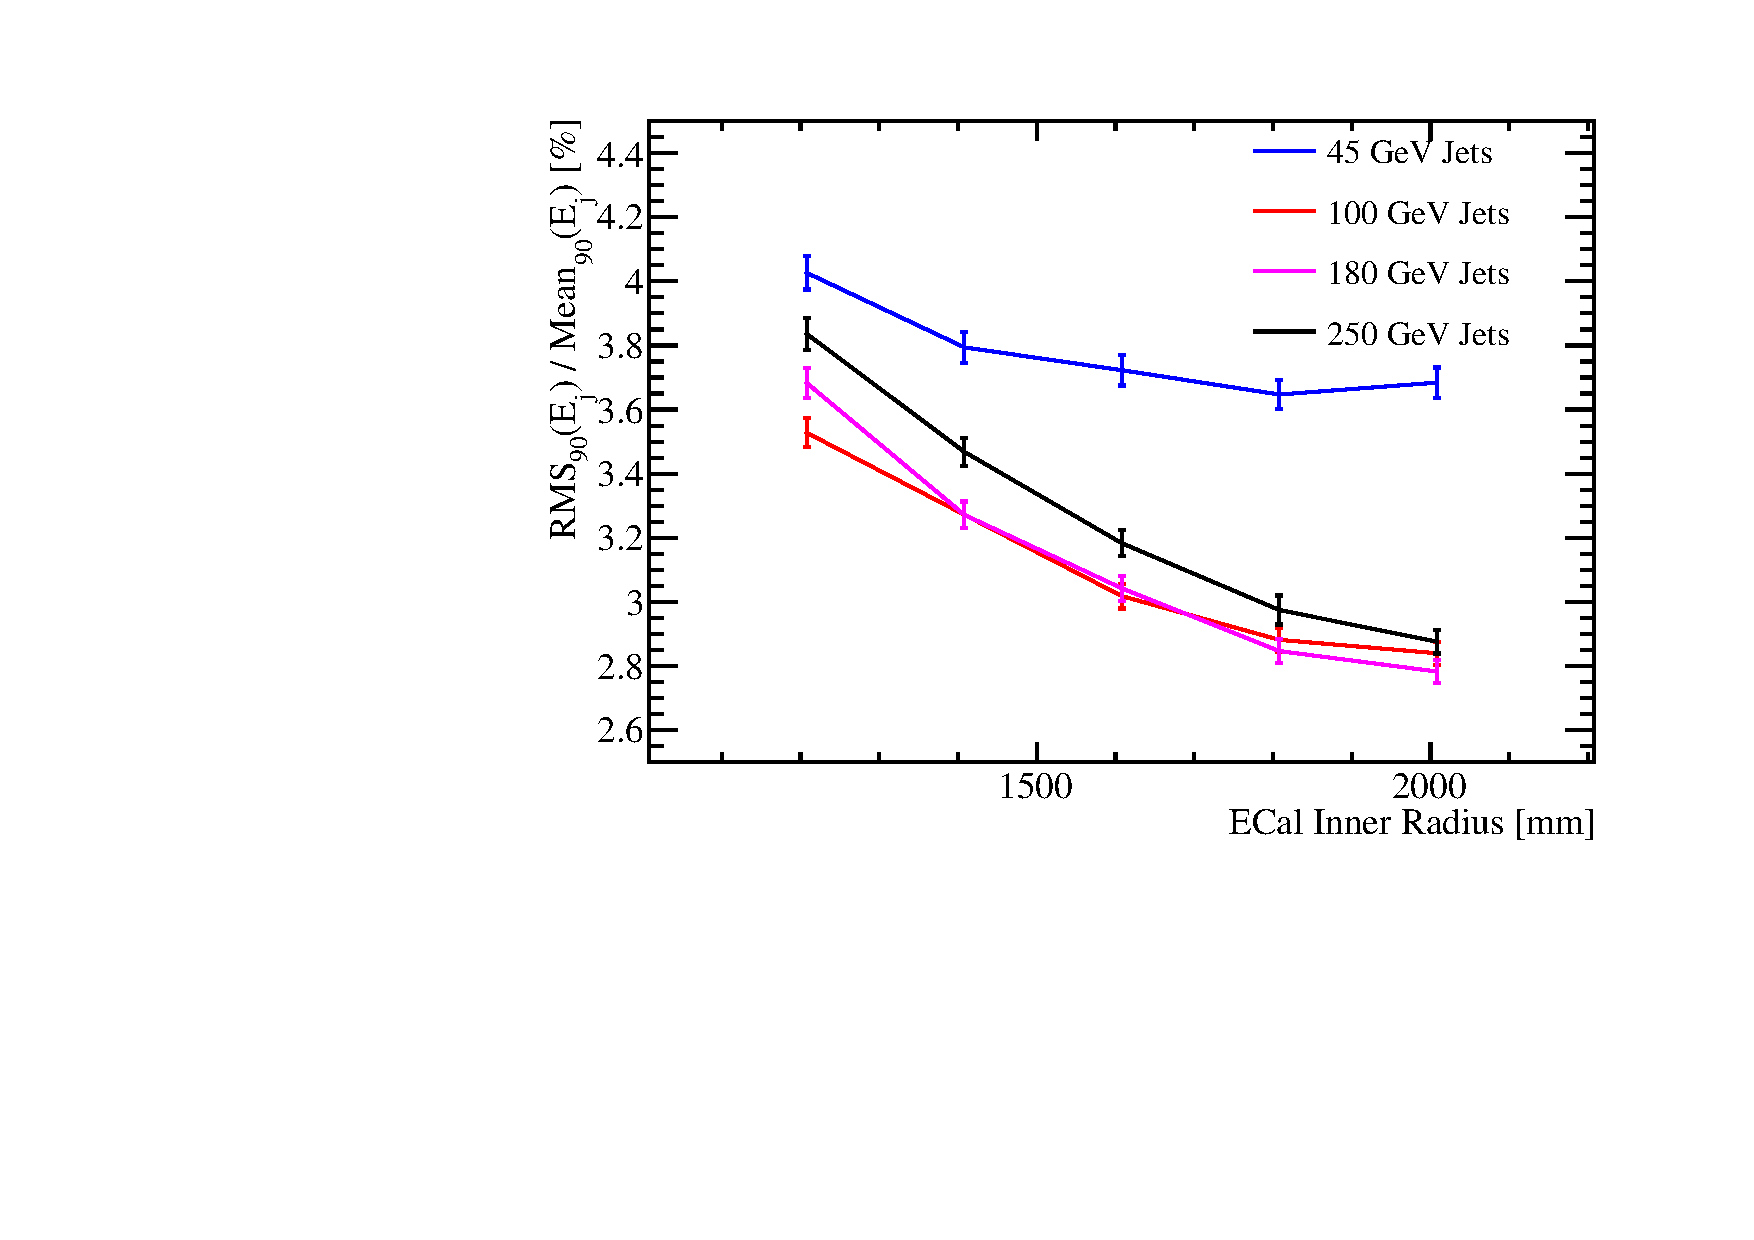
\includegraphics[width=0.5\textwidth]{OptimisationStudies/Plots/JetEnergyResolutions/JER_vs_ECalInnerRadius.pdf}
\caption[The jet energy resolution using the nominal ILD detector as a function of the ECal inner radius for various jet energies.]{The jet energy resolution using the nominal ILD detector as a function of the ECal inner radius for various jet energies.}
\label{fig:ecalinnerr}
\end{figure}

\begin{figure}[h!]
\subfloat[]{\label{fig:ecalinnerr45break}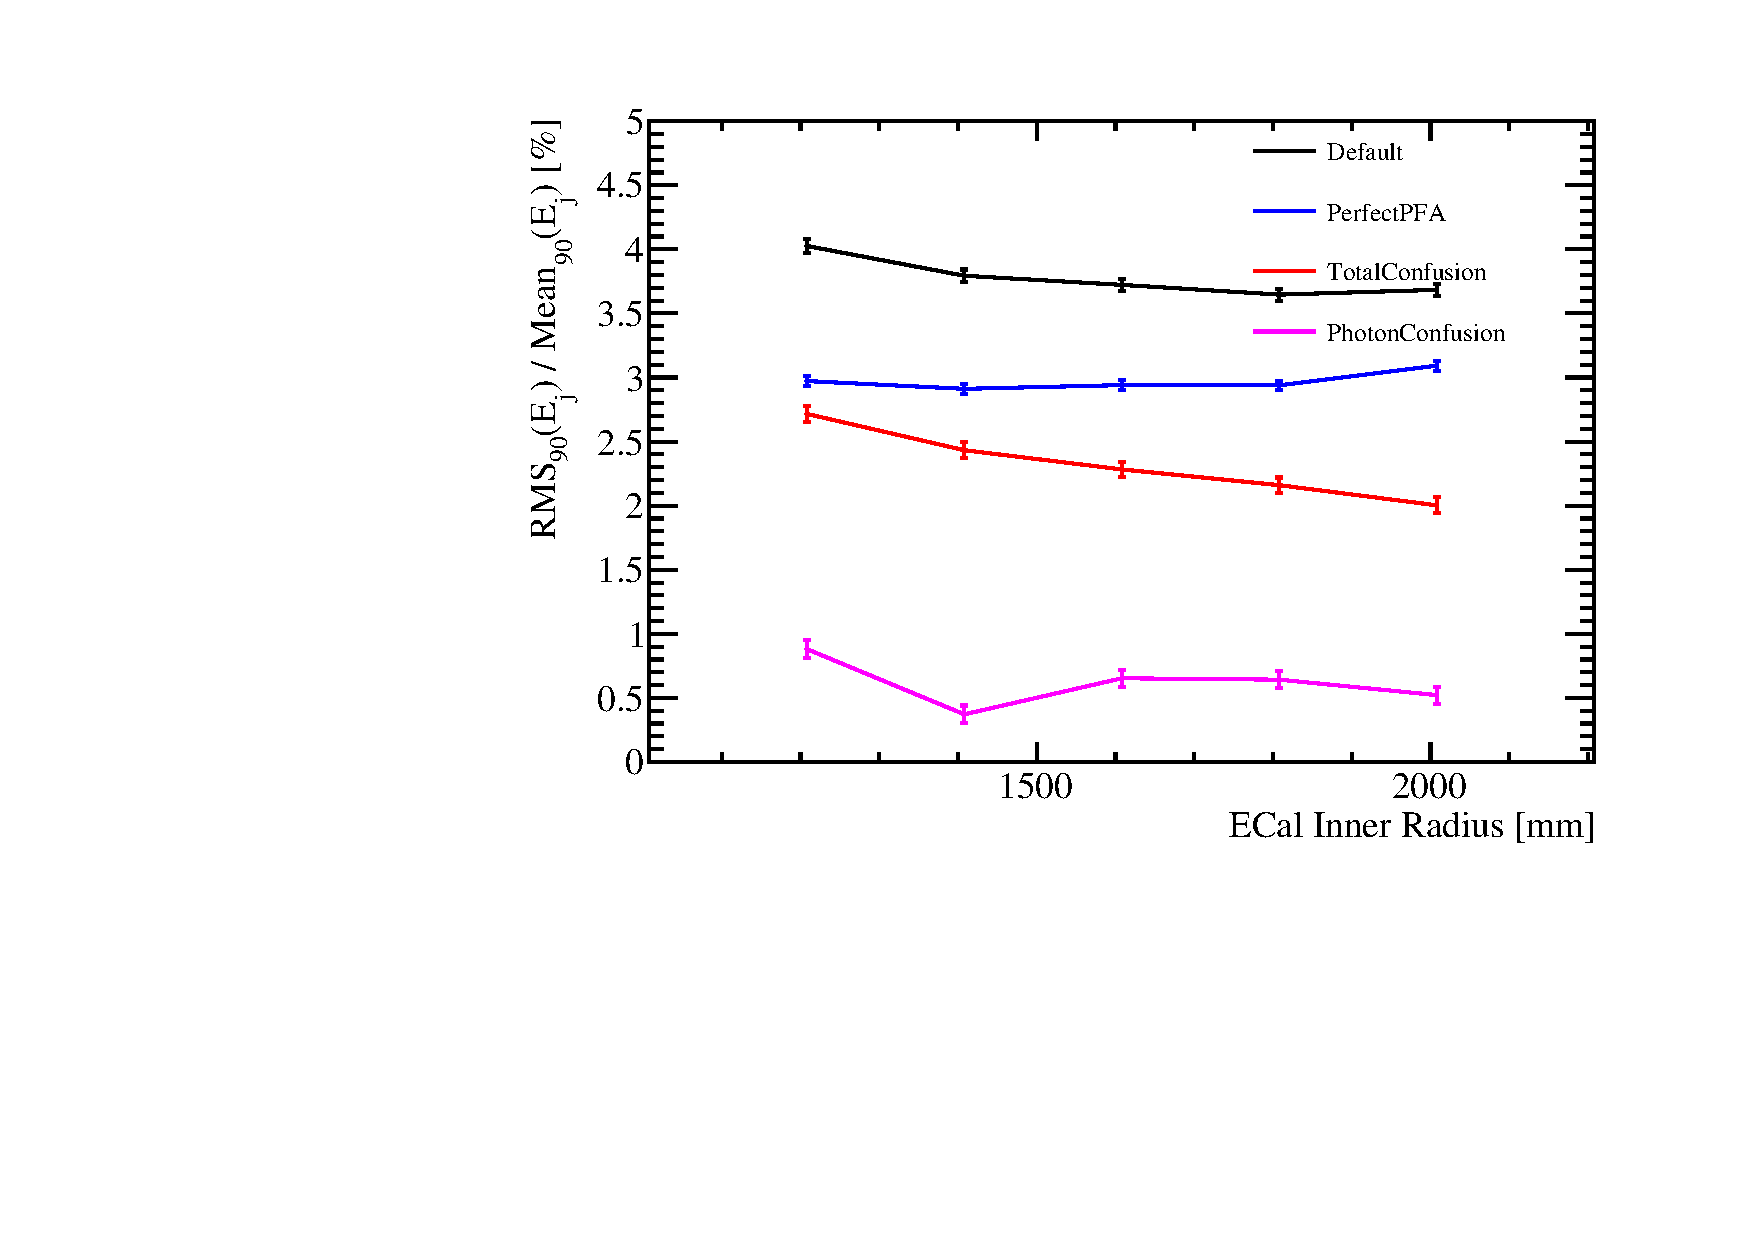
\includegraphics[width=0.5\textwidth]{OptimisationStudies/Plots/JetEnergyResolutions/JER_vs_ECalInnerRadius_91GeV_DiJet_Breakdown.pdf}}
\subfloat[]{\label{fig:ecalinnerr250break}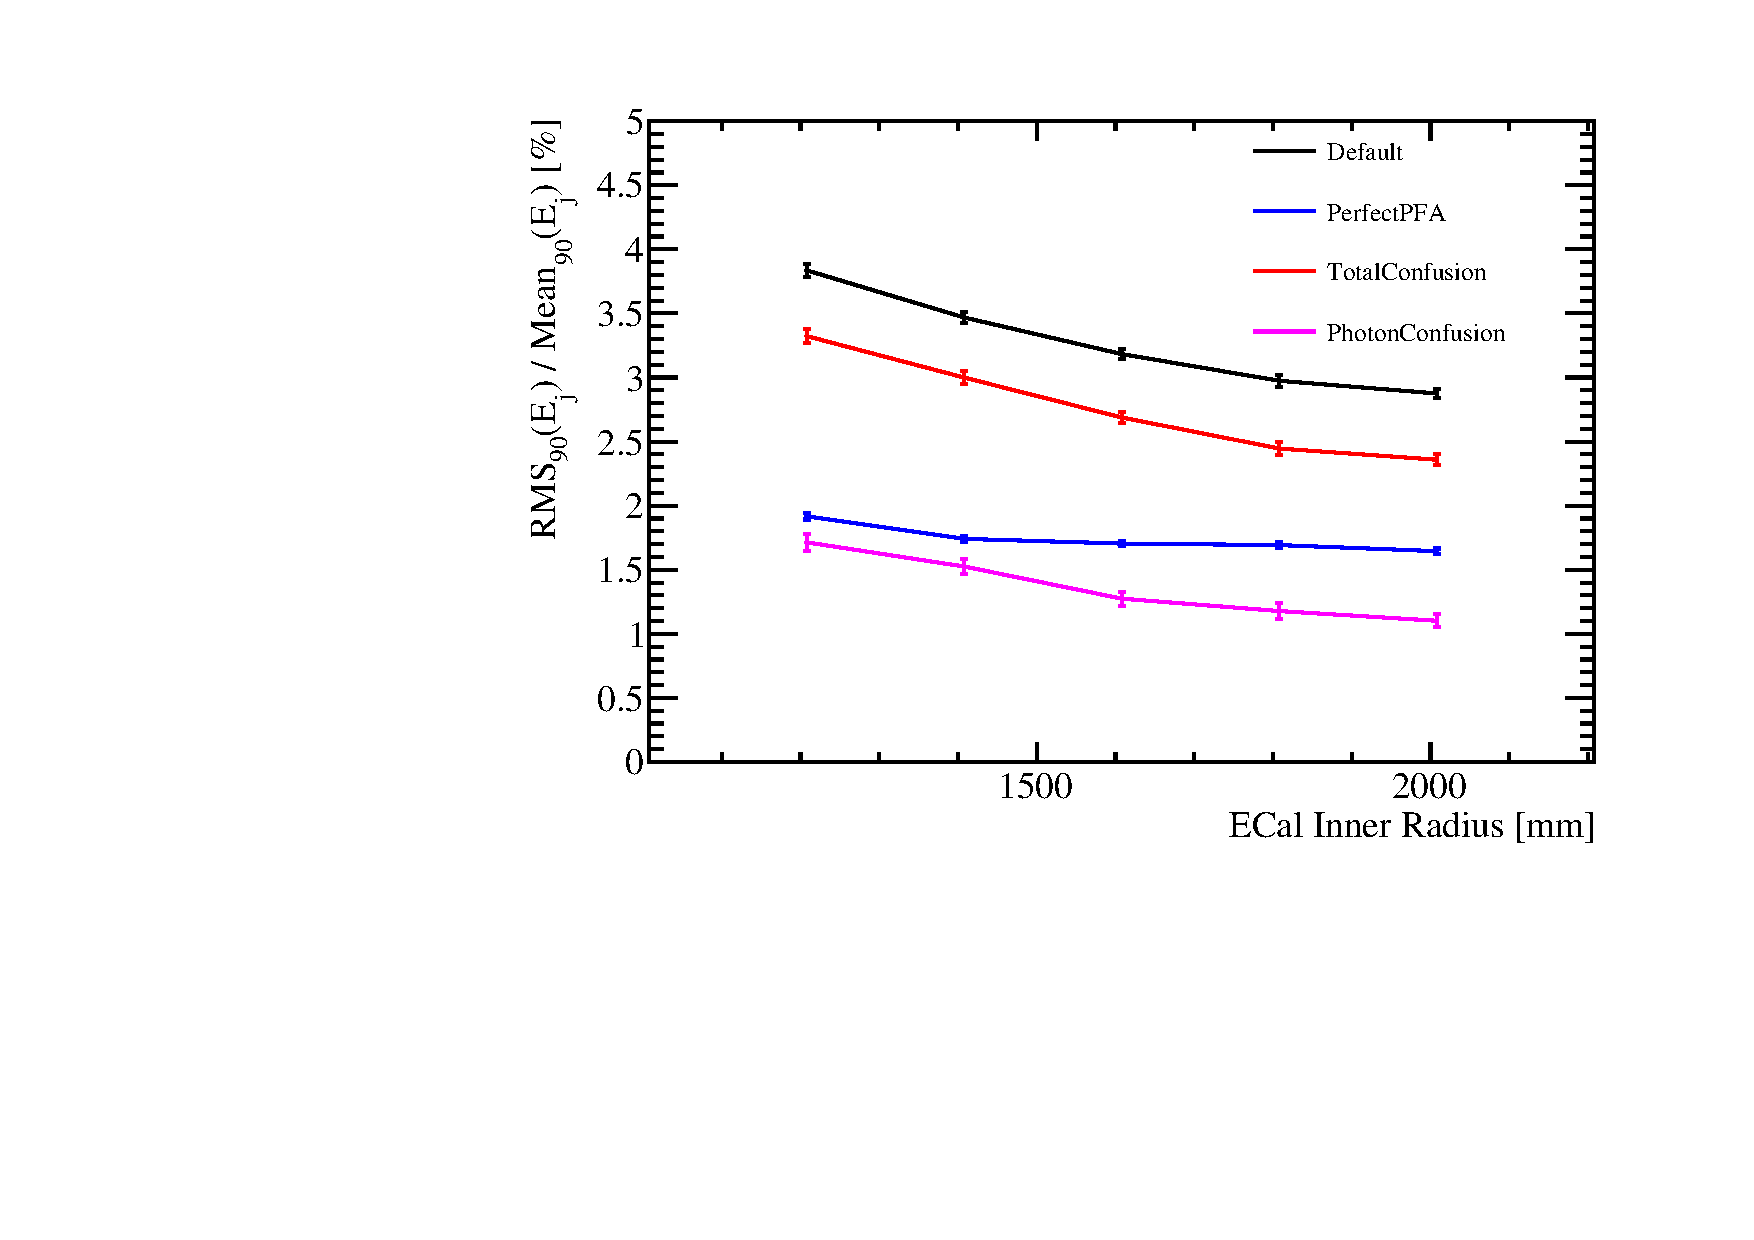
\includegraphics[width=0.5\textwidth]{OptimisationStudies/Plots/JetEnergyResolutions/JER_vs_ECalInnerRadius_500GeV_DiJet_Breakdown.pdf}}
\caption[Contributions to the jet energy resolution shown as function of the ECal inner radius using the nominal ILD detector model for \protect\subref{fig:ecalinnerr45break} 45~GeV jets and \protect\subref{fig:ecalinnerr250break} 250~GeV jets.  The black curves correspond to the standard reconstruction, the blue curves to the intrinsic energy resolution contribution to the jet energy resolution, the red curves to the confusion contribution to the jet energy resolution and the magenta curves to the confusion contribution to the jet energy resolution related solely to photon reconstruction.]{Contributions to the jet energy resolution shown as function of the ECal inner radius using the nominal ILD detector model for \protect\subref{fig:ecalinnerr45break} 45~GeV jets and \protect\subref{fig:ecalinnerr250break} 250~GeV jets.  The black curves correspond to the standard reconstruction, the blue curves to the intrinsic energy resolution contribution to the jet energy resolution, the red curves to the confusion contribution to the jet energy resolution and the magenta curves to the confusion contribution to the jet energy resolution related solely to photon reconstruction.}
\label{fig:ecalinnerrbreak}
\end{figure}

In conclusion, increasing the ECal inner radius benefits the jet energy resolution because it increases the separation between particles as they enter the calorimeter, which reduces confusion.

%========================================================================================
%========================================================================================

\section{Summary}
The effect of varying the configuration of the calorimeters, the magnetic field strength and the overall detector size on the single particle and jet energy resolutions were presented in this chapter.  For both the ECal and the HCal, the dominant factor determining the intrinsic energy resolution was the longitudinal sampling frequency.  However, the jet energy resolution had the strongest sensitivity to the ECal cell size, which shows that spatial recognition is more important when using particle flow calorimetry than intrinsic energy resolution.  The HCal cell size was found to be less significant than the ECal cell size for determining the jet energy resolution because separation of nearby particle showers in the HCal uses the spatial information gathered in the ECal.  In the particle flow paradigm, fine segmentation in the ECal can compensate for the coarser HCal granularities.  The jet energy resolution also showed a strong dependence on the magnetic field strength and the overall detector size.  Increasing both the magnetic field and overall detector size leads to greater separation of nearby particle showers in the calorimeters, which reduces the effect of confusion.  

%========================================================================================
%========================================================================================

